% Options for packages loaded elsewhere
% Options for packages loaded elsewhere
\PassOptionsToPackage{unicode}{hyperref}
\PassOptionsToPackage{hyphens}{url}
\PassOptionsToPackage{dvipsnames,svgnames,x11names}{xcolor}
%
\documentclass[
  letterpaper,
  DIV=11,
  numbers=noendperiod]{scrartcl}
\usepackage{xcolor}
\usepackage{amsmath,amssymb}
\setcounter{secnumdepth}{5}
\usepackage{iftex}
\ifPDFTeX
  \usepackage[T1]{fontenc}
  \usepackage[utf8]{inputenc}
  \usepackage{textcomp} % provide euro and other symbols
\else % if luatex or xetex
  \usepackage{unicode-math} % this also loads fontspec
  \defaultfontfeatures{Scale=MatchLowercase}
  \defaultfontfeatures[\rmfamily]{Ligatures=TeX,Scale=1}
\fi
\usepackage{lmodern}
\ifPDFTeX\else
  % xetex/luatex font selection
\fi
% Use upquote if available, for straight quotes in verbatim environments
\IfFileExists{upquote.sty}{\usepackage{upquote}}{}
\IfFileExists{microtype.sty}{% use microtype if available
  \usepackage[]{microtype}
  \UseMicrotypeSet[protrusion]{basicmath} % disable protrusion for tt fonts
}{}
\makeatletter
\@ifundefined{KOMAClassName}{% if non-KOMA class
  \IfFileExists{parskip.sty}{%
    \usepackage{parskip}
  }{% else
    \setlength{\parindent}{0pt}
    \setlength{\parskip}{6pt plus 2pt minus 1pt}}
}{% if KOMA class
  \KOMAoptions{parskip=half}}
\makeatother
% Make \paragraph and \subparagraph free-standing
\makeatletter
\ifx\paragraph\undefined\else
  \let\oldparagraph\paragraph
  \renewcommand{\paragraph}{
    \@ifstar
      \xxxParagraphStar
      \xxxParagraphNoStar
  }
  \newcommand{\xxxParagraphStar}[1]{\oldparagraph*{#1}\mbox{}}
  \newcommand{\xxxParagraphNoStar}[1]{\oldparagraph{#1}\mbox{}}
\fi
\ifx\subparagraph\undefined\else
  \let\oldsubparagraph\subparagraph
  \renewcommand{\subparagraph}{
    \@ifstar
      \xxxSubParagraphStar
      \xxxSubParagraphNoStar
  }
  \newcommand{\xxxSubParagraphStar}[1]{\oldsubparagraph*{#1}\mbox{}}
  \newcommand{\xxxSubParagraphNoStar}[1]{\oldsubparagraph{#1}\mbox{}}
\fi
\makeatother


\usepackage{longtable,booktabs,array}
\usepackage{calc} % for calculating minipage widths
% Correct order of tables after \paragraph or \subparagraph
\usepackage{etoolbox}
\makeatletter
\patchcmd\longtable{\par}{\if@noskipsec\mbox{}\fi\par}{}{}
\makeatother
% Allow footnotes in longtable head/foot
\IfFileExists{footnotehyper.sty}{\usepackage{footnotehyper}}{\usepackage{footnote}}
\makesavenoteenv{longtable}
\usepackage{graphicx}
\makeatletter
\newsavebox\pandoc@box
\newcommand*\pandocbounded[1]{% scales image to fit in text height/width
  \sbox\pandoc@box{#1}%
  \Gscale@div\@tempa{\textheight}{\dimexpr\ht\pandoc@box+\dp\pandoc@box\relax}%
  \Gscale@div\@tempb{\linewidth}{\wd\pandoc@box}%
  \ifdim\@tempb\p@<\@tempa\p@\let\@tempa\@tempb\fi% select the smaller of both
  \ifdim\@tempa\p@<\p@\scalebox{\@tempa}{\usebox\pandoc@box}%
  \else\usebox{\pandoc@box}%
  \fi%
}
% Set default figure placement to htbp
\def\fps@figure{htbp}
\makeatother





\setlength{\emergencystretch}{3em} % prevent overfull lines

\providecommand{\tightlist}{%
  \setlength{\itemsep}{0pt}\setlength{\parskip}{0pt}}



 


\KOMAoption{captions}{tableheading}
\makeatletter
\@ifpackageloaded{caption}{}{\usepackage{caption}}
\AtBeginDocument{%
\ifdefined\contentsname
  \renewcommand*\contentsname{Table of contents}
\else
  \newcommand\contentsname{Table of contents}
\fi
\ifdefined\listfigurename
  \renewcommand*\listfigurename{List of Figures}
\else
  \newcommand\listfigurename{List of Figures}
\fi
\ifdefined\listtablename
  \renewcommand*\listtablename{List of Tables}
\else
  \newcommand\listtablename{List of Tables}
\fi
\ifdefined\figurename
  \renewcommand*\figurename{Figure}
\else
  \newcommand\figurename{Figure}
\fi
\ifdefined\tablename
  \renewcommand*\tablename{Table}
\else
  \newcommand\tablename{Table}
\fi
}
\@ifpackageloaded{float}{}{\usepackage{float}}
\floatstyle{ruled}
\@ifundefined{c@chapter}{\newfloat{codelisting}{h}{lop}}{\newfloat{codelisting}{h}{lop}[chapter]}
\floatname{codelisting}{Listing}
\newcommand*\listoflistings{\listof{codelisting}{List of Listings}}
\makeatother
\makeatletter
\makeatother
\makeatletter
\@ifpackageloaded{caption}{}{\usepackage{caption}}
\@ifpackageloaded{subcaption}{}{\usepackage{subcaption}}
\makeatother
\usepackage{bookmark}
\IfFileExists{xurl.sty}{\usepackage{xurl}}{} % add URL line breaks if available
\urlstyle{same}
\hypersetup{
  pdftitle={Gut Microbiome Profiling in Pediatric Ulcerative Colitis},
  pdfauthor={Davide Maccarrone},
  colorlinks=true,
  linkcolor={blue},
  filecolor={Maroon},
  citecolor={Blue},
  urlcolor={Blue},
  pdfcreator={LaTeX via pandoc}}


\title{Gut Microbiome Profiling in Pediatric Ulcerative Colitis}
\usepackage{etoolbox}
\makeatletter
\providecommand{\subtitle}[1]{% add subtitle to \maketitle
  \apptocmd{\@title}{\par {\large #1 \par}}{}{}
}
\makeatother
\subtitle{16S rRNA amplicon analysis of PRJNA759642: from raw reads to
differential abundance}
\author{Davide Maccarrone}
\date{}
\begin{document}
\maketitle


\section{Executive summary}\label{executive-summary}

\textbf{Objective.} To characterize the gut microbiome of children with
ulcerative colitis (UC) compared with healthy children, using a
reproducible end-to-end 16S rRNA workflow on the public dataset
PRJNA759642.

\textbf{Dataset.} 42 fecal samples (19 UC, 23 healthy; age 7--21 years),
16S rRNA V4 amplicons, Illumina MiSeq 2 × 150 bp.

\textbf{Main findings.}

\begin{itemize}
\tightlist
\item
  \emph{Data quality and processing:} after DADA2 processing and chimera
  removal, the median number of non-chimeric reads per sample was
  \textbf{73,465}, and \textbf{73.4\%} of all input reads were retained
  overall.
\item
  \emph{Within-sample diversity:} Shannon diversity was \textbf{lower in
  UC} than in Healthy samples (median Shannon index: 2.44 vs 2.69;
  Wilcoxon p = \textbf{0.002}). After adjustment for age and gender,
  Shannon diversity in UC was \textbf{0.80-fold} that of Healthy samples
  (95\% CI: \textbf{0.71--0.90}). The group difference remained
  significant at every rarefaction depth tested (1,000--100,000 reads;
  Wilcoxon p = \textbf{0.002}) and after adjustment for library size.
\item
  \emph{Between-sample diversity:} disease status explained
  \textbf{9.7\%} of Bray-Curtis variation (PERMANOVA \emph{p} =
  \textbf{0.001}); dispersion did not differ significantly between
  groups (\emph{p} = \textbf{0.329}).
\item
  \emph{Differential abundance:} \textbf{28 taxonomic features} (22
  named families, one of them archaeal, and 6 unclassified lineages)
  differed between groups at BH-FDR \textless{} 0.25 (\textbf{12
  enriched} and \textbf{16 depleted} in UC), including
  \textbf{Enterobacteriaceae, Morganellaceae and Neisseriaceae}
  (enriched) and \textbf{Methanobacteriaceae and Barnesiellaceae}
  (depleted).
\end{itemize}

\textbf{Take-home message.} UC was associated with reduced within-sample
diversity and a distinct community composition compared with healthy
children, with a differential-abundance profile marked by an expansion
of Enterobacteriaceae-related taxa. Given the small cohort, the
exploratory significance threshold and the lack of adjustment for
treatment, these findings are associations to be validated in larger
cohorts.

\section{Background and objectives}\label{background-and-objectives}

Ulcerative colitis is a form of inflammatory bowel disease characterized
by inflammation and ulceration of the colon. Gut microbial dysbiosis has
been reported in both children and adults with UC. This report
reproduces and extends, with a fully scripted workflow, the 16S rRNA
analysis of the pediatric cohort published by Zuo et al.~(2022).

The analysis addresses four questions:

\begin{enumerate}
\def\labelenumi{\arabic{enumi}.}
\tightlist
\item
  Is the sequencing data of sufficient quality, and how many reads and
  variants are retained after processing?
\item
  How is the gut microbial community composed at the phylum level?
\item
  Do within-sample (alpha) and between-sample (beta) diversity differ
  between UC and healthy children, after accounting for age and gender?
\item
  Which microbial families differ in abundance between the two groups?
\end{enumerate}

\section{Dataset}\label{dataset}

\begin{longtable}[]{@{}
  >{\raggedright\arraybackslash}p{(\linewidth - 2\tabcolsep) * \real{0.3750}}
  >{\raggedright\arraybackslash}p{(\linewidth - 2\tabcolsep) * \real{0.6250}}@{}}
\caption{Characteristics of the analyzed
cohort.}\label{tbl-cohort}\tabularnewline
\toprule\noalign{}
\begin{minipage}[b]{\linewidth}\raggedright
Feature
\end{minipage} & \begin{minipage}[b]{\linewidth}\raggedright
Description
\end{minipage} \\
\midrule\noalign{}
\endfirsthead
\toprule\noalign{}
\begin{minipage}[b]{\linewidth}\raggedright
Feature
\end{minipage} & \begin{minipage}[b]{\linewidth}\raggedright
Description
\end{minipage} \\
\midrule\noalign{}
\endhead
\bottomrule\noalign{}
\endlastfoot
Source & NCBI SRA, BioProject PRJNA759642 (Zuo et al., 2022) \\
Sample type & Fecal samples, pediatric cohort \\
Samples analyzed & 42 (main cohort selected from the 114 runs of the
BioProject) \\
Groups & Healthy (n = 23), UC (n = 19) \\
Age & Healthy: median 14 (range 8--21) years; UC: median 15 (range
7--20) years \\
Gender & Healthy: 13 female / 10 male; UC: 9 female / 10 male \\
Sequencing & Illumina MiSeq, paired-end 2 × 150 bp, 16S rRNA V4 region
(515F/806R) \\
\end{longtable}

\section{Methods}\label{methods}

\subsection{Raw-read quality control}\label{raw-read-quality-control}

Raw reads were assessed with FastQC and summarized with MultiQC.
Aggregate quality profiles were additionally inspected in DADA2 to set
the truncation lengths. Primers had already been removed by the data
submitters before SRA deposition, and no adapter or primer contamination
was detected.

\subsection{ASV inference and
taxonomy}\label{asv-inference-and-taxonomy}

Reads were processed with DADA2: filtering and trimming (truncation at
140 bp for forward and 130 bp for reverse reads, maximum 2 expected
errors per read, no ambiguous bases, PhiX removal), separate error-rate
learning for forward and reverse reads, independent per-sample
denoising, paired-end merging, and removal of chimeras with the
consensus method. Taxonomy was assigned with the DADA2 naive Bayesian
classifier trained on SILVA 138.2 (non-redundant 99\% set), followed by
species-level assignment by exact matching.

\subsection{Community analysis}\label{community-analysis}

ASVs, taxonomy and metadata were integrated in a phyloseq object.
Analyses were performed at three taxonomic levels: phylum (composition),
genus (alpha and beta diversity) and family (differential abundance).
ASVs were aggregated with \texttt{tax\_glom} on the unfiltered table.
ASVs without an annotation at the chosen rank were retained as separate
``unclassified'' units, one for each distinct higher-rank lineage, and
are labelled with their lowest assigned rank.

\textbf{Alpha diversity.} The Shannon index was calculated on
genus-level counts and compared between groups with the Wilcoxon
rank-sum test. The effect of disease status was then estimated with a
linear model on log-transformed Shannon diversity, adjusted for age and
gender. Sequencing-depth effects were evaluated with Spearman
correlations (library size vs Shannon and vs observed genera), by adding
log10 library size to the model, and with a rarefaction sensitivity
analysis at 1,000, 5,000, 10,000, 30,000, 50,000 and 100,000 reads. At
each depth, the Shannon index was computed on each of 100 rarefied
tables and averaged per sample; samples with fewer reads than the target
depth were retained with all their reads.

\textbf{Beta diversity.} Bray-Curtis dissimilarities were computed on
genus-level relative abundances and visualized with PCoA. Group
differences were tested with PERMANOVA (\texttt{vegan::adonis2},
marginal effects of disease status, age and gender, 999 permutations)
and homogeneity of dispersion with \texttt{betadisper} and
\texttt{permutest} (999 permutations). Multiple Regression on distance
Matrices (\texttt{ecodist::MRM}, 999 permutations) was used to model
pairwise dissimilarities as a function of the disease-status combination
of each sample pair (Healthy--UC and UC--UC, with Healthy--Healthy as
reference), the gender combination (Female--Male and Female--Female,
with Male--Male as reference) and the age difference.

\textbf{Differential abundance.} Family-level counts were filtered
(families with zero counts in at least 90\% of samples, or with variance
below half of the median variance, were removed), normalized with TMM,
and tested for UC vs Healthy with the edgeR exact test after estimating
negative-binomial dispersions. P-values were adjusted with the
Benjamini--Hochberg procedure and taxa with FDR \textless{} 0.25 were
considered significant. This permissive threshold was adopted because of
the small sample size and the exploratory aim of the analysis; the taxa
that also passed FDR \textless{} 0.05 are reported separately.

All permutation procedures used a fixed seed (1234). The analysis was
run in R (v4.6.0); package versions are recorded in \texttt{renv.lock}
and in the session-information files saved by each script.

\section{Results}\label{results}

\subsection{Sequencing quality}\label{sequencing-quality}

Raw read counts per sample ranged from \textbf{22,274 to 1,592,901
(median 107,241)}. Base quality was generally high along the reads, with
localized fluctuations and a drop in the last cycles, and no adapter
contamination was observed (Figure~\ref{fig-qc-fw},
Figure~\ref{fig-qc-rv}). In the reverse reads, the proportion of reads
reaching each cycle (red line) begins to decline at about cycle 140.
Modules flagged as warnings or failures by FastQC (per-base sequence
content, duplication levels, overrepresented sequences, GC content) are
expected for amplicon data, in which all reads derive from the same
short, low-diversity locus, and do not indicate technical problems.

\begin{figure}[H]

\centering{

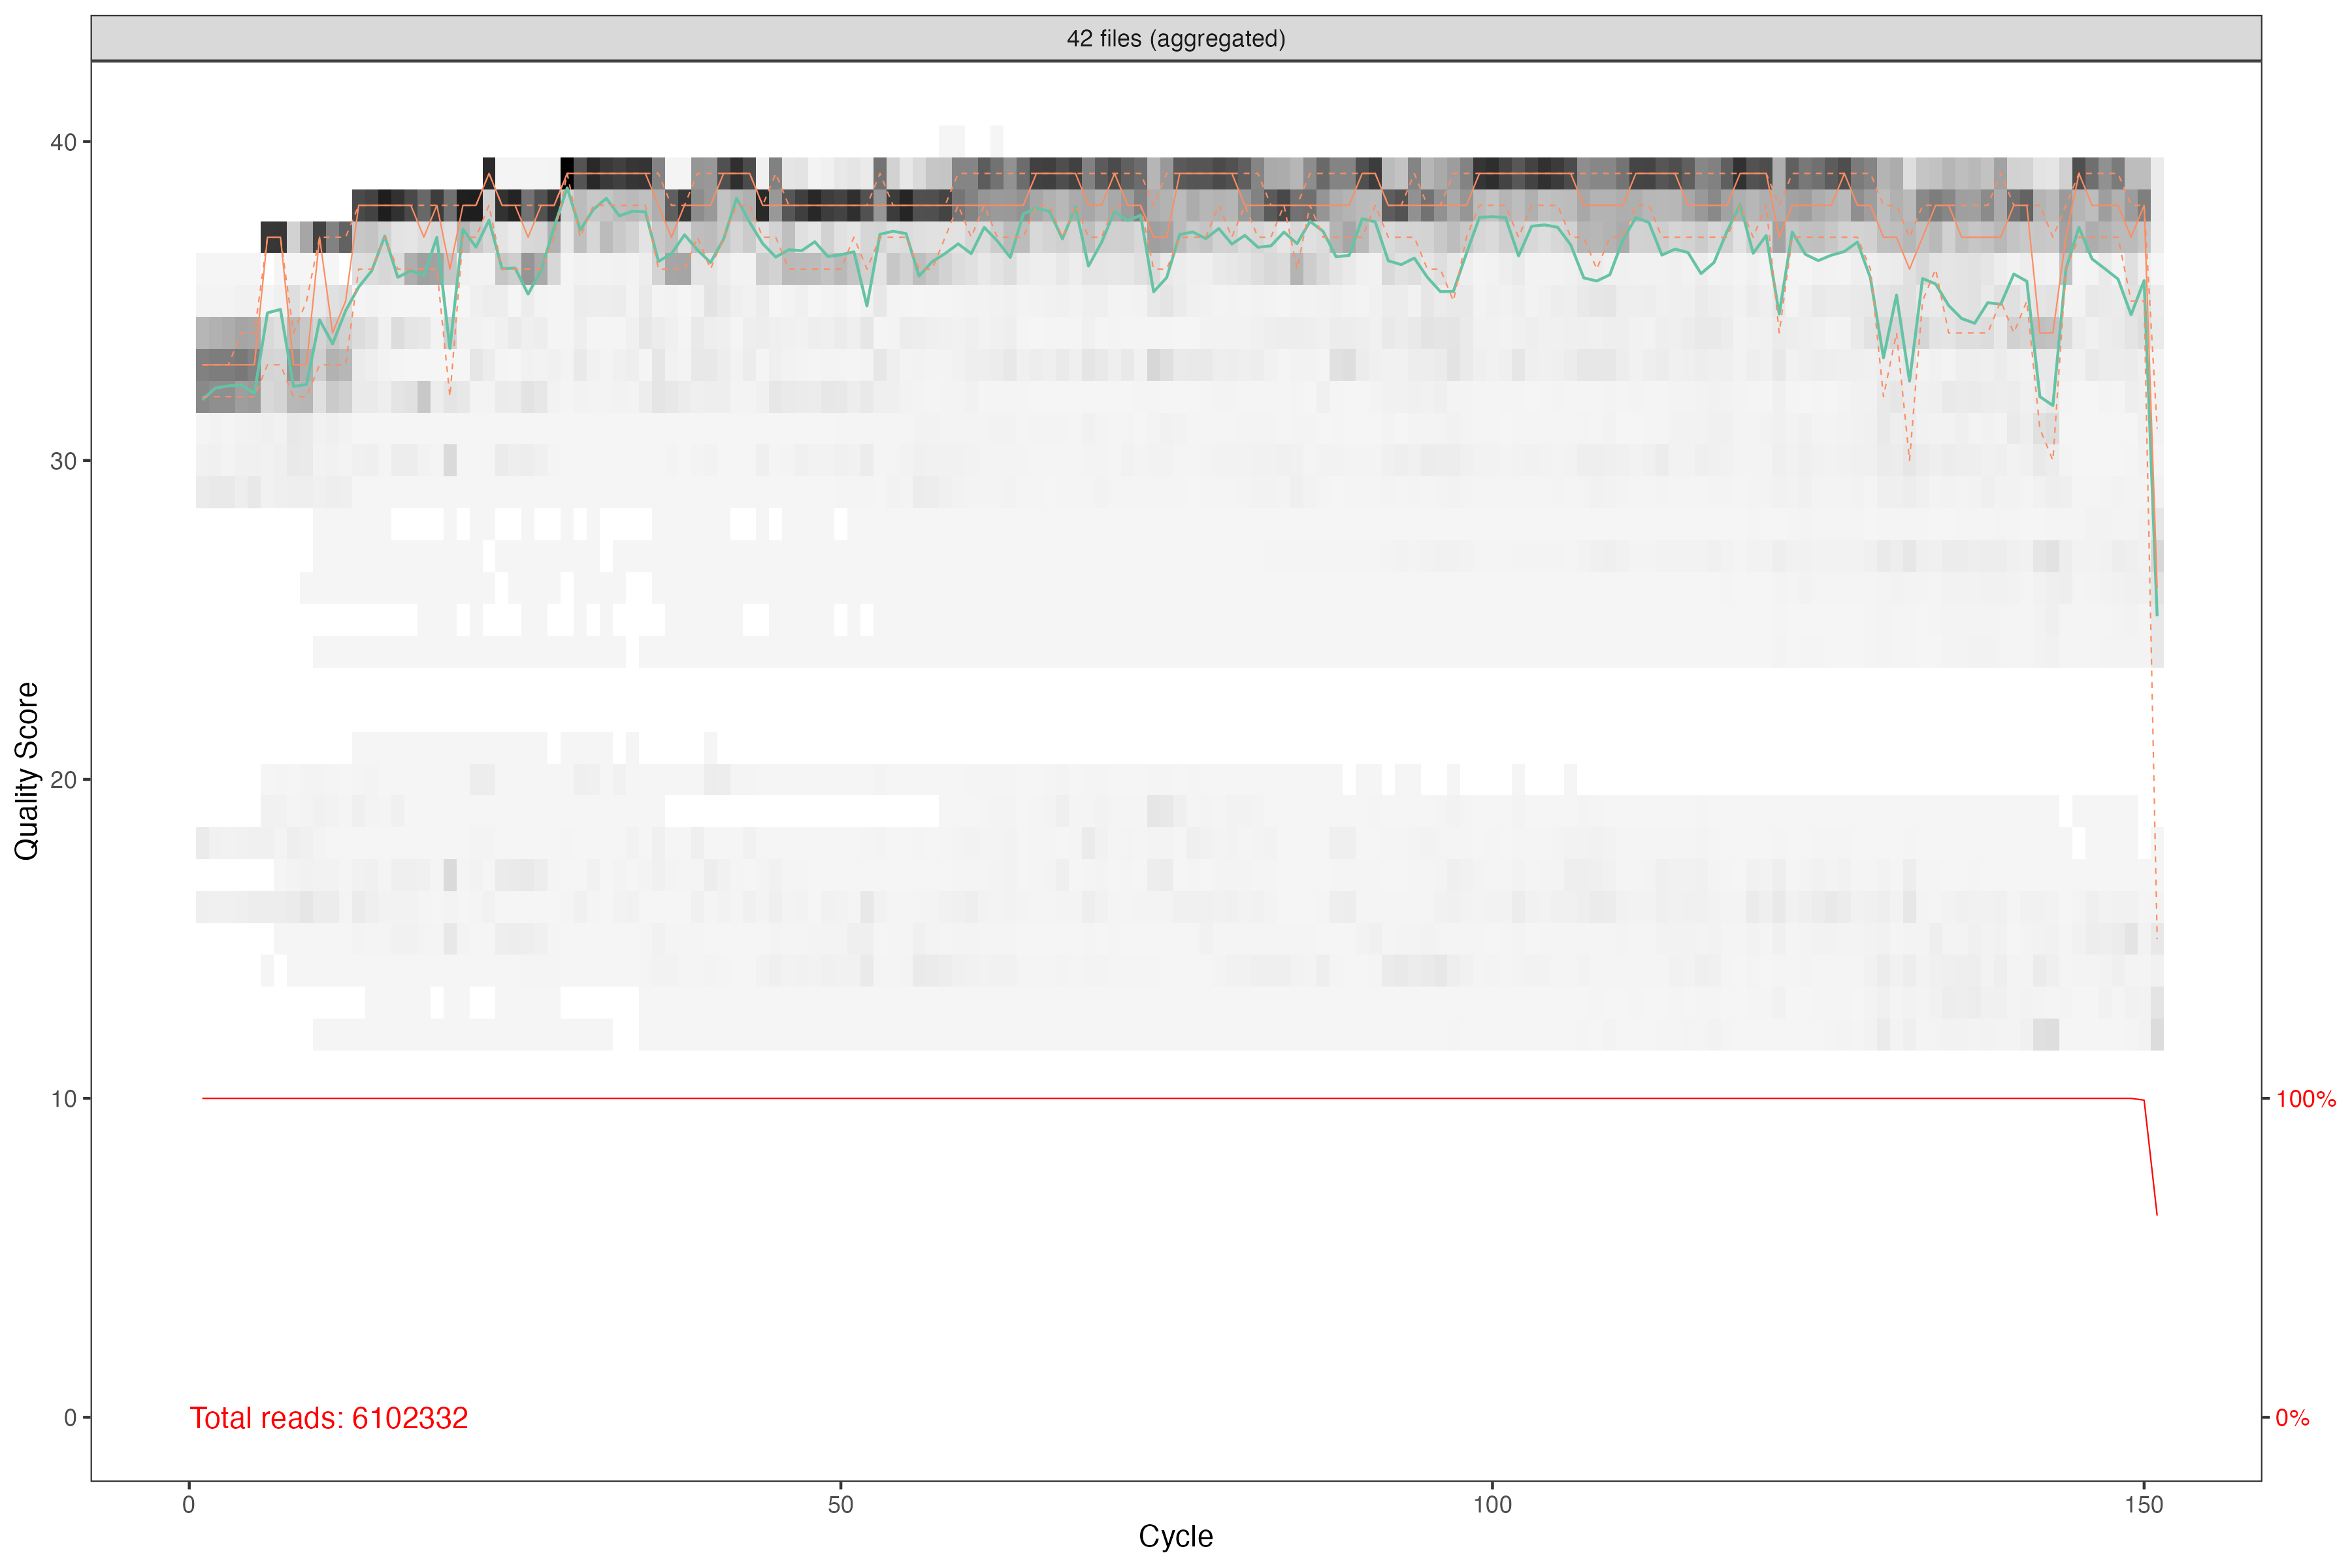
\includegraphics[width=0.85\linewidth,height=\textheight,keepaspectratio]{../results/plot/qc/QC_forward_aggregate.png}

}

\caption{\label{fig-qc-fw}Aggregate read-quality profile of the forward
reads (42 files).}

\end{figure}%

\begin{figure}[H]

\centering{

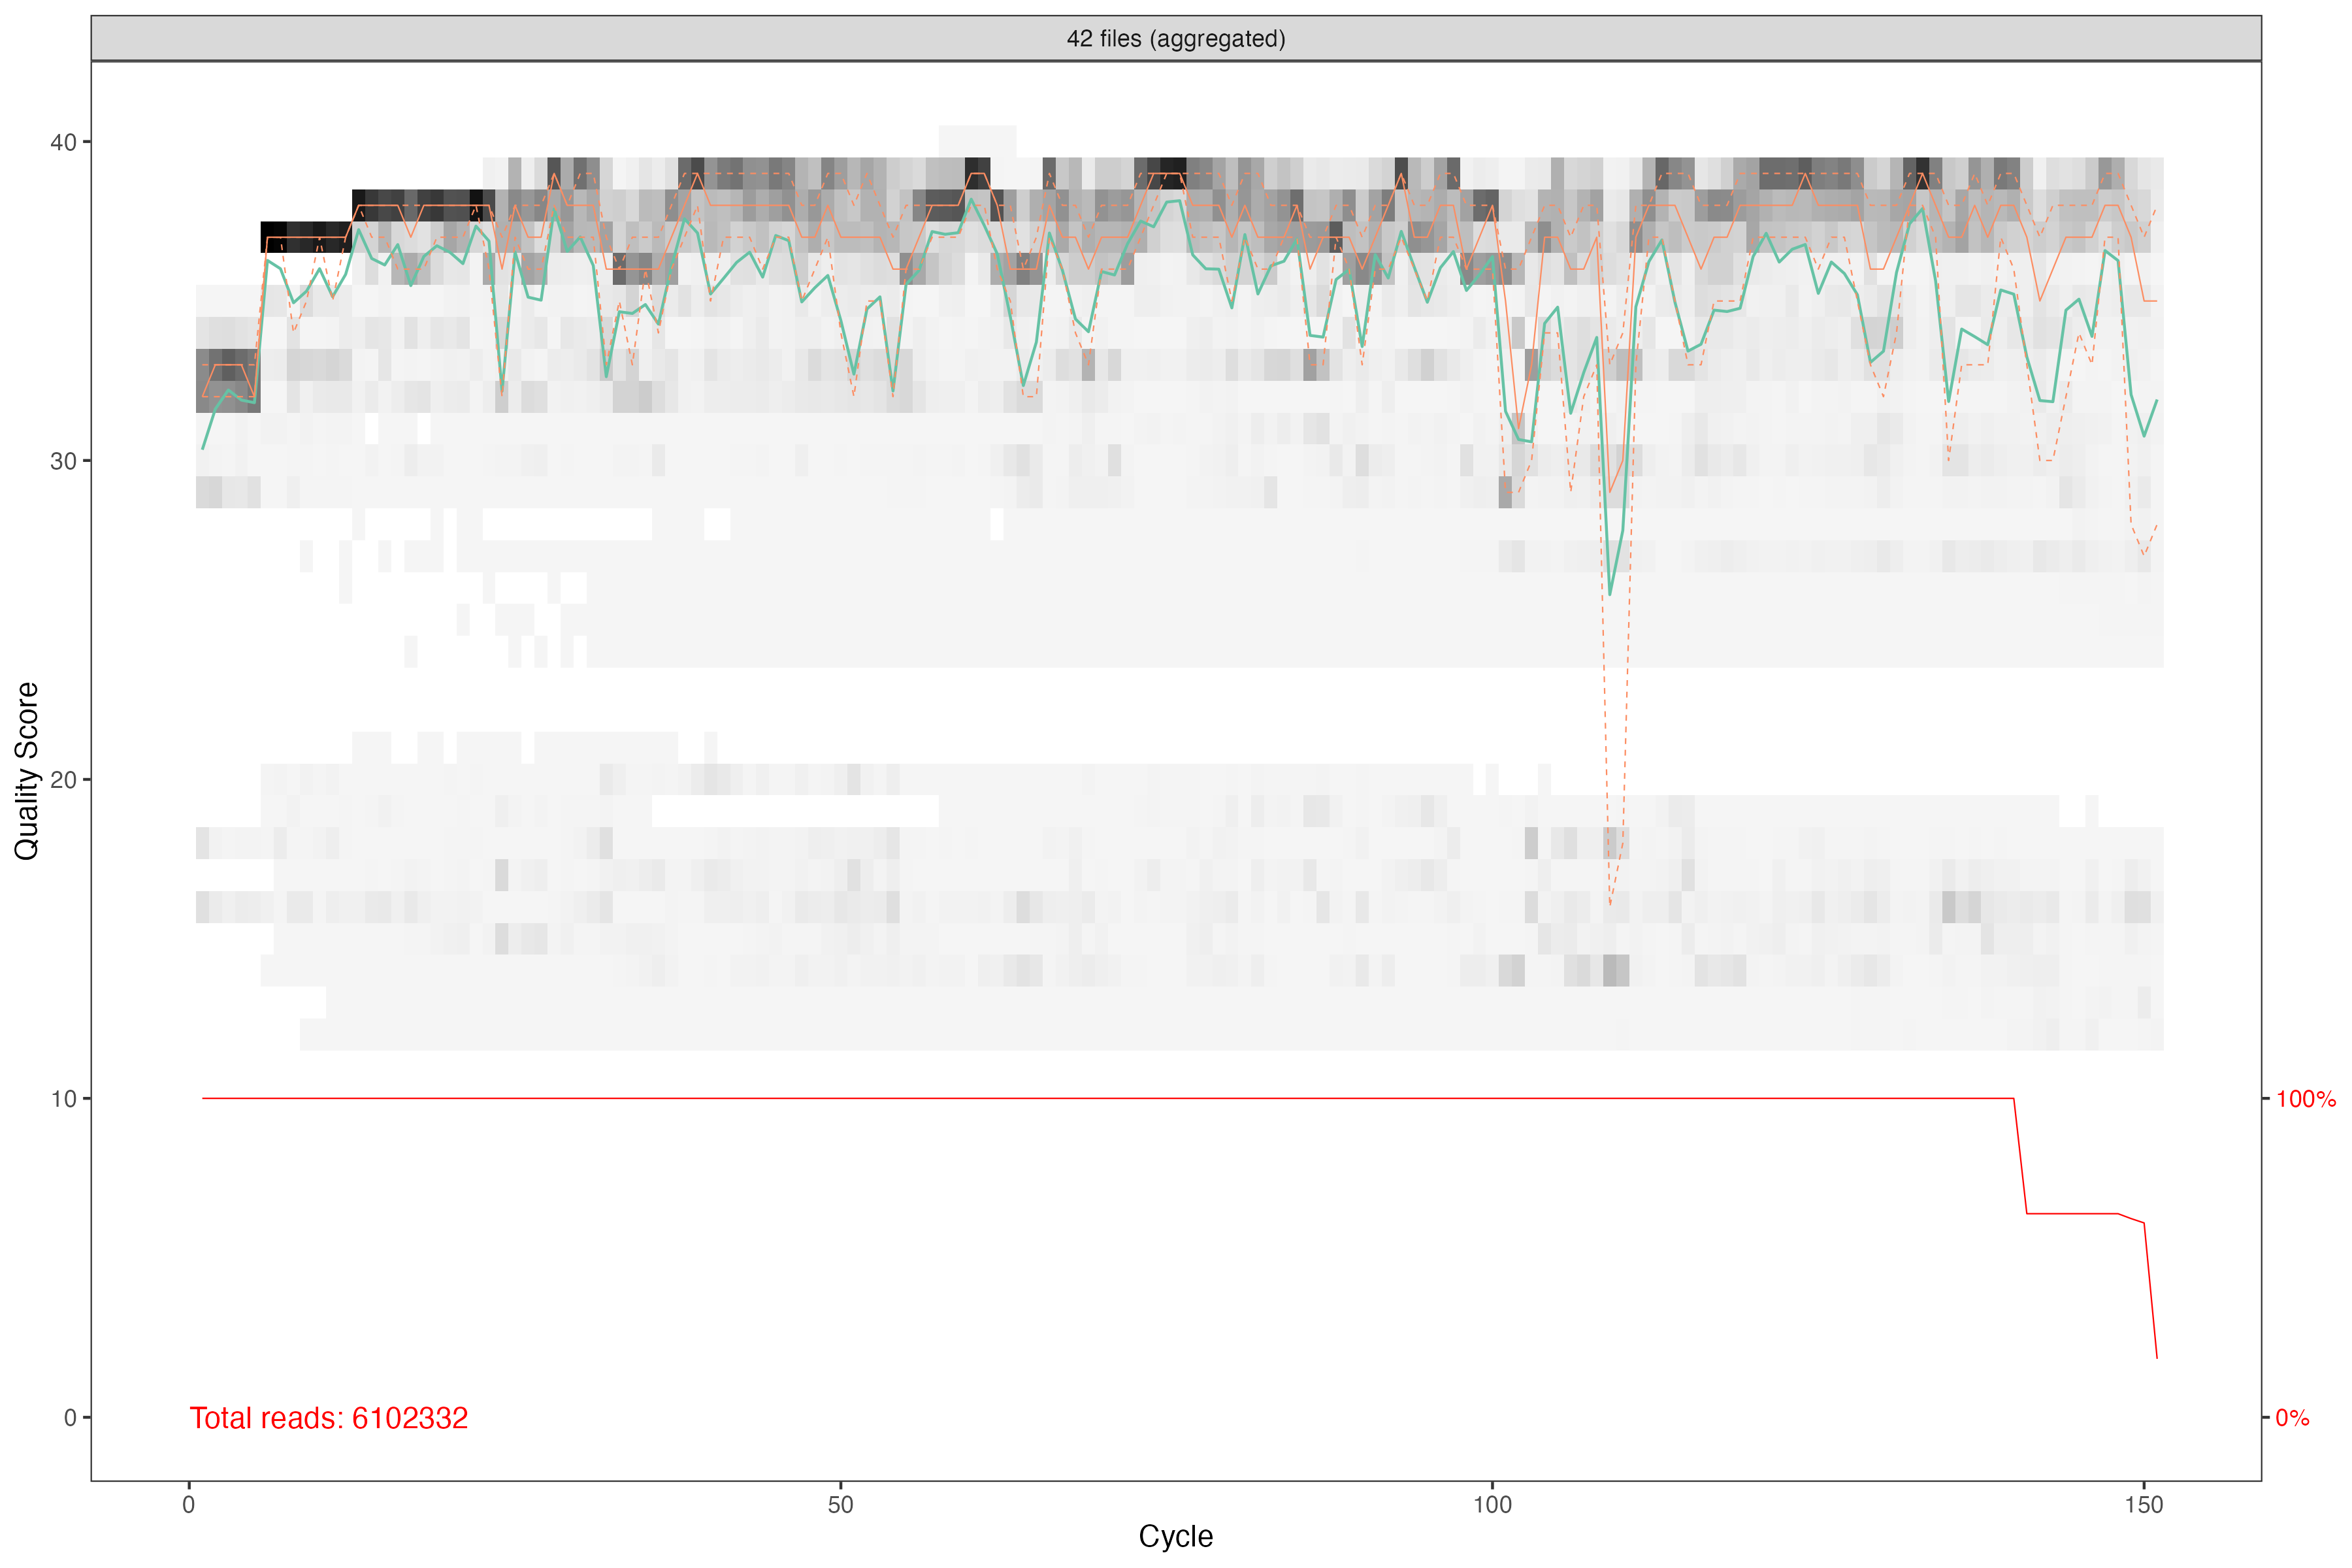
\includegraphics[width=0.85\linewidth,height=\textheight,keepaspectratio]{../results/plot/qc/QC_reverse_aggregate.png}

}

\caption{\label{fig-qc-rv}Aggregate read-quality profile of the reverse
reads (42 files).}

\end{figure}%

\subsection{ASV inference}\label{asv-inference}

Truncation lengths (140 bp forward, 130 bp reverse) were set on the
aggregate quality profiles to exclude the final cycles, where quality
drops and, in the reverse reads, part of the reads end, while leaving
enough overlap to merge the V4 amplicon. The learned error models
followed the observed error rates (Figure~\ref{fig-err-fw},
Figure~\ref{fig-err-rv}), and about 90\% of denoised reads were
successfully merged (89.7\%, ratio of medians; Table~\ref{tbl-track}).

\begin{figure}[H]

\centering{

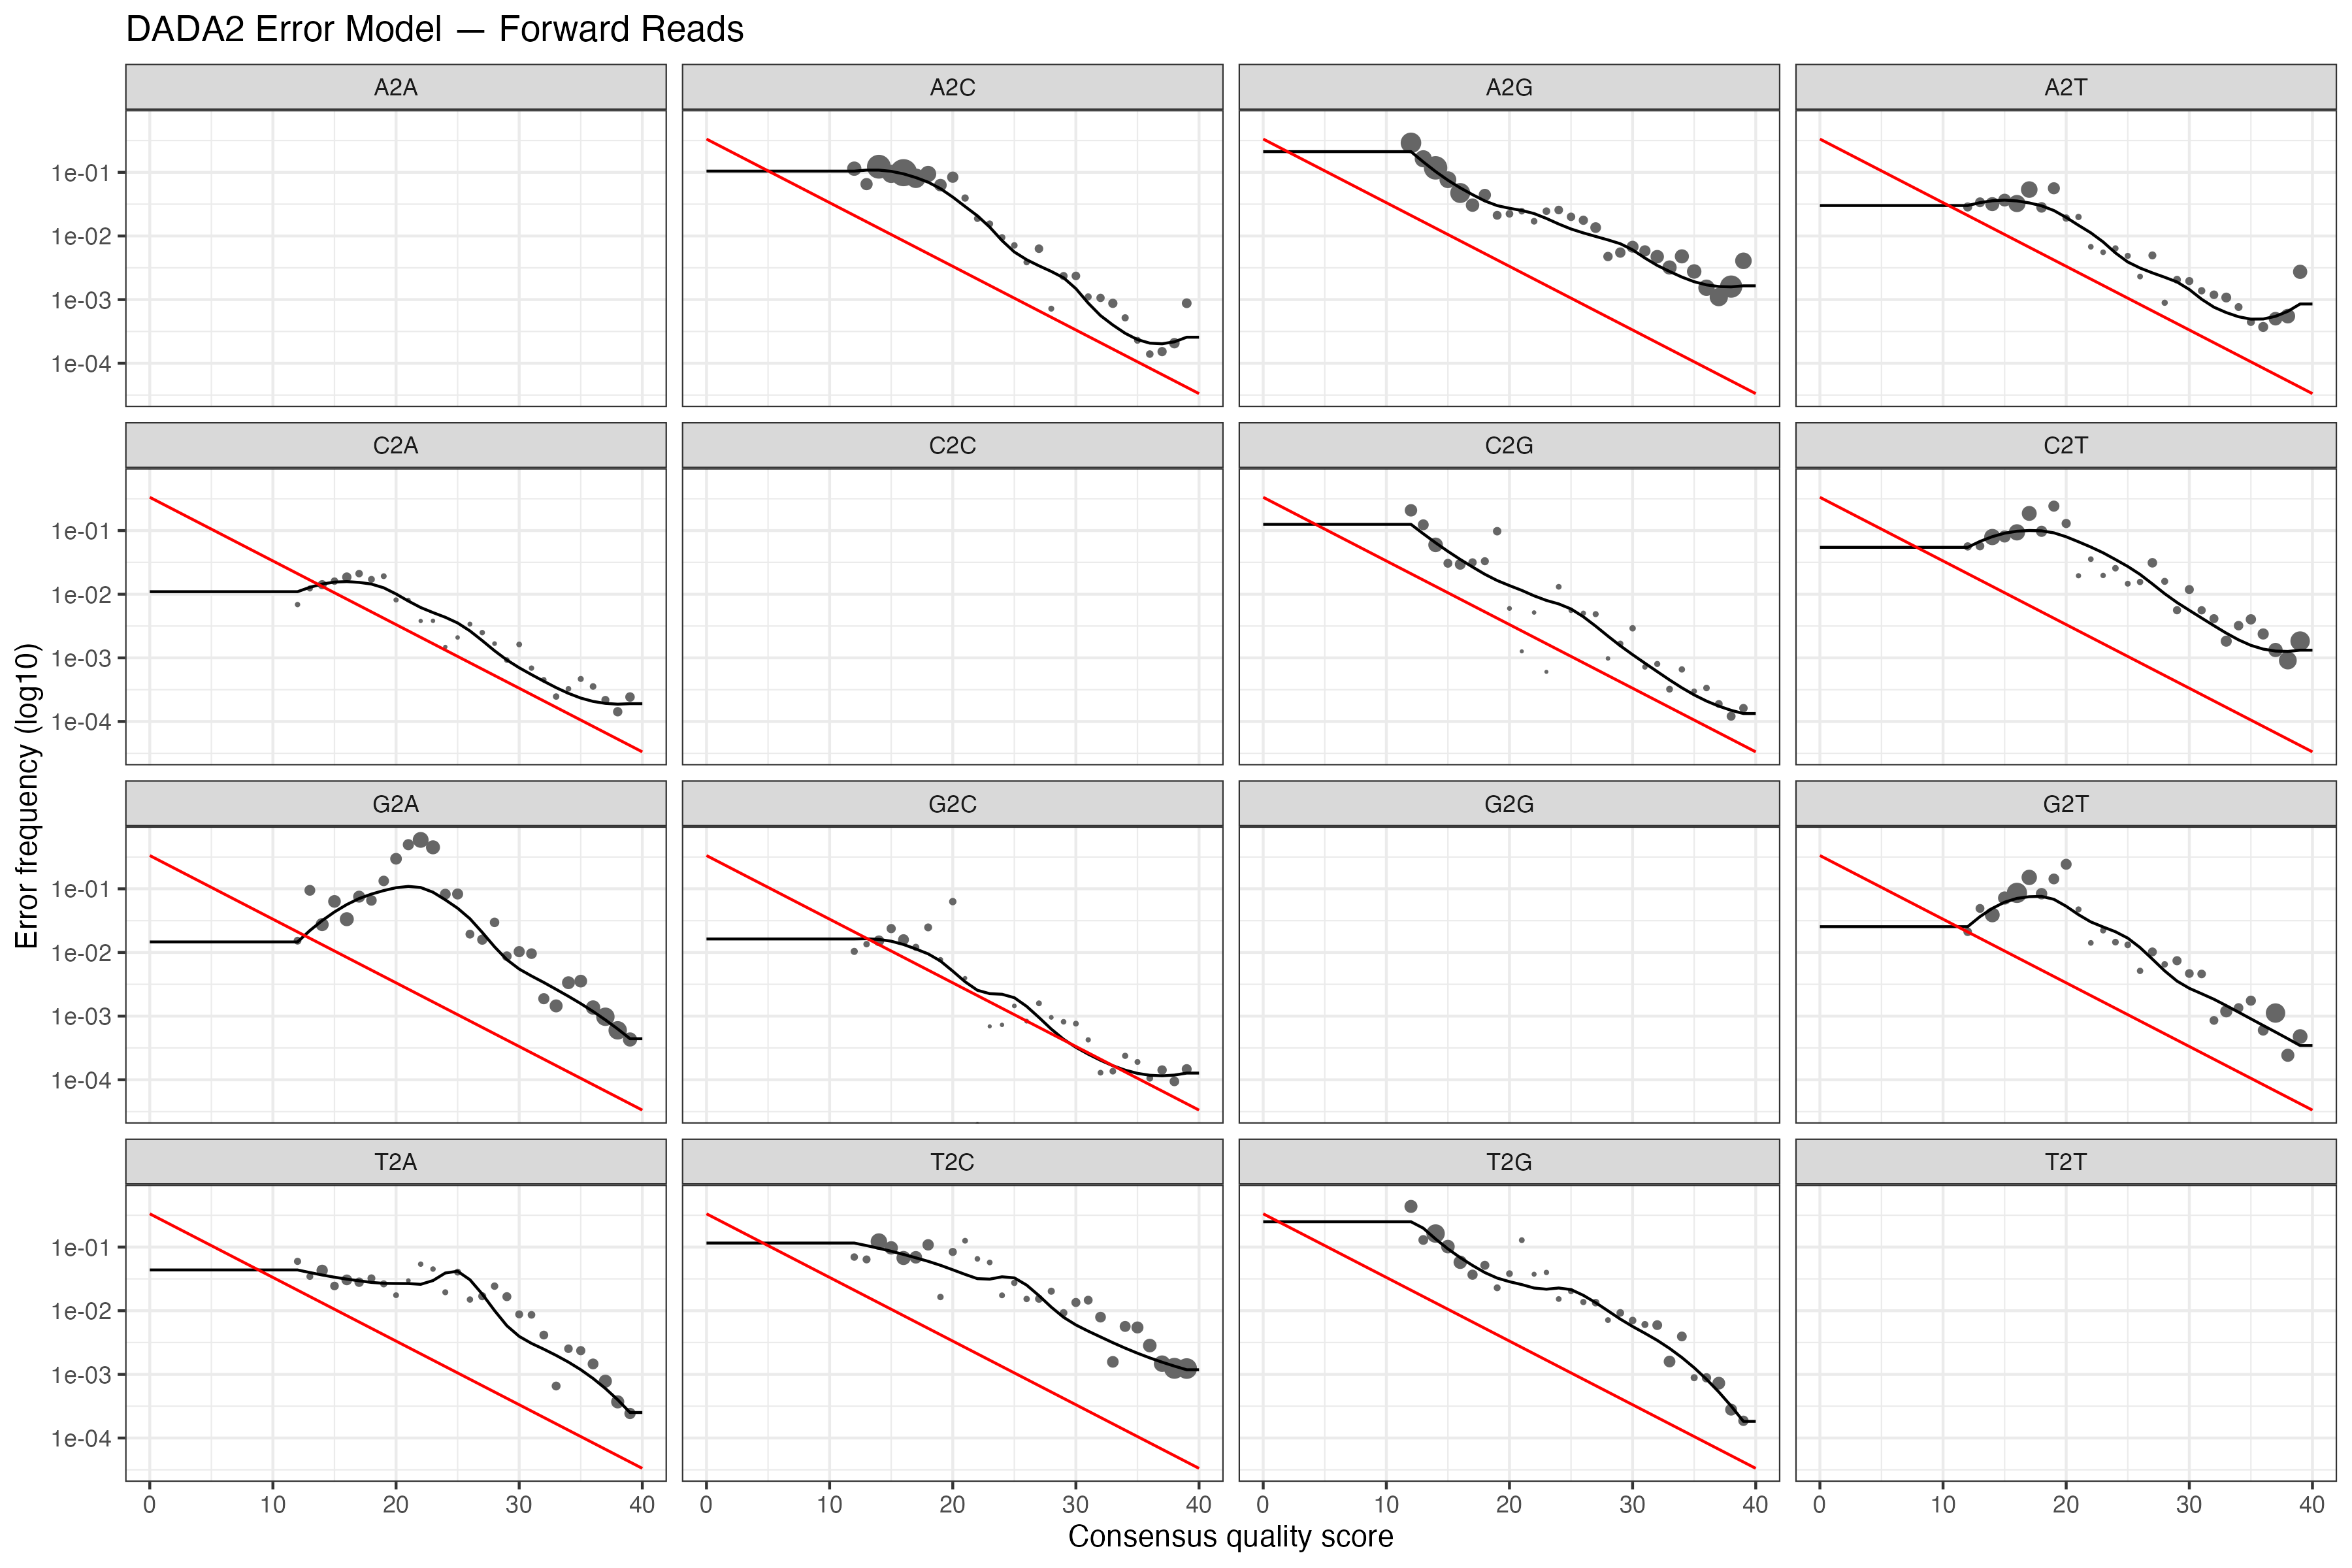
\includegraphics[width=1\linewidth,height=\textheight,keepaspectratio]{../results/plot/qc/dada2_error_model_forward.png}

}

\caption{\label{fig-err-fw}DADA2 error model for the forward reads.
Points are observed error rates, black lines the fitted model, red lines
the nominal Q-score expectation.}

\end{figure}%

\begin{figure}[H]

\centering{

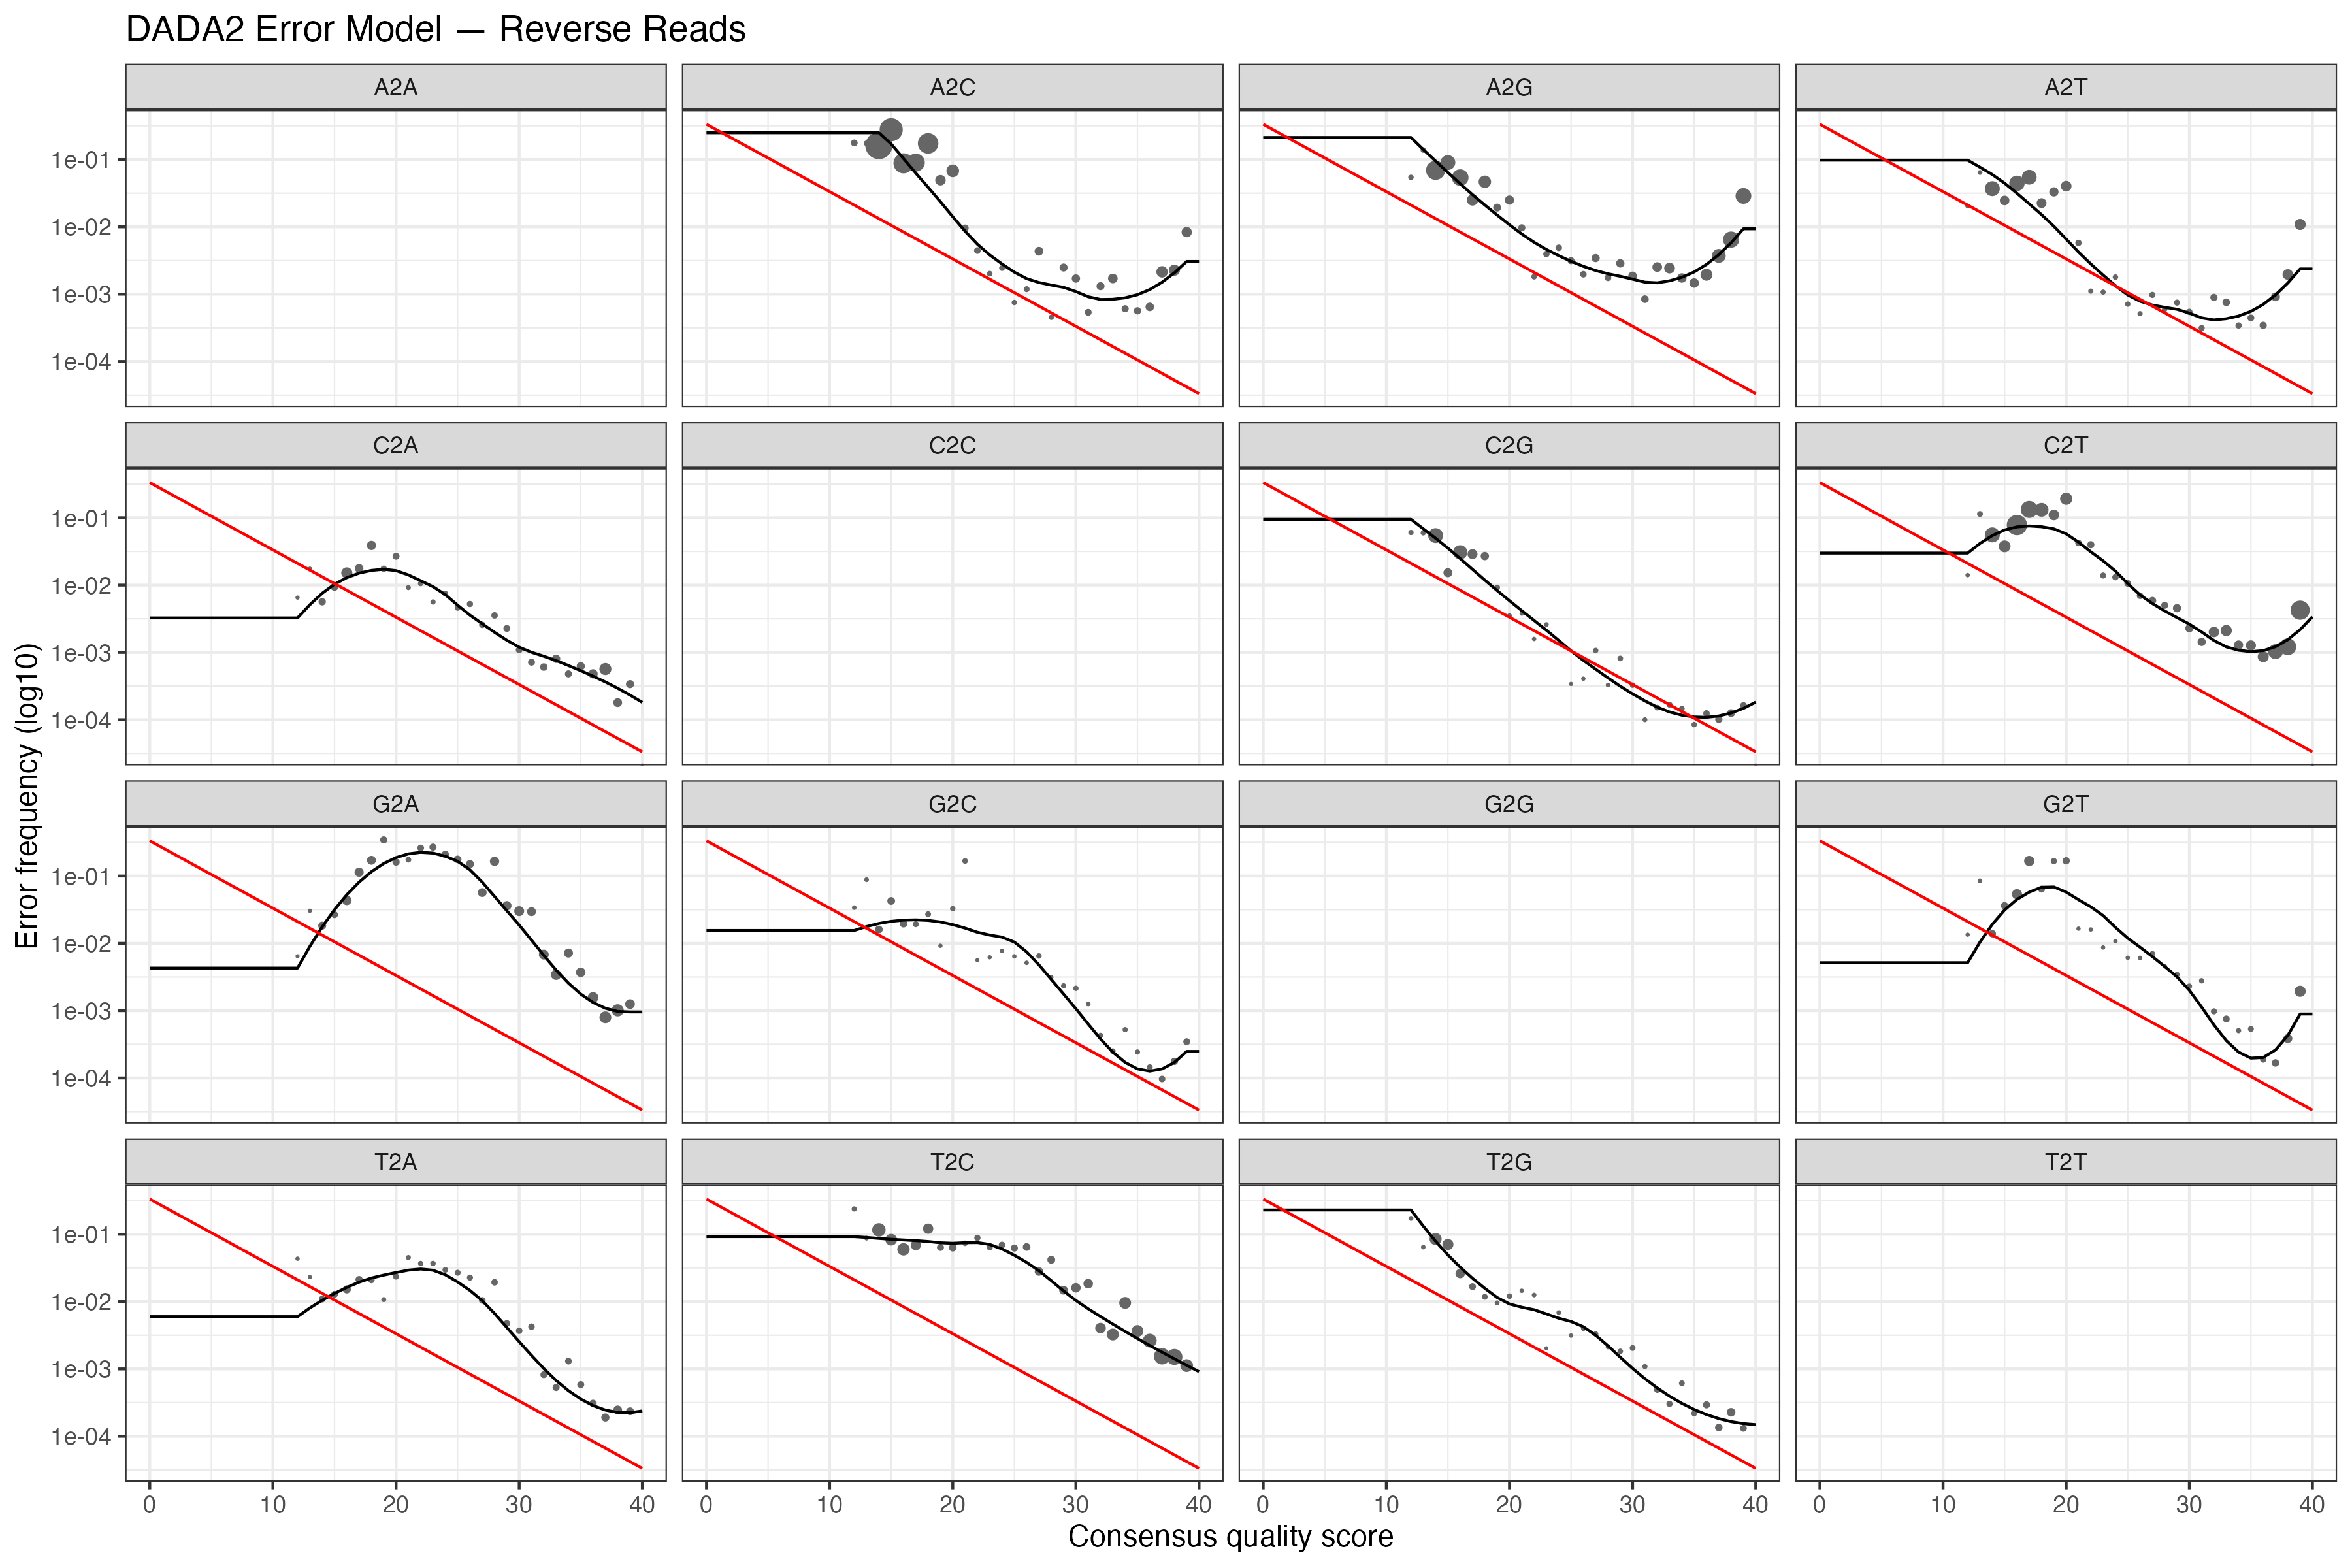
\includegraphics[width=1\linewidth,height=\textheight,keepaspectratio]{../results/plot/qc/dada2_error_model_reverse.png}

}

\caption{\label{fig-err-rv}DADA2 error model for the reverse reads.}

\end{figure}%

Table~\ref{tbl-track} summarizes how reads were retained along the
pipeline. In total, 3,564 non-chimeric ASVs were obtained across 42
samples; 20.57\% of merged reads were identified as chimeric and
removed, and overall 73.42\% of all input reads (summed across samples)
were retained.

\begin{longtable}[]{@{}
  >{\raggedright\arraybackslash}p{(\linewidth - 4\tabcolsep) * \real{0.3472}}
  >{\raggedright\arraybackslash}p{(\linewidth - 4\tabcolsep) * \real{0.3889}}
  >{\raggedleft\arraybackslash}p{(\linewidth - 4\tabcolsep) * \real{0.2639}}@{}}
\caption{Read tracking through the DADA2 pipeline. The last column is
the median of each step divided by the median input, and therefore
differs from the overall retention computed on summed reads
(73.42\%).}\label{tbl-track}\tabularnewline
\toprule\noalign{}
\begin{minipage}[b]{\linewidth}\raggedright
Step
\end{minipage} & \begin{minipage}[b]{\linewidth}\raggedright
Median reads per sample (range)
\end{minipage} & \begin{minipage}[b]{\linewidth}\raggedleft
Median reads, \% of median input
\end{minipage} \\
\midrule\noalign{}
\endfirsthead
\toprule\noalign{}
\begin{minipage}[b]{\linewidth}\raggedright
Step
\end{minipage} & \begin{minipage}[b]{\linewidth}\raggedright
Median reads per sample (range)
\end{minipage} & \begin{minipage}[b]{\linewidth}\raggedleft
Median reads, \% of median input
\end{minipage} \\
\midrule\noalign{}
\endhead
\bottomrule\noalign{}
\endlastfoot
Input & 107,241 (22,274--1,592,901) & 100 \\
Filtered & 106,790 (22,274--1,577,430) & 99.58 \\
Denoised (forward / reverse) & 105,622 / 105,414 (22,009--1,570,370 /
22,061--1,568,585) & 98.49 / 98.30 \\
Merged & 94,729 (20,363--1,503,715) & 88.33 \\
Non-chimeric & 73,465 (13,639--1,216,057) & 68.50 \\
\end{longtable}

\subsection{Taxonomic assignment and
composition}\label{taxonomic-assignment-and-composition}

Of the 3,564 ASVs, 99.4\% were classified at phylum level, 90.6\% at
family level, 67.8\% at genus level and 7.2\% at species level.

Sequencing depth after processing ranged from 13,639 to 1,216,057 reads
per sample (mean 106,668; Figure~\ref{fig-depth}). ASV prevalence was
low for most variants (median prevalence: 1 sample out of 42;
Figure~\ref{fig-prevalence}), as is typical of sparse microbiome tables.

\begin{figure}[H]

\centering{

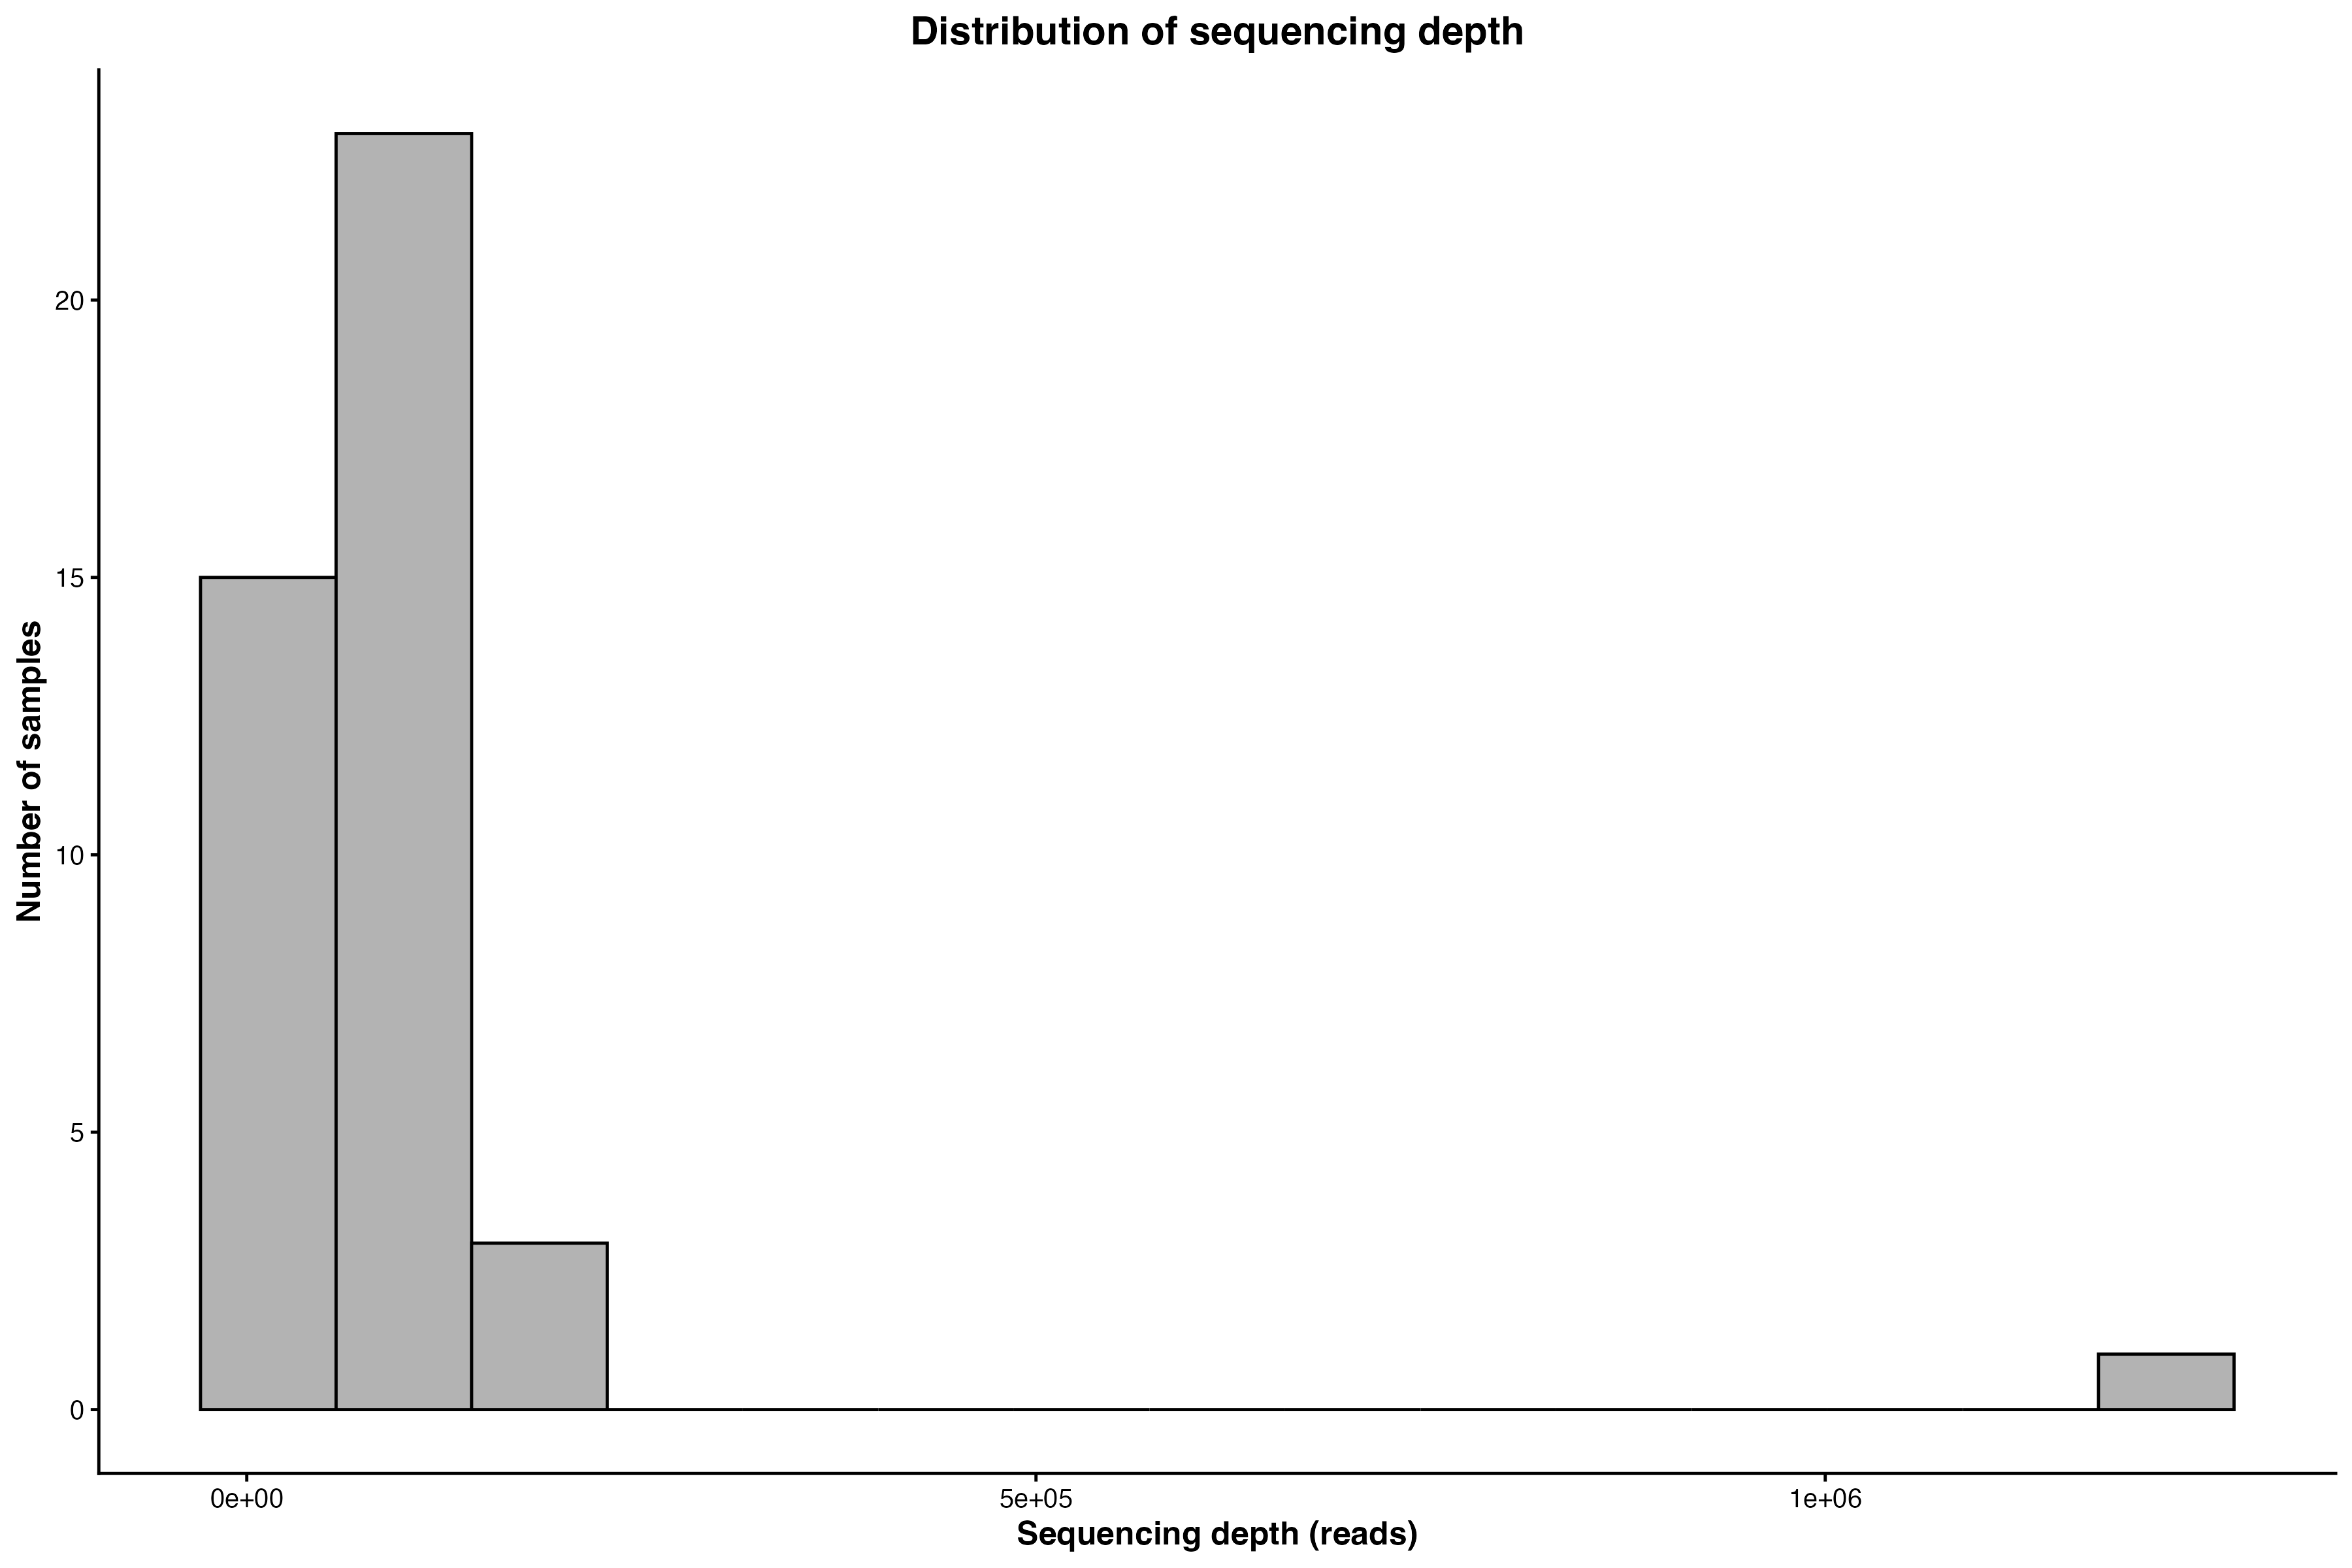
\includegraphics[width=1\linewidth,height=\textheight,keepaspectratio]{../results/plot/phyloseq_beta_alpha/sequencing_depth_distribution.png}

}

\caption{\label{fig-depth}Distribution of sequencing depth (reads per
sample after processing).}

\end{figure}%

\begin{figure}[H]

\centering{

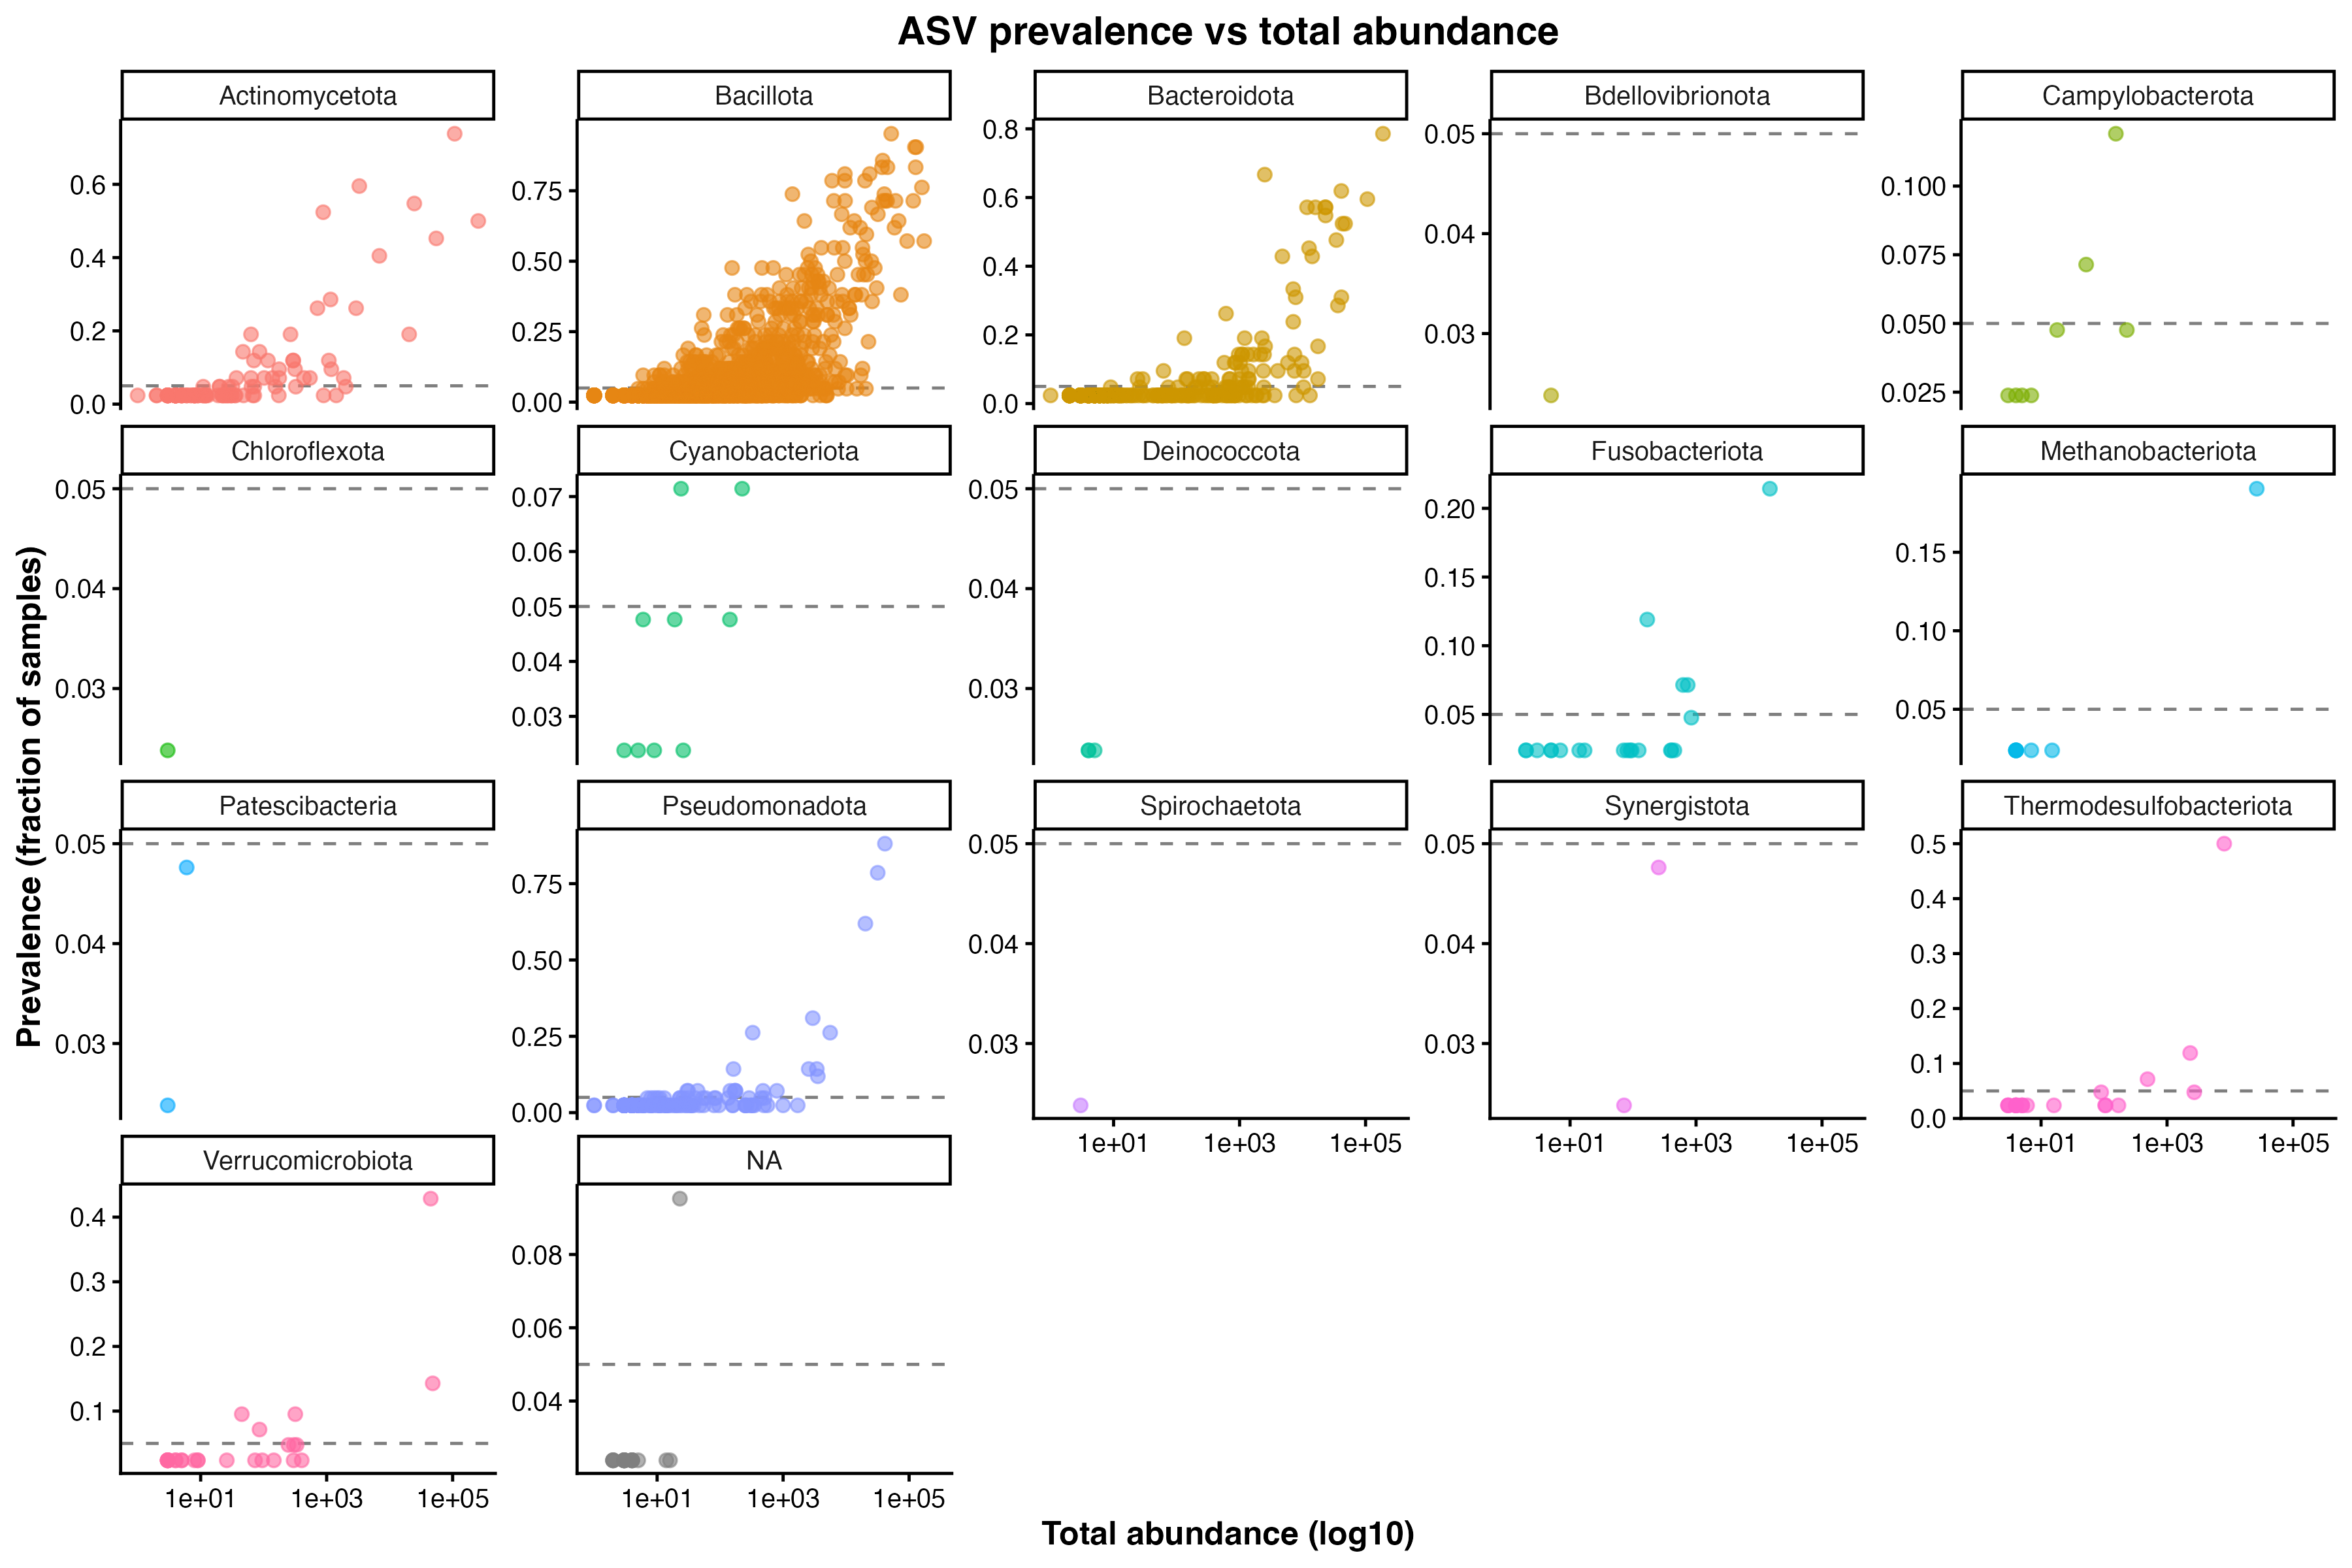
\includegraphics[width=1\linewidth,height=\textheight,keepaspectratio]{../results/plot/phyloseq_beta_alpha/asv_prevalence_vs_abundance.png}

}

\caption{\label{fig-prevalence}ASV prevalence versus total abundance, by
phylum. The dashed line marks 5\% of samples.}

\end{figure}%

At phylum level the community was dominated by four phyla with mean
relative abundance ≥ 2\% (Figure~\ref{fig-phylum},
Table~\ref{tbl-phyla}). Compared with Healthy samples, UC samples showed
a lower proportion of Bacillota (52.2\% vs 65.5\%) and Actinomycetota
(5.06\% vs 9.21\%), together with a higher proportion of Bacteroidota
(30.2\% vs 20.2\%) and Pseudomonadota (9.49\% vs 1.21\%). These are
descriptive means; group differences were tested at family level (see
Differential abundance).

\begin{figure}[H]

\centering{

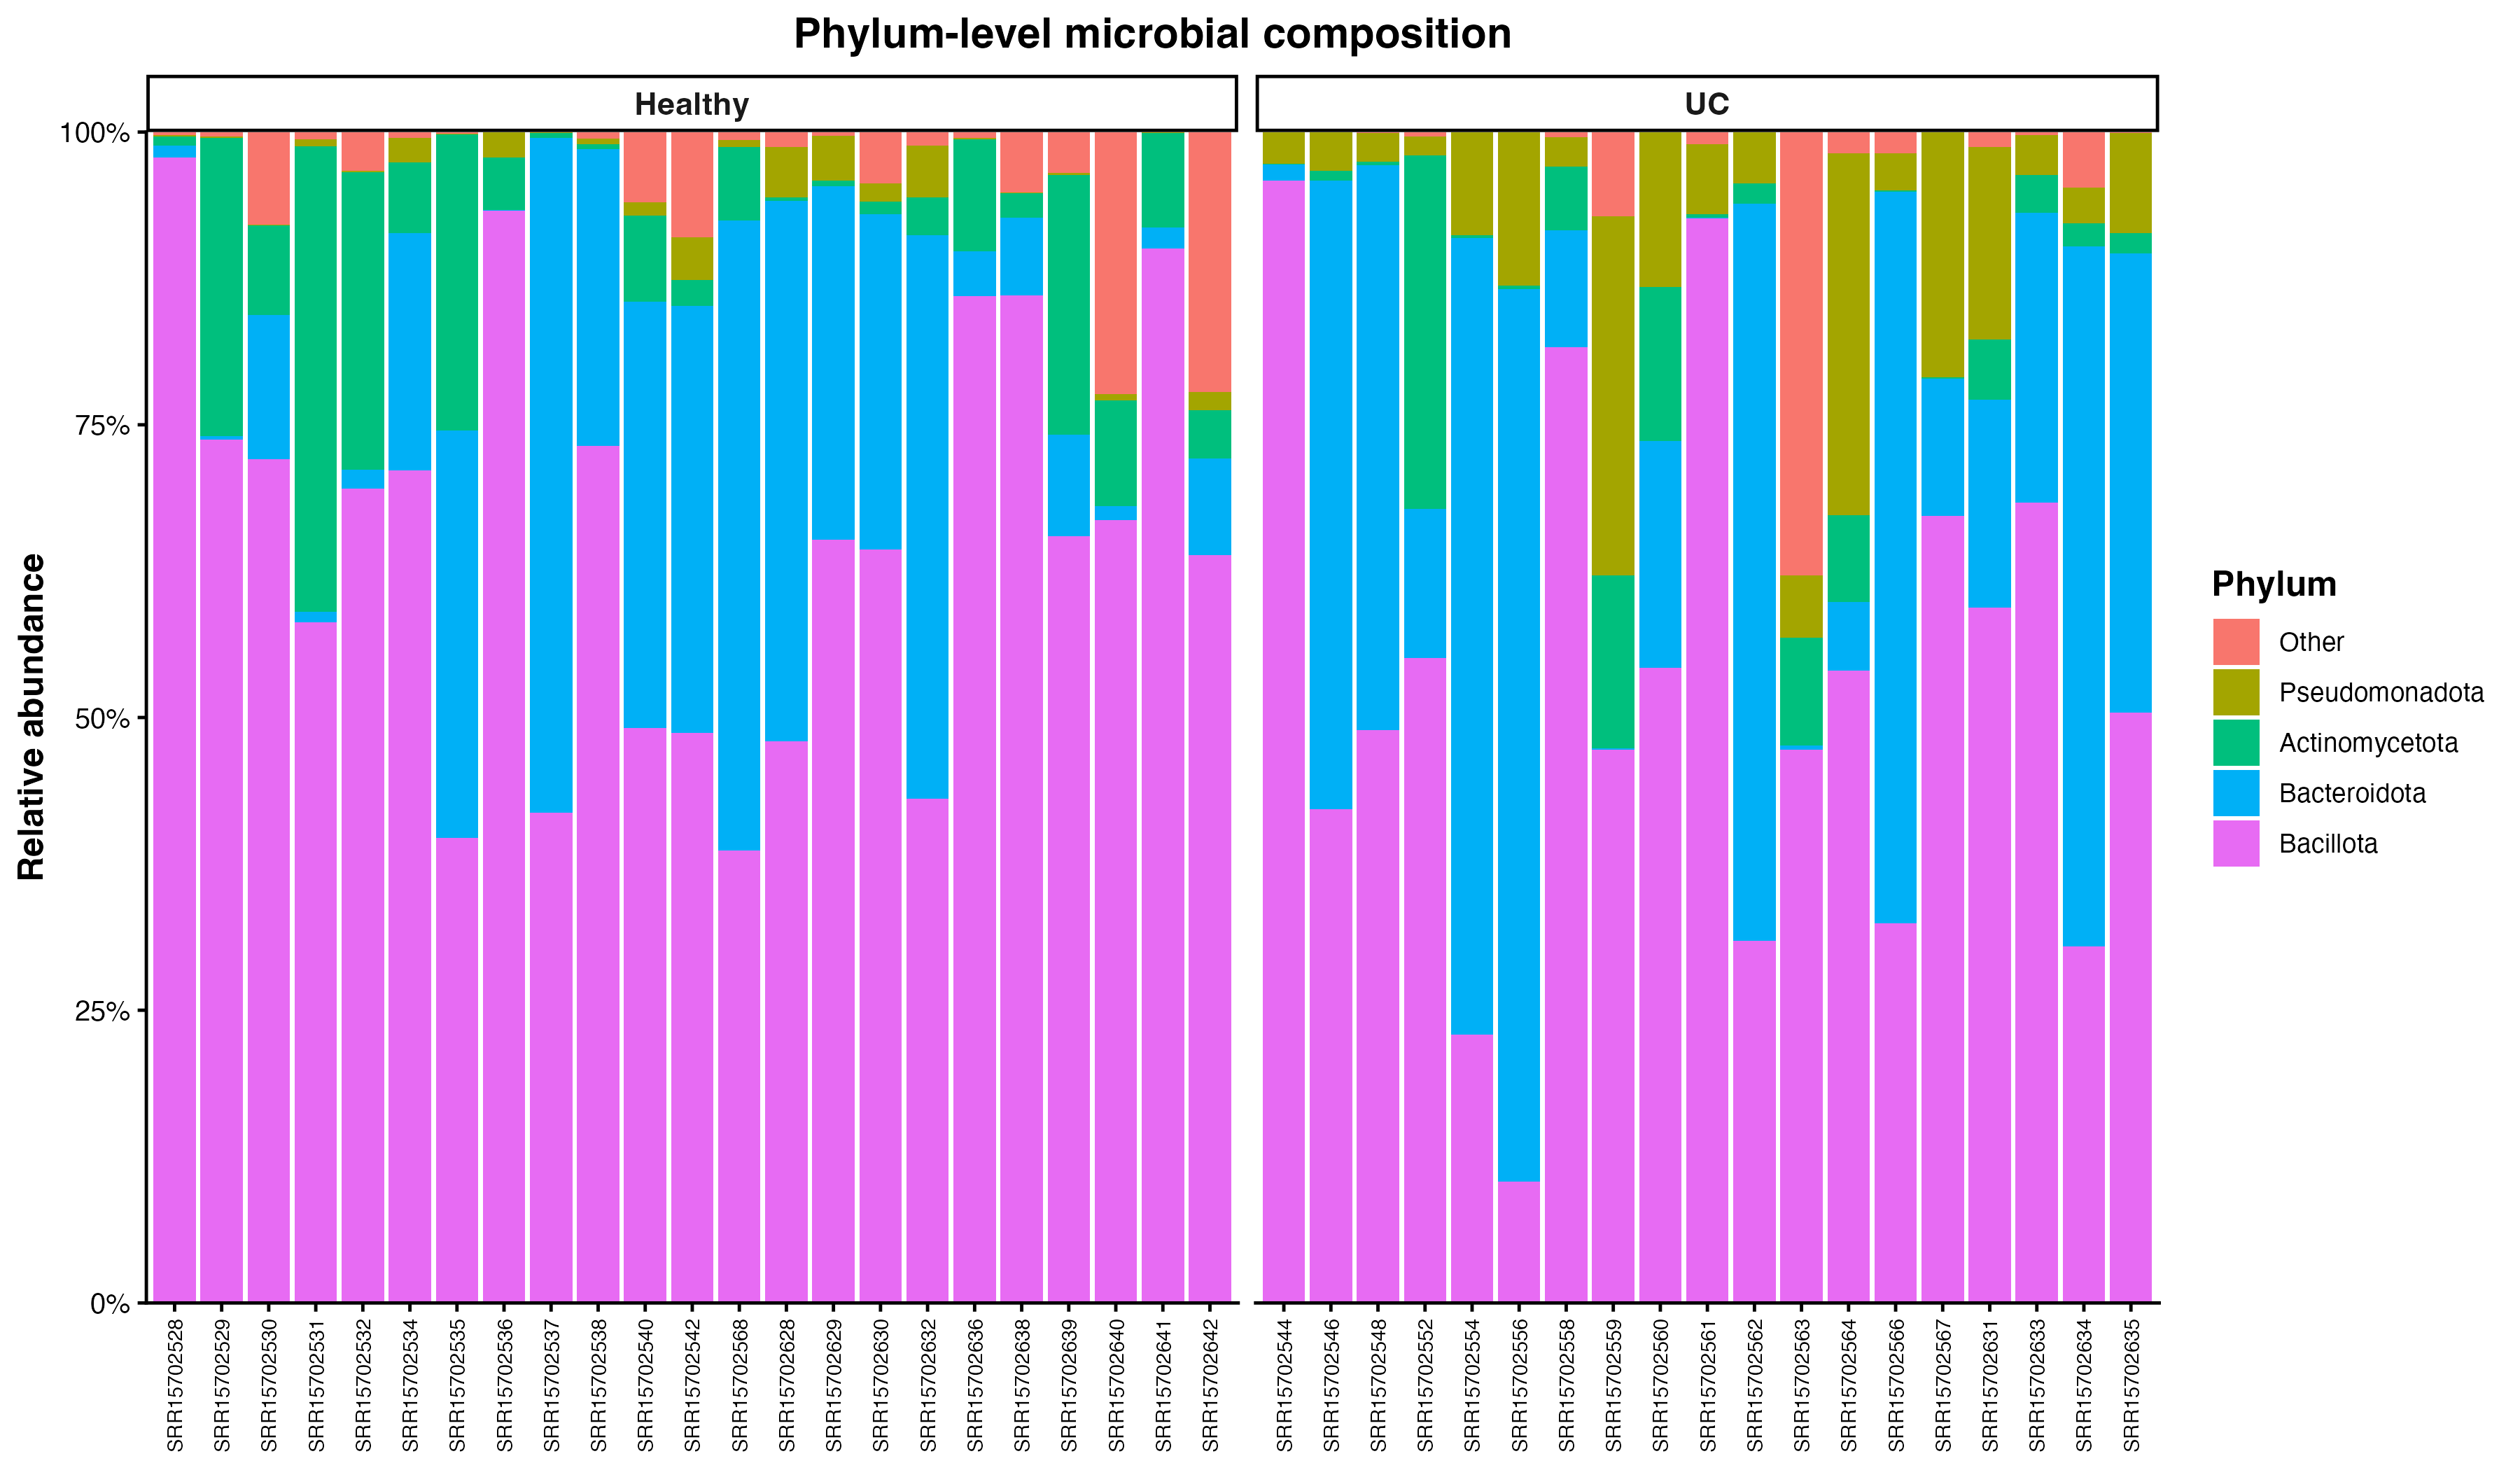
\includegraphics[width=1\linewidth,height=\textheight,keepaspectratio]{../results/plot/phyloseq_beta_alpha/phylum_composition.png}

}

\caption{\label{fig-phylum}Phylum-level composition of each sample,
grouped by clinical status. Phyla below 2\% mean relative abundance are
grouped as `Other'.}

\end{figure}%

\begin{longtable}[]{@{}
  >{\raggedright\arraybackslash}p{(\linewidth - 4\tabcolsep) * \real{0.3425}}
  >{\raggedleft\arraybackslash}p{(\linewidth - 4\tabcolsep) * \real{0.3288}}
  >{\raggedleft\arraybackslash}p{(\linewidth - 4\tabcolsep) * \real{0.3288}}@{}}
\caption{Mean phylum-level relative abundance by
group.}\label{tbl-phyla}\tabularnewline
\toprule\noalign{}
\begin{minipage}[b]{\linewidth}\raggedright
Phylum
\end{minipage} & \begin{minipage}[b]{\linewidth}\raggedleft
Healthy, mean relative abundance (\%)
\end{minipage} & \begin{minipage}[b]{\linewidth}\raggedleft
UC, mean relative abundance (\%)
\end{minipage} \\
\midrule\noalign{}
\endfirsthead
\toprule\noalign{}
\begin{minipage}[b]{\linewidth}\raggedright
Phylum
\end{minipage} & \begin{minipage}[b]{\linewidth}\raggedleft
Healthy, mean relative abundance (\%)
\end{minipage} & \begin{minipage}[b]{\linewidth}\raggedleft
UC, mean relative abundance (\%)
\end{minipage} \\
\midrule\noalign{}
\endhead
\bottomrule\noalign{}
\endlastfoot
Bacillota & 65.5 & 52.2 \\
Bacteroidota & 20.2 & 30.2 \\
Actinomycetota & 9.21 & 5.06 \\
Pseudomonadota & 1.21 & 9.49 \\
\end{longtable}

\subsection{Alpha diversity}\label{alpha-diversity}

Shannon diversity was lower in UC samples (median 2.442, IQR
2.031--2.686) than in healthy samples (median 2.693, IQR 2.564--3.044);
Wilcoxon p = 0.00205 (Figure~\ref{fig-shannon}).

\begin{figure}[H]

\centering{

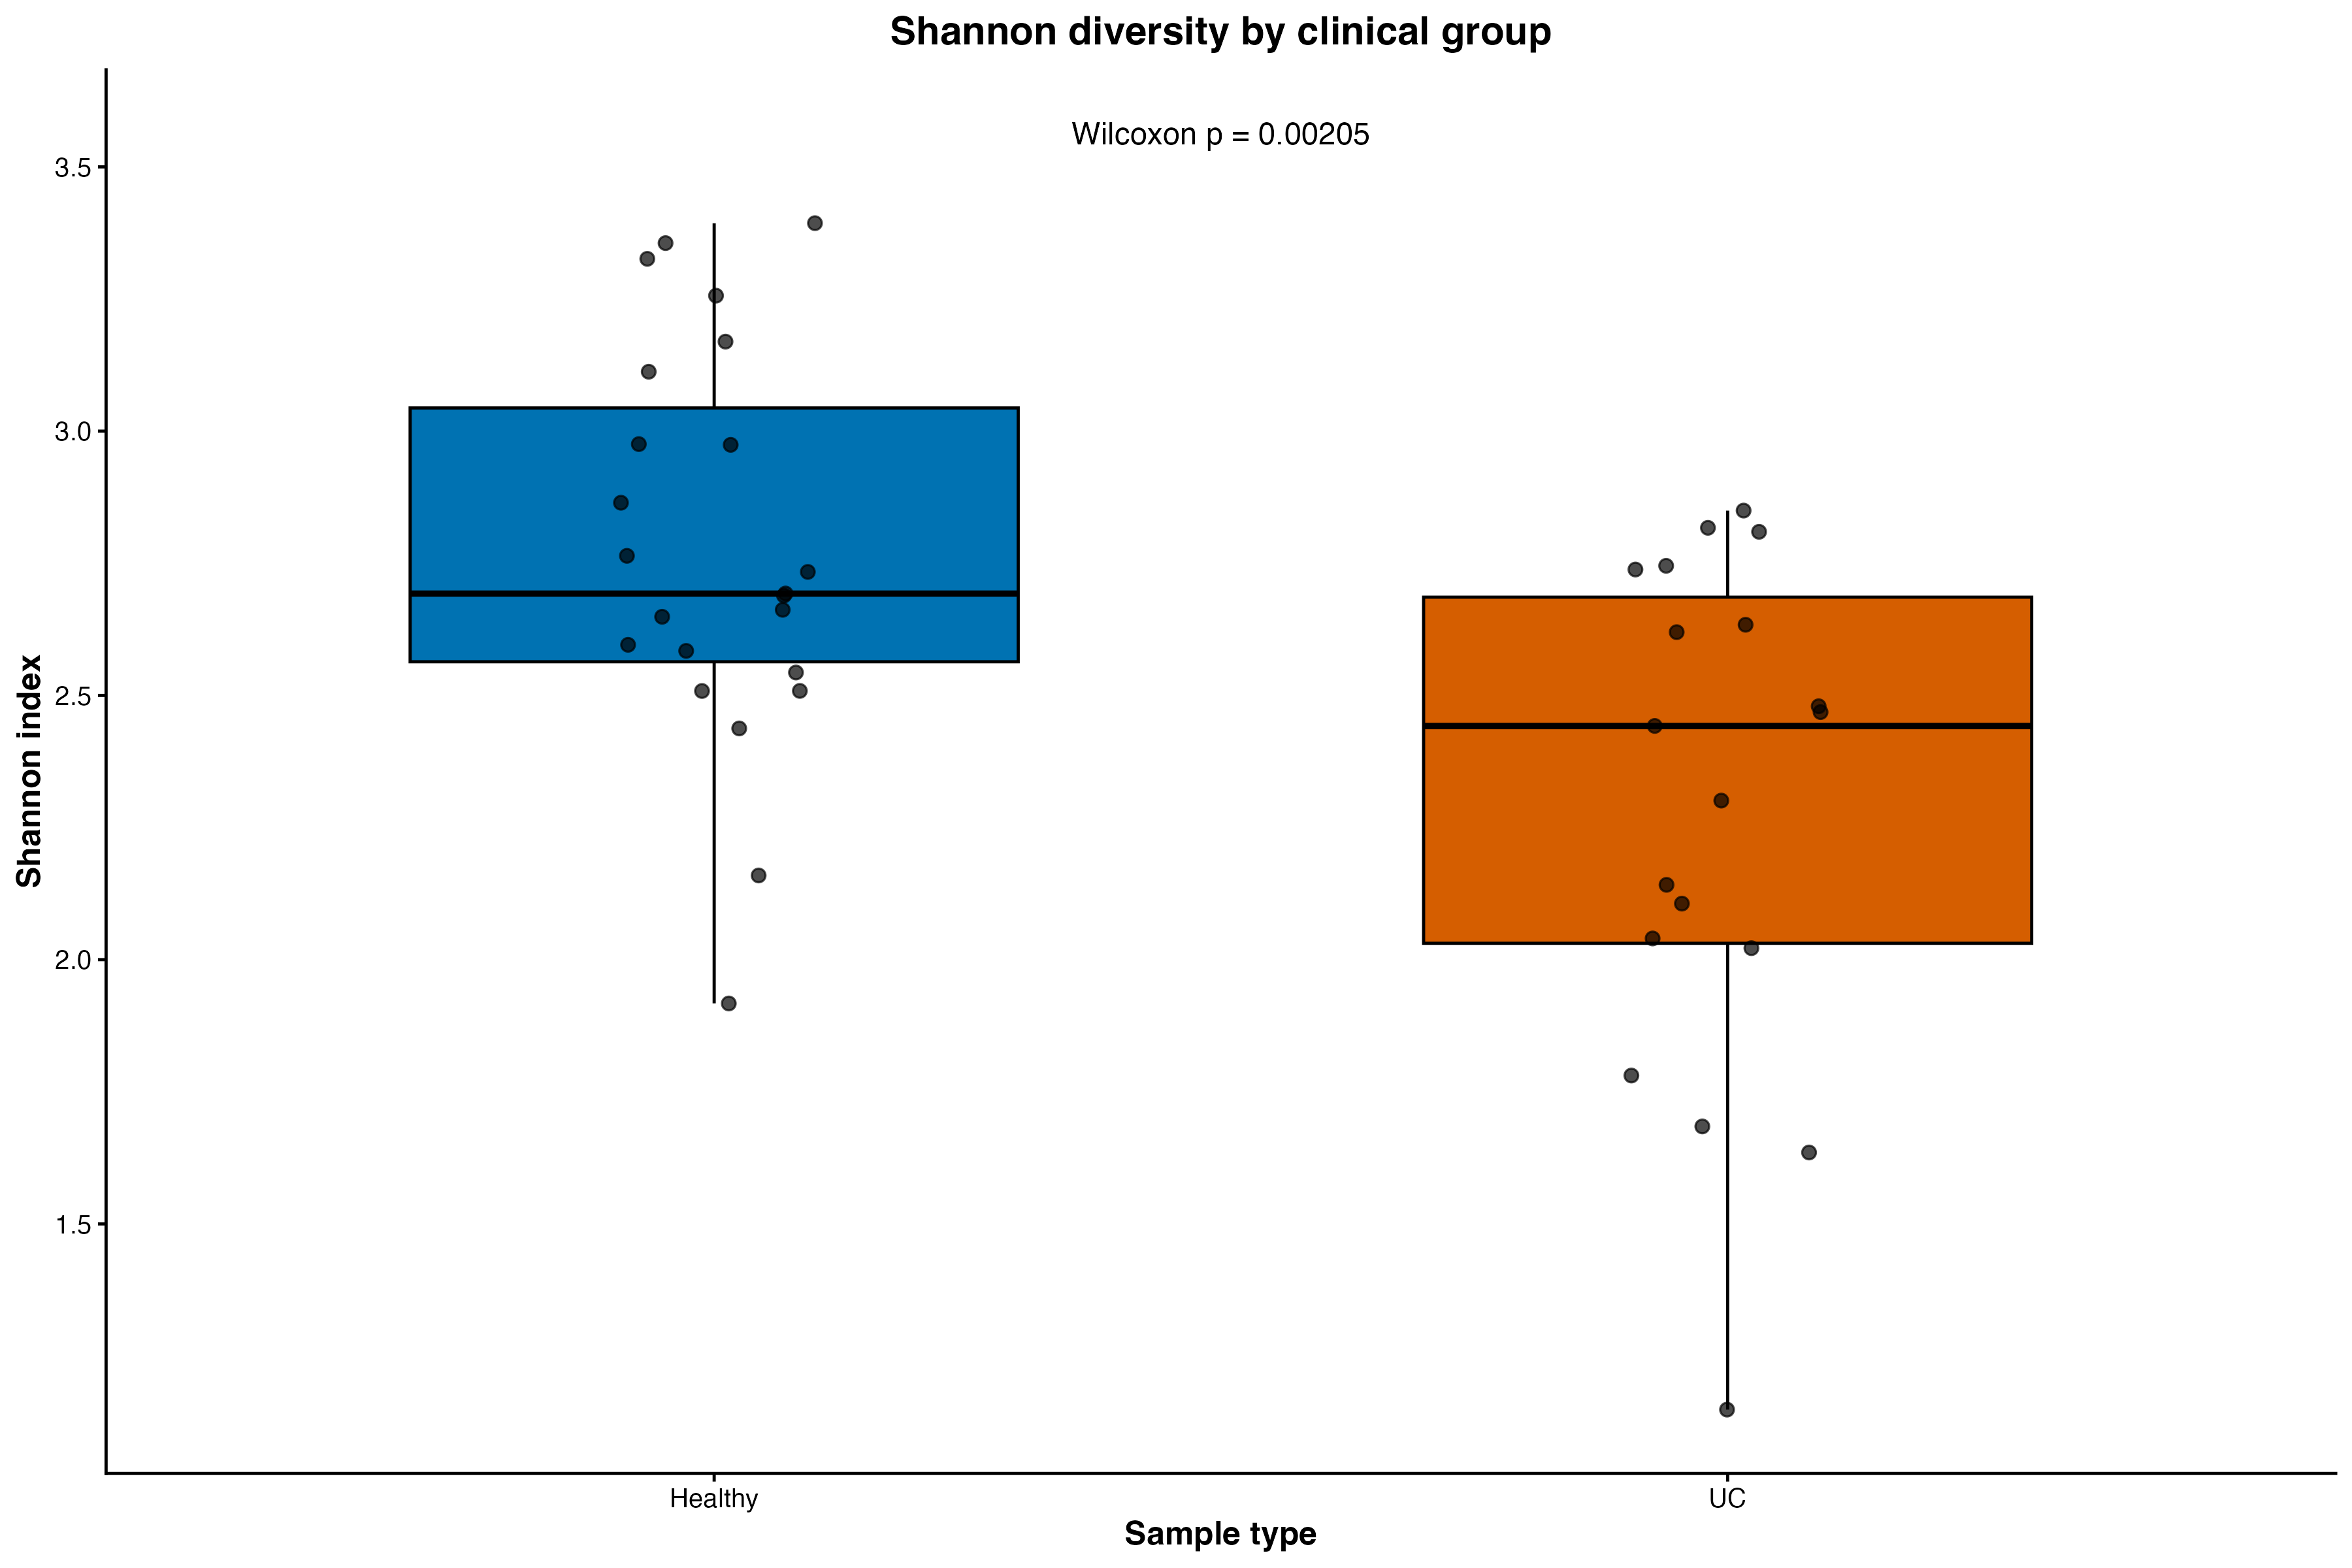
\includegraphics[width=1\linewidth,height=\textheight,keepaspectratio]{../results/plot/phyloseq_beta_alpha/alpha/shannon_diversity_by_sample_type.png}

}

\caption{\label{fig-shannon}Genus-level Shannon diversity by clinical
group (Wilcoxon rank-sum test).}

\end{figure}%

In the linear model adjusted for age and gender (Table~\ref{tbl-lm}), UC
was associated with a 0.804-fold change in Shannon diversity relative to
healthy samples (95\% CI 0.715--0.904; p = 0.000570). Age was not
associated with diversity (p = 0.653). Male gender showed a borderline,
non-significant association with higher diversity (fold change 1.12; p =
0.0519).

\begin{longtable}[]{@{}
  >{\raggedright\arraybackslash}p{(\linewidth - 8\tabcolsep) * \real{0.2000}}
  >{\raggedleft\arraybackslash}p{(\linewidth - 8\tabcolsep) * \real{0.2000}}
  >{\raggedleft\arraybackslash}p{(\linewidth - 8\tabcolsep) * \real{0.2000}}
  >{\raggedleft\arraybackslash}p{(\linewidth - 8\tabcolsep) * \real{0.2000}}
  >{\raggedleft\arraybackslash}p{(\linewidth - 8\tabcolsep) * \real{0.2000}}@{}}
\caption{Linear model of log(Shannon) on disease status, age and gender
(R² = 0.314).}\label{tbl-lm}\tabularnewline
\toprule\noalign{}
\begin{minipage}[b]{\linewidth}\raggedright
Term
\end{minipage} & \begin{minipage}[b]{\linewidth}\raggedleft
Estimate (log scale)
\end{minipage} & \begin{minipage}[b]{\linewidth}\raggedleft
95\% CI
\end{minipage} & \begin{minipage}[b]{\linewidth}\raggedleft
Fold change
\end{minipage} & \begin{minipage}[b]{\linewidth}\raggedleft
p-value
\end{minipage} \\
\midrule\noalign{}
\endfirsthead
\toprule\noalign{}
\begin{minipage}[b]{\linewidth}\raggedright
Term
\end{minipage} & \begin{minipage}[b]{\linewidth}\raggedleft
Estimate (log scale)
\end{minipage} & \begin{minipage}[b]{\linewidth}\raggedleft
95\% CI
\end{minipage} & \begin{minipage}[b]{\linewidth}\raggedleft
Fold change
\end{minipage} & \begin{minipage}[b]{\linewidth}\raggedleft
p-value
\end{minipage} \\
\midrule\noalign{}
\endhead
\bottomrule\noalign{}
\endlastfoot
UC vs Healthy & -0.2182 & -0.336 to -0.101 & 0.804 & 0.000570 \\
Age (per year) & -0.0038 & -0.021 to 0.013 & 0.996 & 0.653 \\
Gender (male vs female) & 0.1159 & -0.001 to 0.233 & 1.123 & 0.0519 \\
\end{longtable}

\subsubsection{Robustness to sequencing
depth}\label{robustness-to-sequencing-depth}

Library size was moderately correlated with Shannon diversity (Spearman
ρ = 0.425, p = 0.00499) and strongly correlated with the number of
observed genera (ρ = 0.734, p \textless{} 0.001). When log10 library
size was added to the model, the UC effect was attenuated but remained
statistically significant (estimate = -0.181, p = 0.00984). Rarefaction
curves (Figure~\ref{fig-rarecurve}) reached a plateau for most samples.

\begin{figure}[H]

\centering{

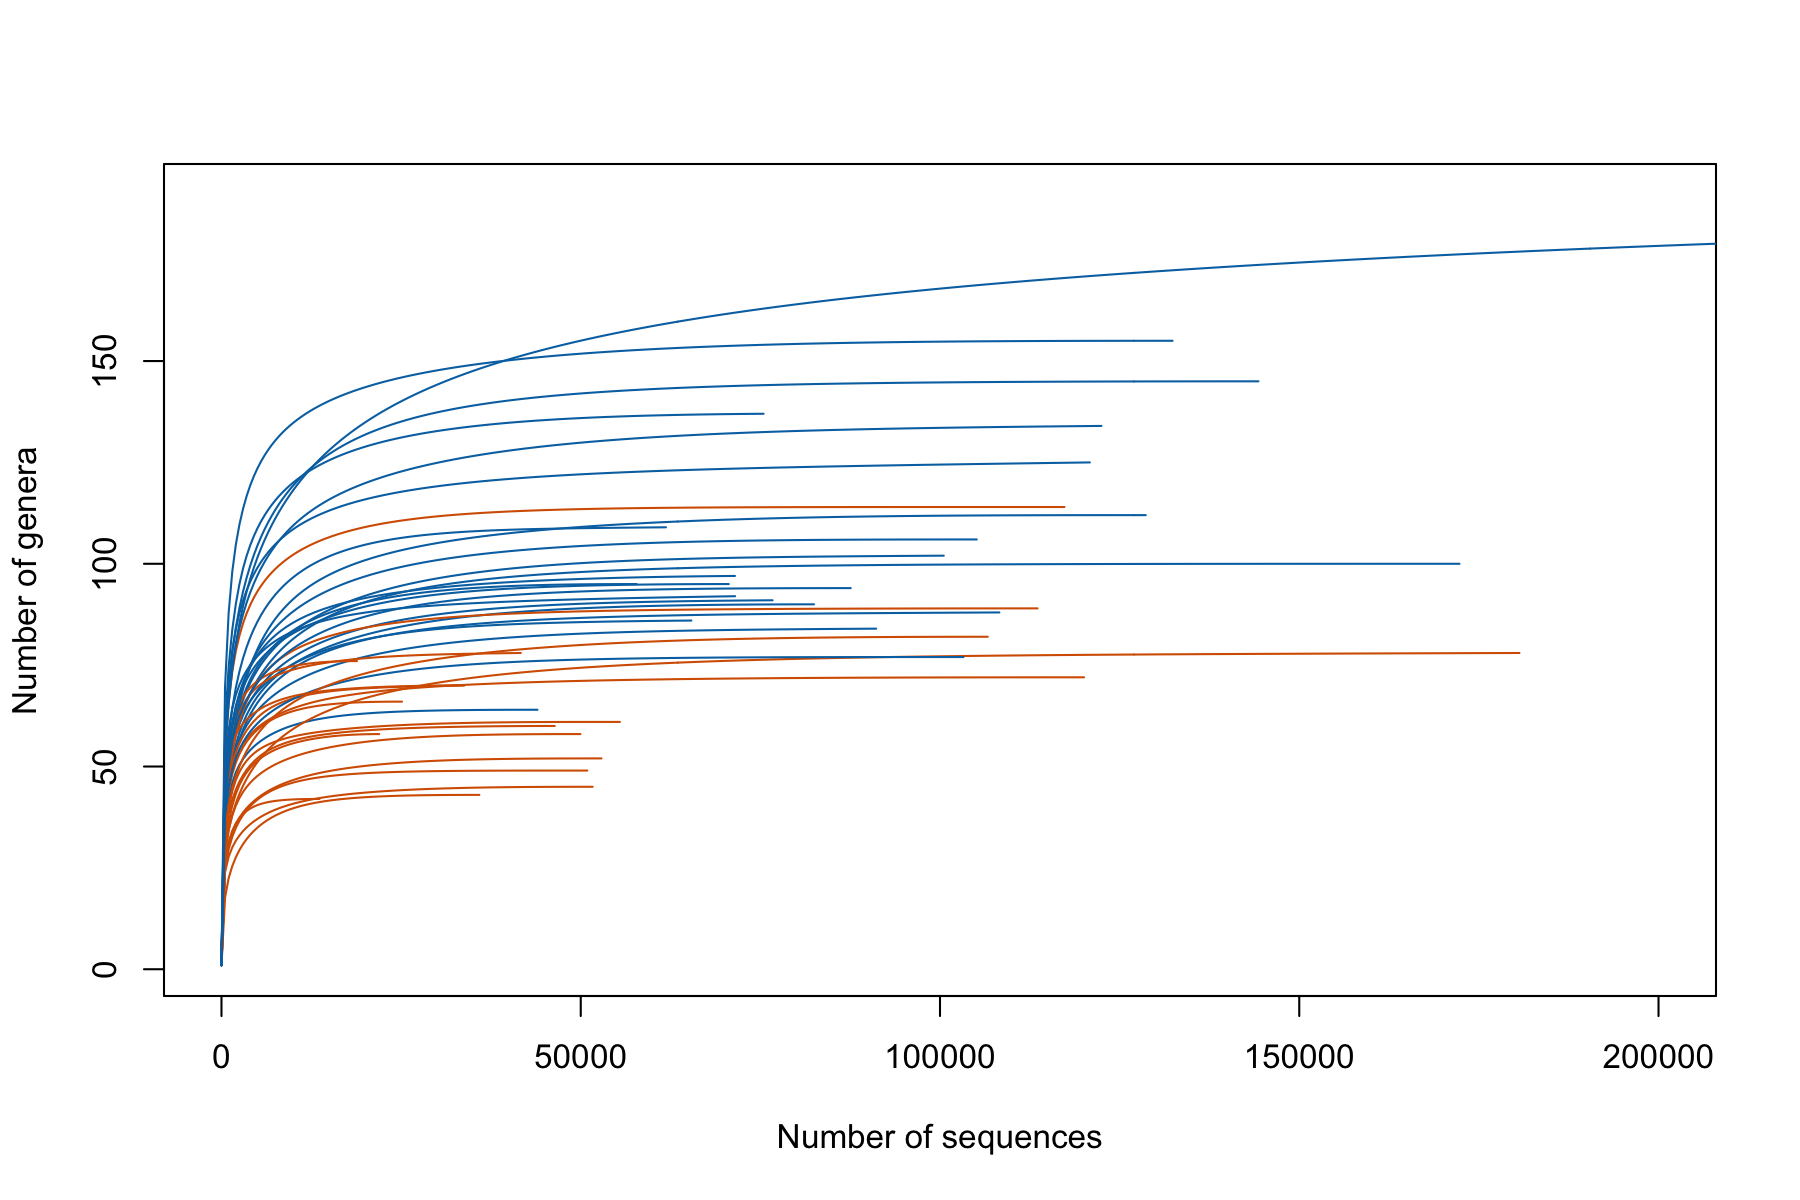
\includegraphics[width=1\linewidth,height=\textheight,keepaspectratio]{../results/plot/phyloseq_beta_alpha/rarefaction_curves_genus.png}

}

\caption{\label{fig-rarecurve}Genus-level rarefaction curves (blue:
Healthy, orange: UC).}

\end{figure}%

The group comparison was repeated after rarefaction at six depths
(Figure~\ref{fig-rarefaction}, Table~\ref{tbl-rare}). Mean Shannon
diversity was slightly lower at 1,000 reads and stable from 5,000 reads
upward, and the difference between Healthy and UC was preserved at every
depth (Wilcoxon p = 0.00205 at all depths; the test depends only on the
ranking of samples, which did not change). All samples have at least
13,639 reads, so the comparisons at 1,000, 5,000 and 10,000 reads are
fully rarefied; at 30,000, 50,000 and 100,000 reads, 4, 11 and 26
samples fall below the target depth and are kept with all their reads,
so those panels are only partly rarefied.

\begin{figure}[H]

\centering{

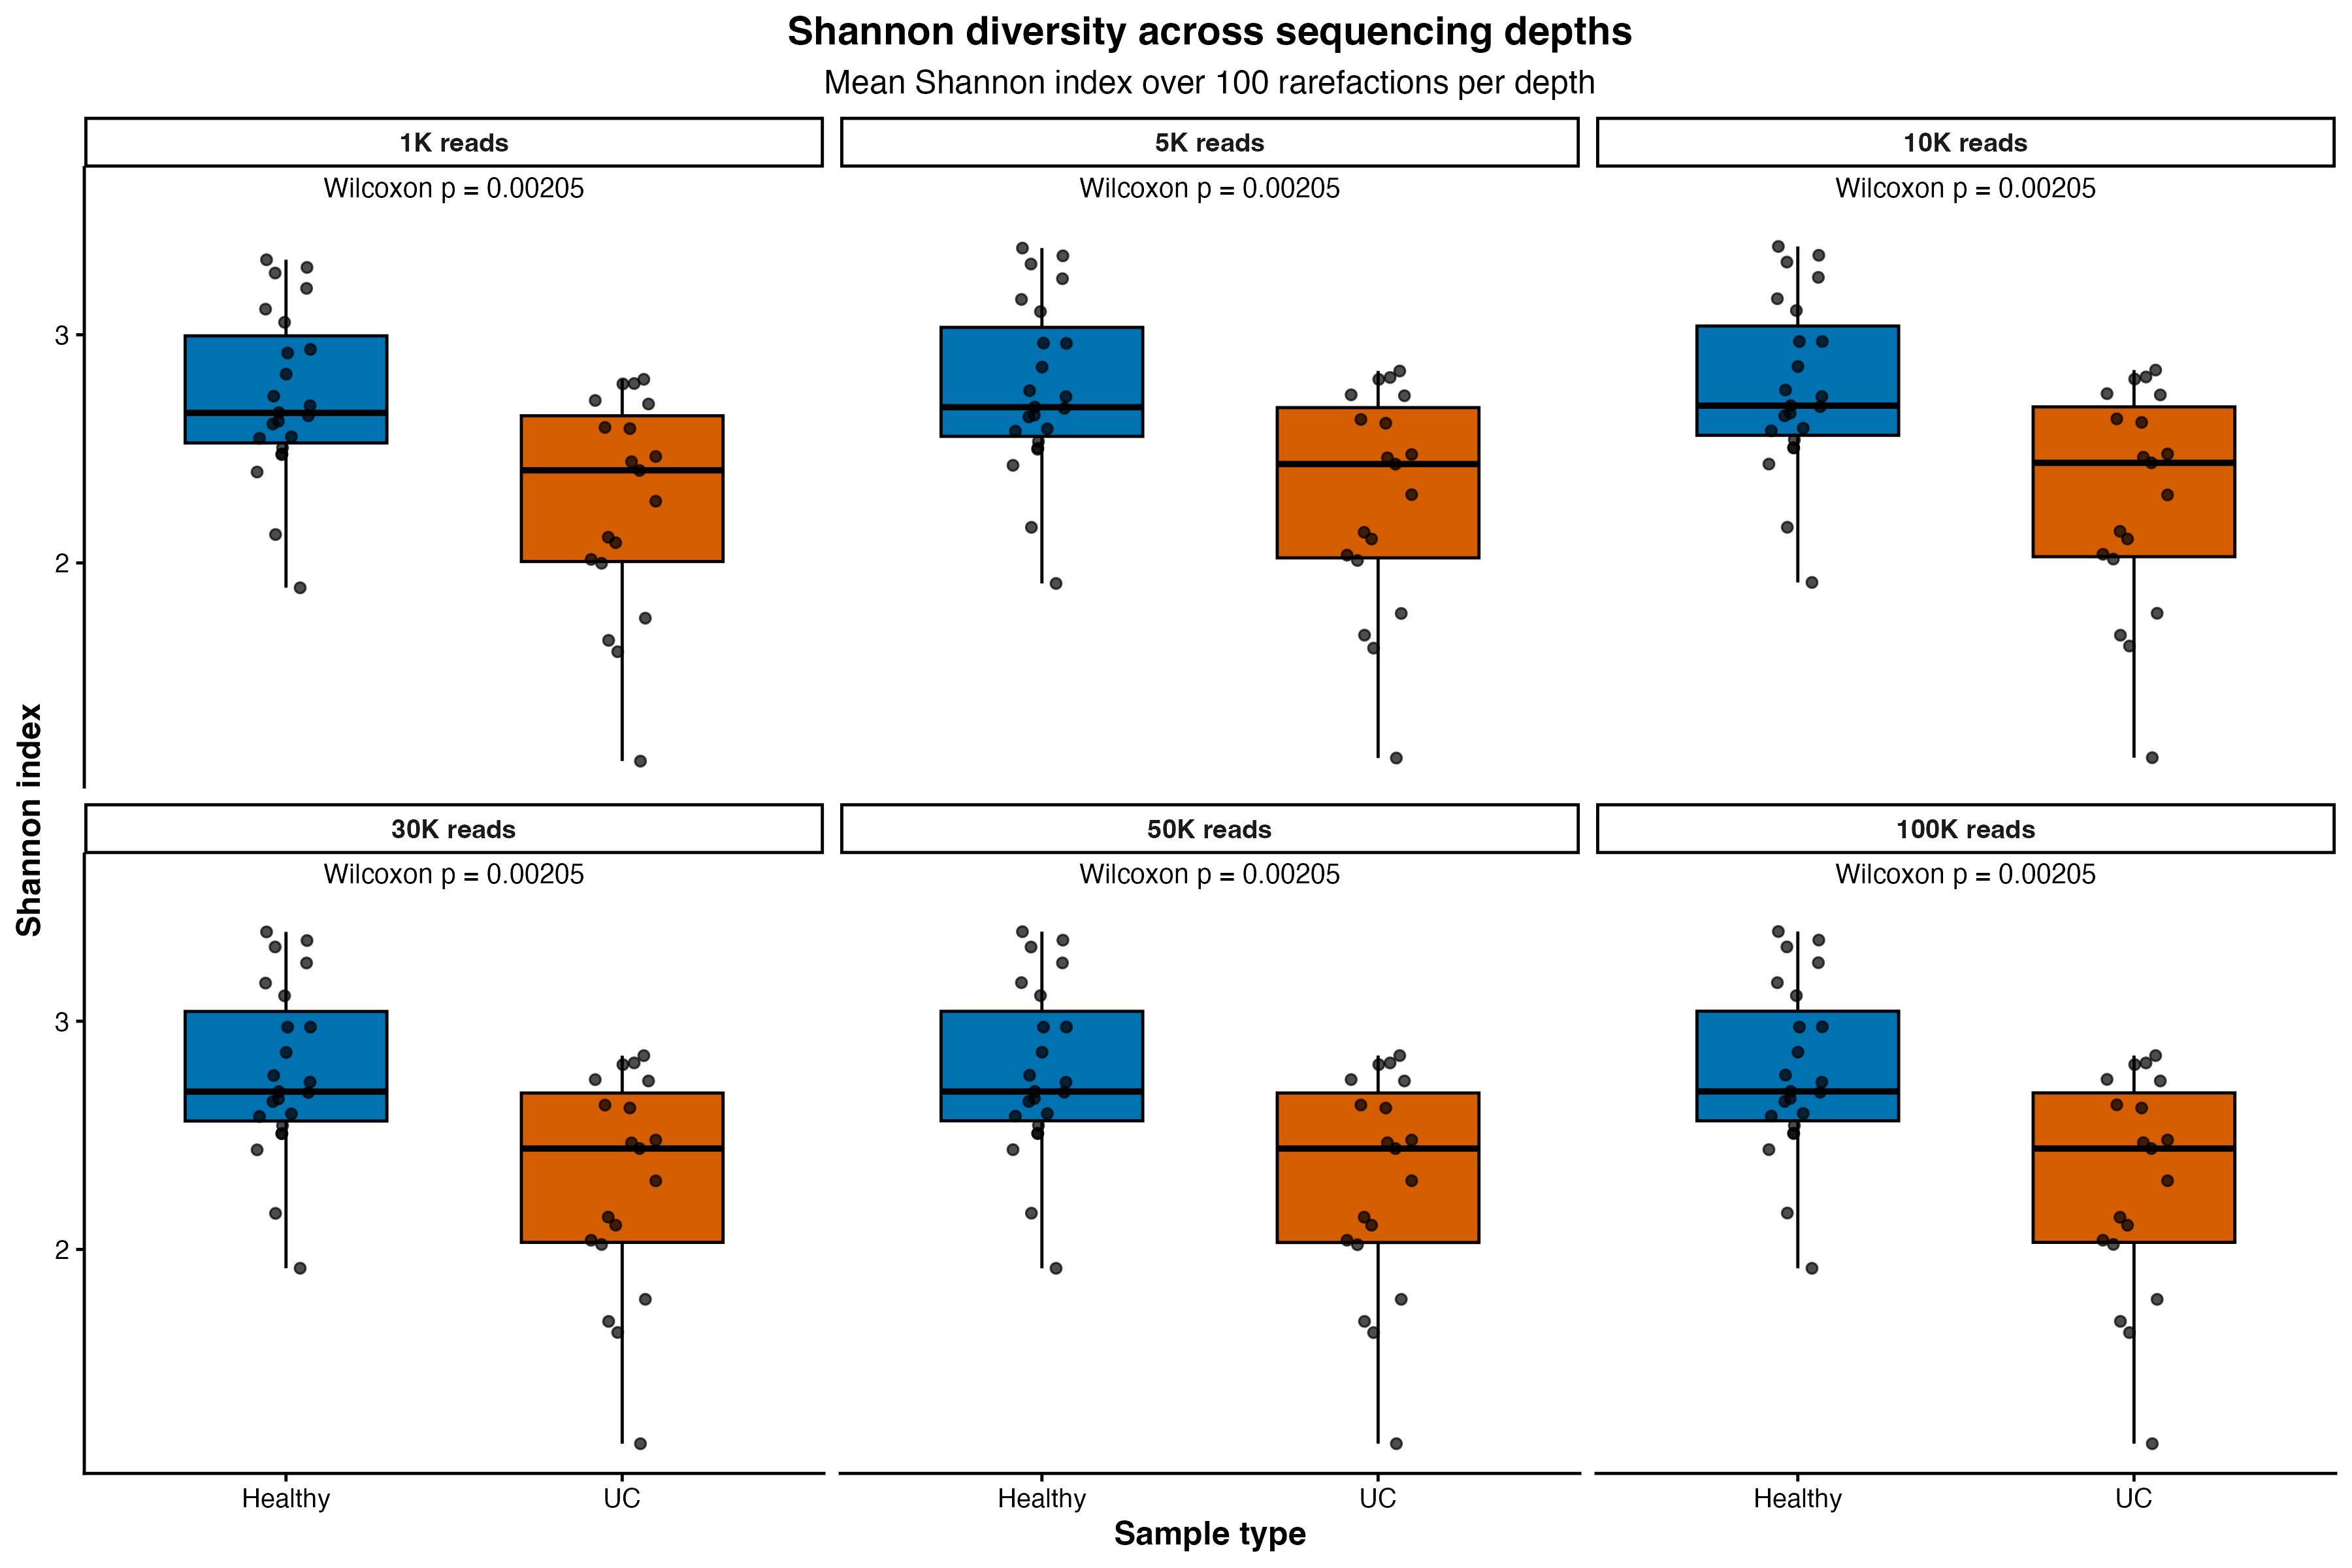
\includegraphics[width=1\linewidth,height=\textheight,keepaspectratio]{../results/plot/phyloseq_beta_alpha/alpha/shannon_rarefaction_sensitivity.png}

}

\caption{\label{fig-rarefaction}Shannon diversity by clinical group at
increasing rarefaction depths. For each sample, the index was calculated
on each of 100 rarefied tables and averaged.}

\end{figure}%

\begin{longtable}[]{@{}
  >{\raggedleft\arraybackslash}p{(\linewidth - 4\tabcolsep) * \real{0.2055}}
  >{\raggedleft\arraybackslash}p{(\linewidth - 4\tabcolsep) * \real{0.5479}}
  >{\raggedleft\arraybackslash}p{(\linewidth - 4\tabcolsep) * \real{0.2466}}@{}}
\caption{Group comparison of Shannon diversity across rarefaction
depths.}\label{tbl-rare}\tabularnewline
\toprule\noalign{}
\begin{minipage}[b]{\linewidth}\raggedleft
Depth (reads)
\end{minipage} & \begin{minipage}[b]{\linewidth}\raggedleft
Samples below depth (retained in full)
\end{minipage} & \begin{minipage}[b]{\linewidth}\raggedleft
Wilcoxon p-value
\end{minipage} \\
\midrule\noalign{}
\endfirsthead
\toprule\noalign{}
\begin{minipage}[b]{\linewidth}\raggedleft
Depth (reads)
\end{minipage} & \begin{minipage}[b]{\linewidth}\raggedleft
Samples below depth (retained in full)
\end{minipage} & \begin{minipage}[b]{\linewidth}\raggedleft
Wilcoxon p-value
\end{minipage} \\
\midrule\noalign{}
\endhead
\bottomrule\noalign{}
\endlastfoot
1,000 & 0 & 0.00205 \\
5,000 & 0 & 0.00205 \\
10,000 & 0 & 0.00205 \\
30,000 & 4 & 0.00205 \\
50,000 & 11 & 0.00205 \\
100,000 & 26 & 0.00205 \\
\end{longtable}

\subsection{Beta diversity}\label{beta-diversity}

The first two PCoA axes of the genus-level Bray-Curtis distances
explained 30.3\% and 13.1\% of the variation (Figure~\ref{fig-pcoa}).
Samples partly separated by clinical group.

\begin{figure}[H]

\centering{

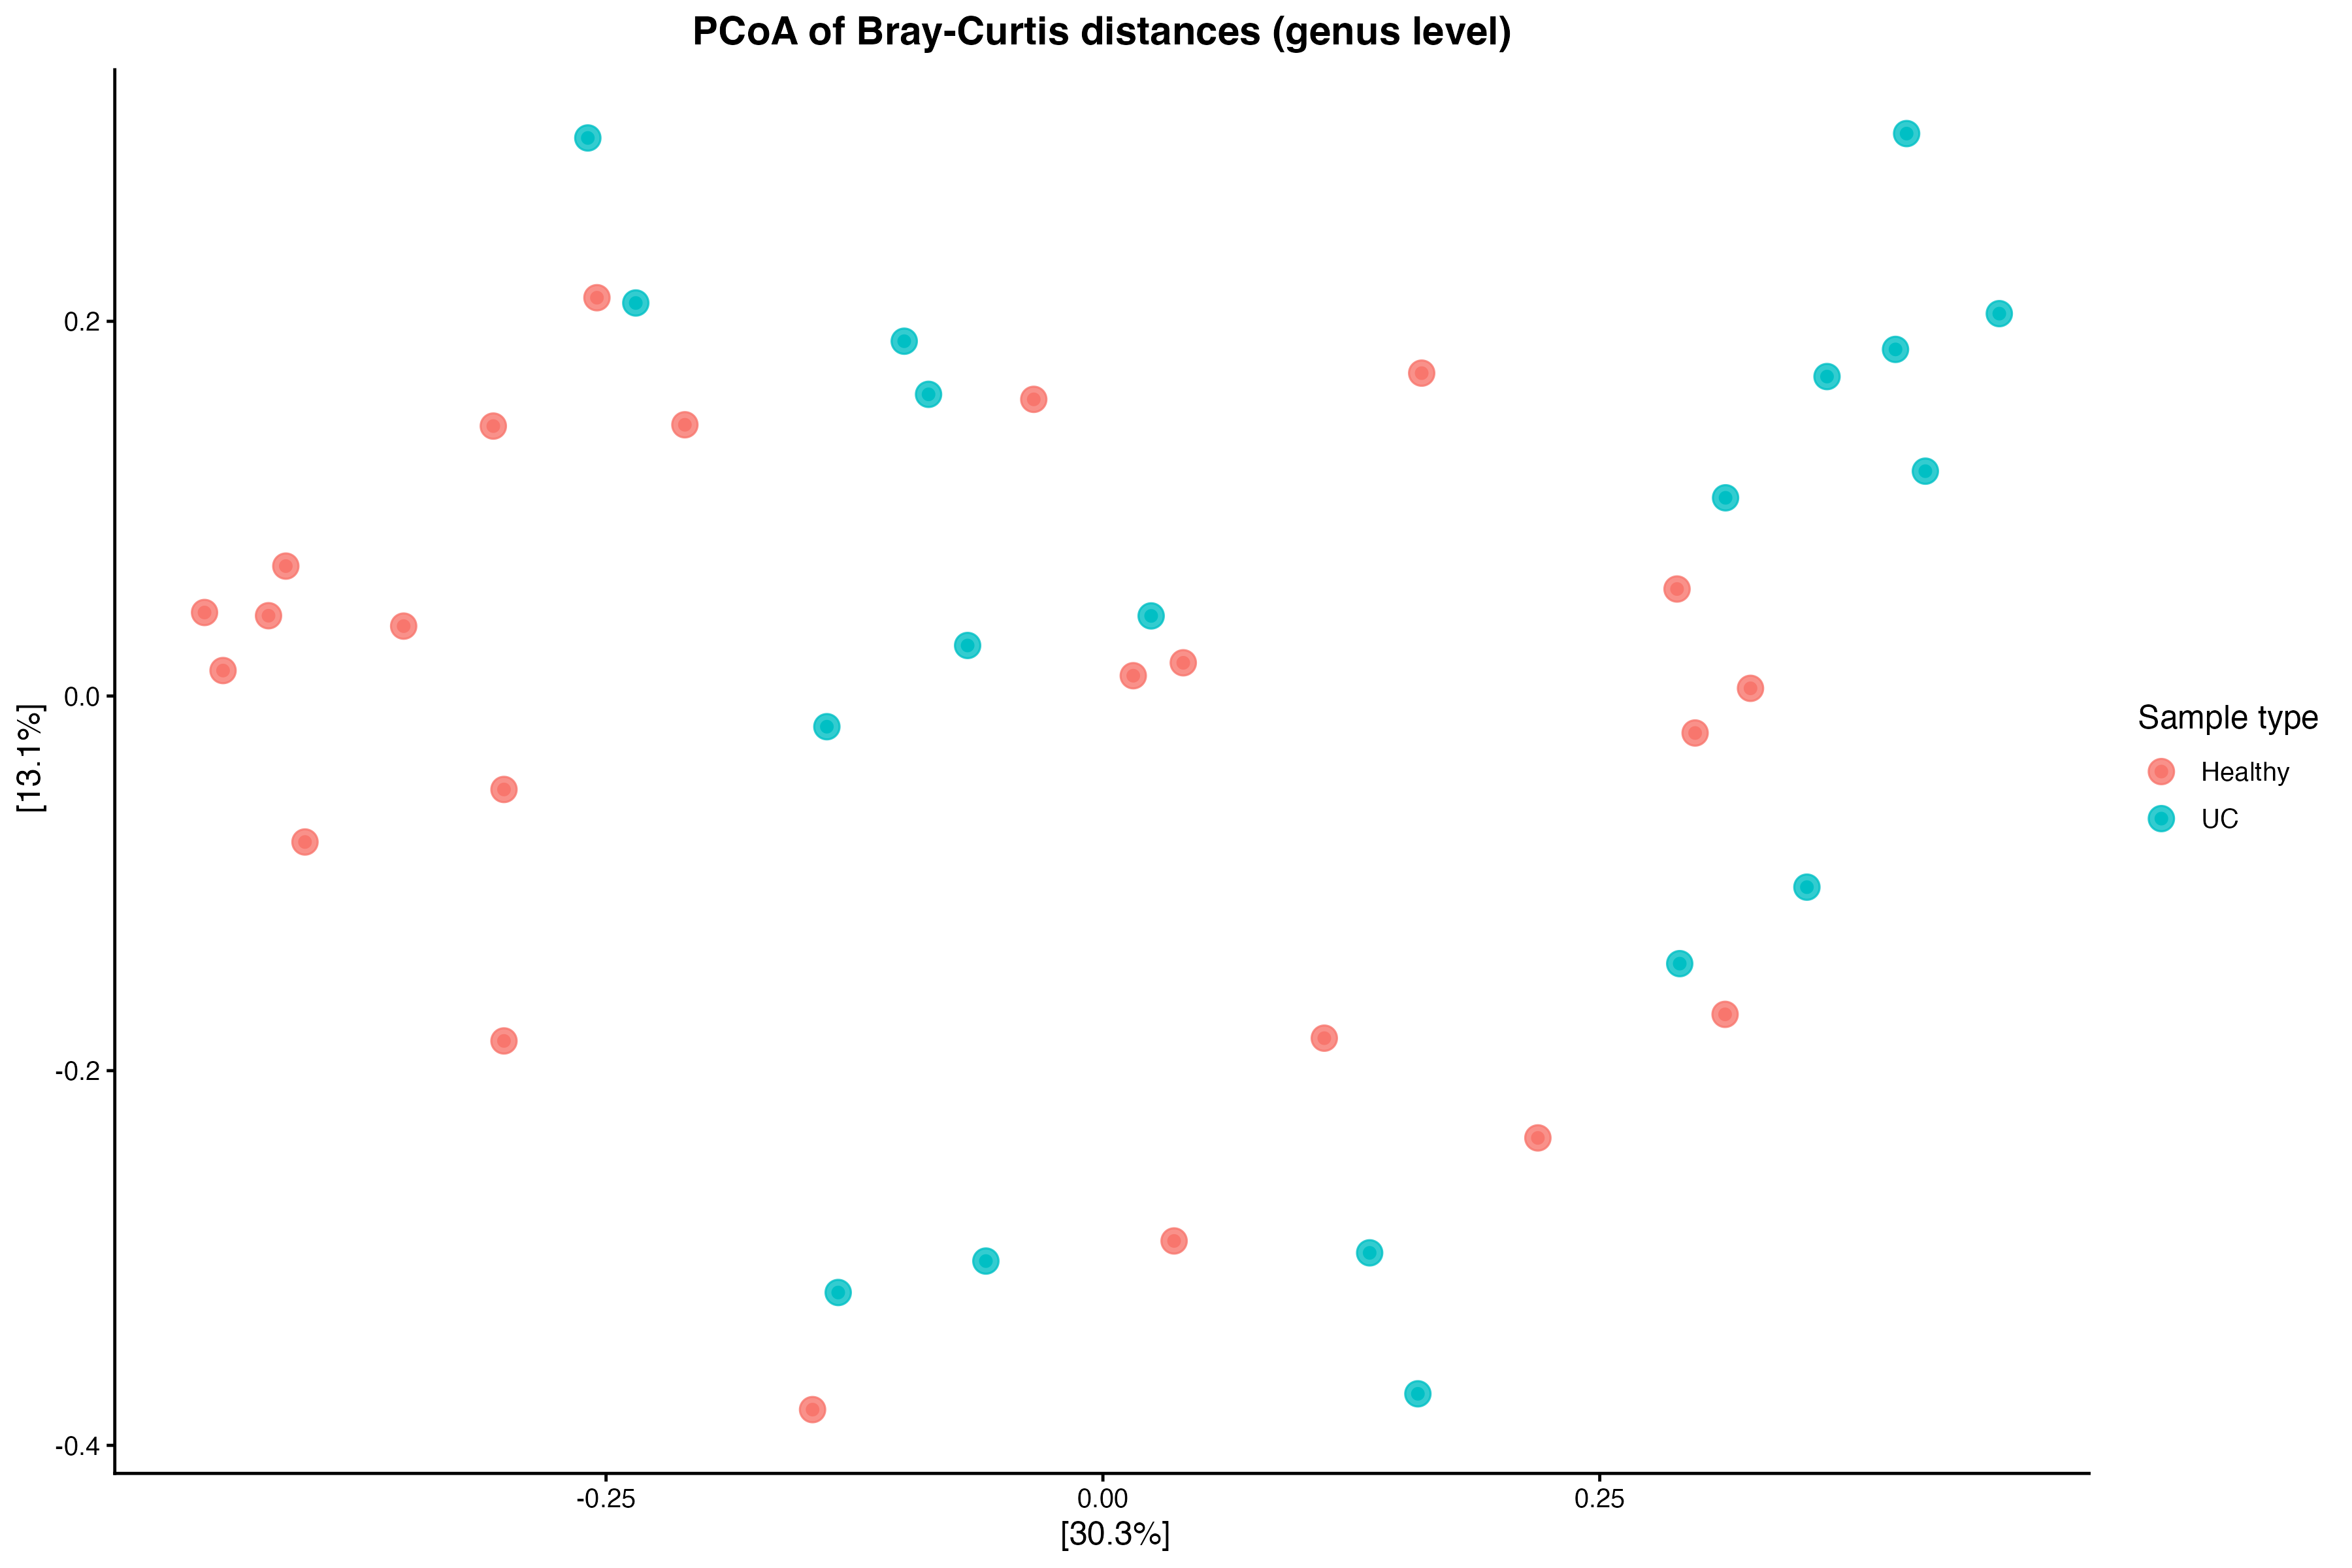
\includegraphics[width=1\linewidth,height=\textheight,keepaspectratio]{../results/plot/phyloseq_beta_alpha/beta/pcoa_bray_curtis_genus.png}

}

\caption{\label{fig-pcoa}PCoA of genus-level Bray-Curtis
dissimilarities, coloured by clinical group.}

\end{figure}%

PERMANOVA with marginal effects (Table~\ref{tbl-permanova}) showed that
disease status explained 9.70\% of the variation (pseudo-F = 4.44, p =
0.001) after adjustment for age and gender. Age was not significantly
associated with community composition (R² = 4.11\%, p = 0.071), and
neither was gender (R² = 3.57\%, p = 0.104).

\begin{longtable}[]{@{}lrrrrr@{}}
\caption{PERMANOVA on genus-level Bray-Curtis dissimilarities, marginal
effects, 999 permutations.}\label{tbl-permanova}\tabularnewline
\toprule\noalign{}
Term & df & Sum of squares & R² & pseudo-F & p-value \\
\midrule\noalign{}
\endfirsthead
\toprule\noalign{}
Term & df & Sum of squares & R² & pseudo-F & p-value \\
\midrule\noalign{}
\endhead
\bottomrule\noalign{}
\endlastfoot
Disease status & 1 & 1.0468 & 0.0970 & 4.4435 & 0.001 \\
Age & 1 & 0.4429 & 0.0411 & 1.8802 & 0.071 \\
Gender & 1 & 0.3849 & 0.0357 & 1.6336 & 0.104 \\
Residual & 38 & 8.9522 & 0.8297 & --- & --- \\
\end{longtable}

Because PERMANOVA is sensitive to differences in within-group
variability, homogeneity of multivariate dispersion was tested:
dispersion did not differ significantly between groups (F = 0.936, p =
0.329; Figure~\ref{fig-betadisper}), although UC samples show a visibly
wider spread and the power of this test is limited with 19 UC samples.

\begin{figure}[H]

\centering{

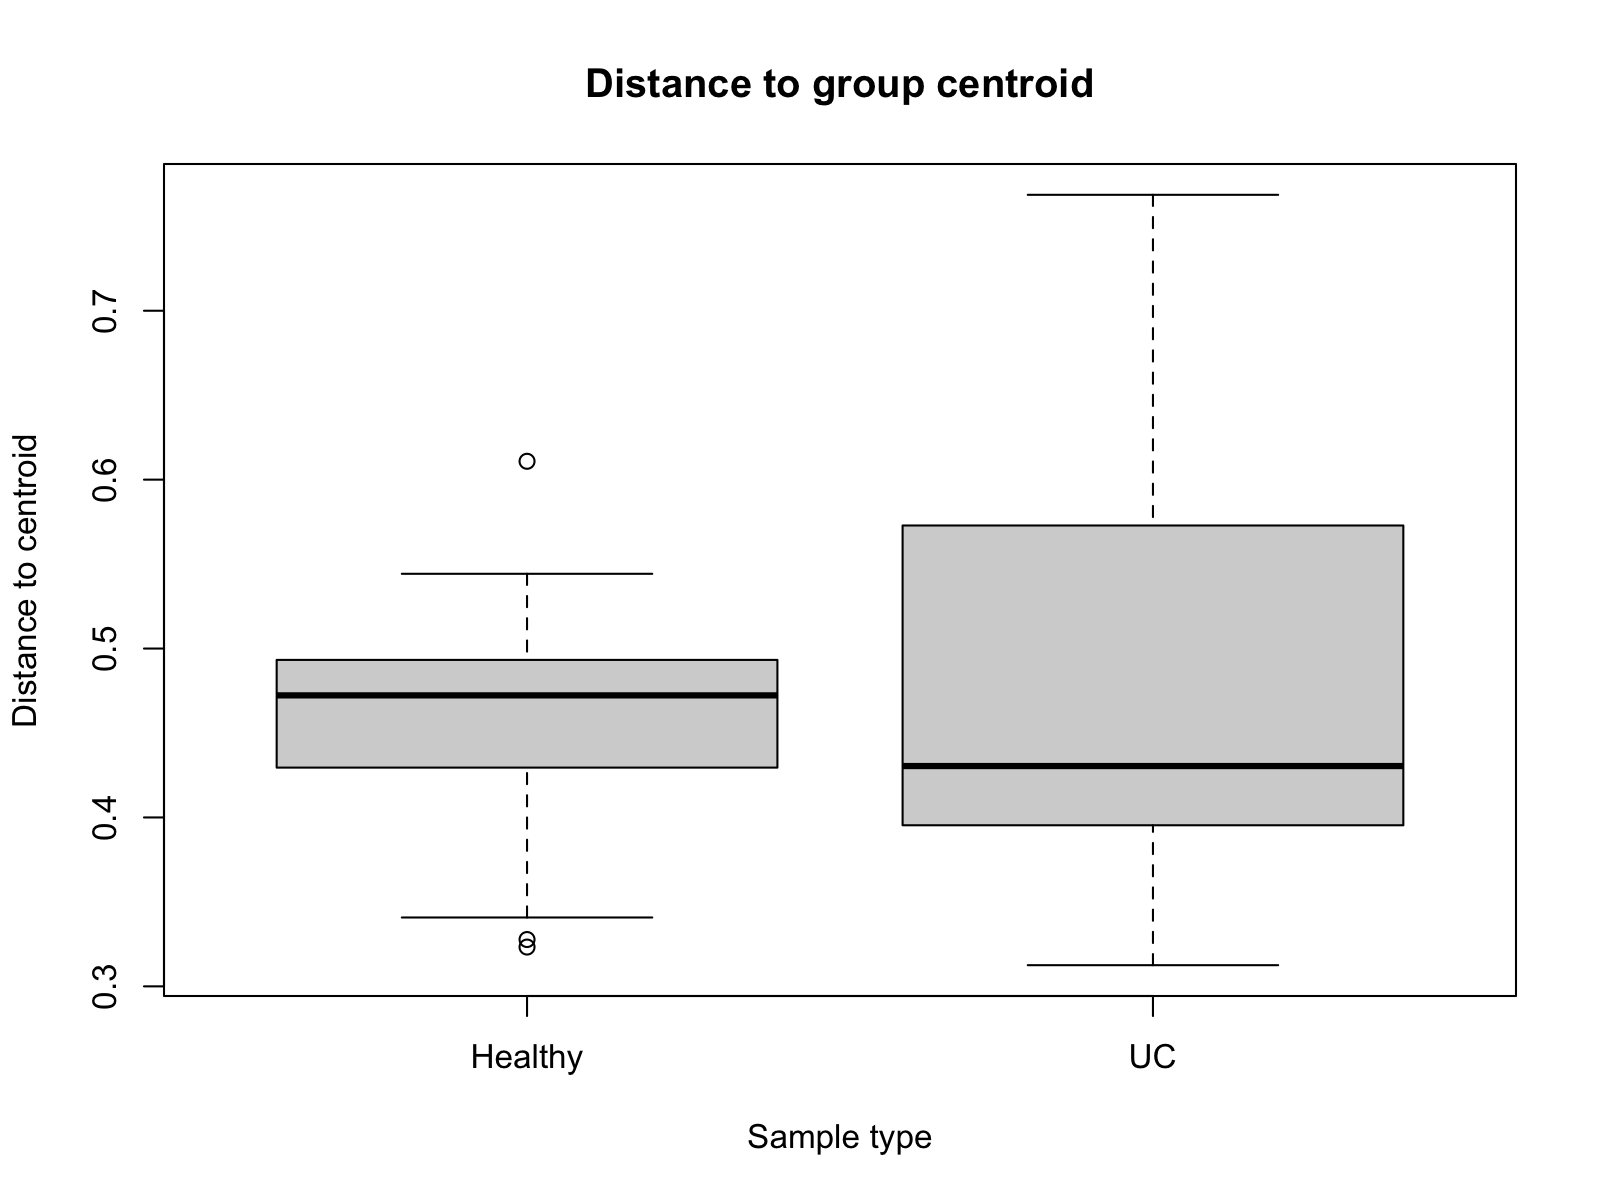
\includegraphics[width=1\linewidth,height=\textheight,keepaspectratio]{../results/plot/phyloseq_beta_alpha/beta/betadisper_boxplot.png}

}

\caption{\label{fig-betadisper}Distance to the group centroid
(Bray-Curtis) by clinical group.}

\end{figure}%

Multiple Regression on distance Matrices (Table~\ref{tbl-mrm}) gives a
complementary view, modelling pairwise dissimilarities. Healthy--UC
pairs were more dissimilar than Healthy--Healthy pairs (coefficient
0.0817, p = 0.007). UC--UC pairs had a positive coefficient of similar
magnitude (0.0600) that did not reach significance (p = 0.222); with 19
UC samples, the data therefore do not allow us to conclude whether UC
microbiomes are more heterogeneous among themselves than healthy ones.
The overall MRM model explained 4.88\% of the variation in pairwise
dissimilarities and was not significant (p = 0.122), so the Healthy--UC
coefficient should be read together with the PERMANOVA result.

\begin{longtable}[]{@{}lrr@{}}
\caption{MRM on genus-level Bray-Curtis dissimilarities, 999
permutations.}\label{tbl-mrm}\tabularnewline
\toprule\noalign{}
Predictor (pairwise) & Coefficient & p-value \\
\midrule\noalign{}
\endfirsthead
\toprule\noalign{}
Predictor (pairwise) & Coefficient & p-value \\
\midrule\noalign{}
\endhead
\bottomrule\noalign{}
\endlastfoot
Healthy--UC pair (vs Healthy--Healthy) & 0.0817 & 0.007 \\
UC--UC pair (vs Healthy--Healthy) & 0.0600 & 0.222 \\
Age difference & -0.0046 & 0.256 \\
Female--Male pair (vs Male--Male) & 0.0119 & 0.649 \\
Female--Female pair (vs Male--Male) & 0.0163 & 0.724 \\
\end{longtable}

\subsection{Differential abundance}\label{differential-abundance}

After aggregation at family level, 112 family-level units were
available; 75 remained after removing units with zero counts in at least
90\% of samples and 59 after the variance filter. TMM normalization
factors ranged from 0.134 to 3.985; because many families have zero
counts in many samples, the log-CPM distributions are flat at the lower
end and the visible effect of normalization is modest
(Figure~\ref{fig-tmm-before}, Figure~\ref{fig-tmm-after}). The common
dispersion estimate was 6.015 (biological coefficient of variation ≈
2.45), reflecting the strong overdispersion typical of sparse
family-level counts.

\begin{figure}[H]

\centering{

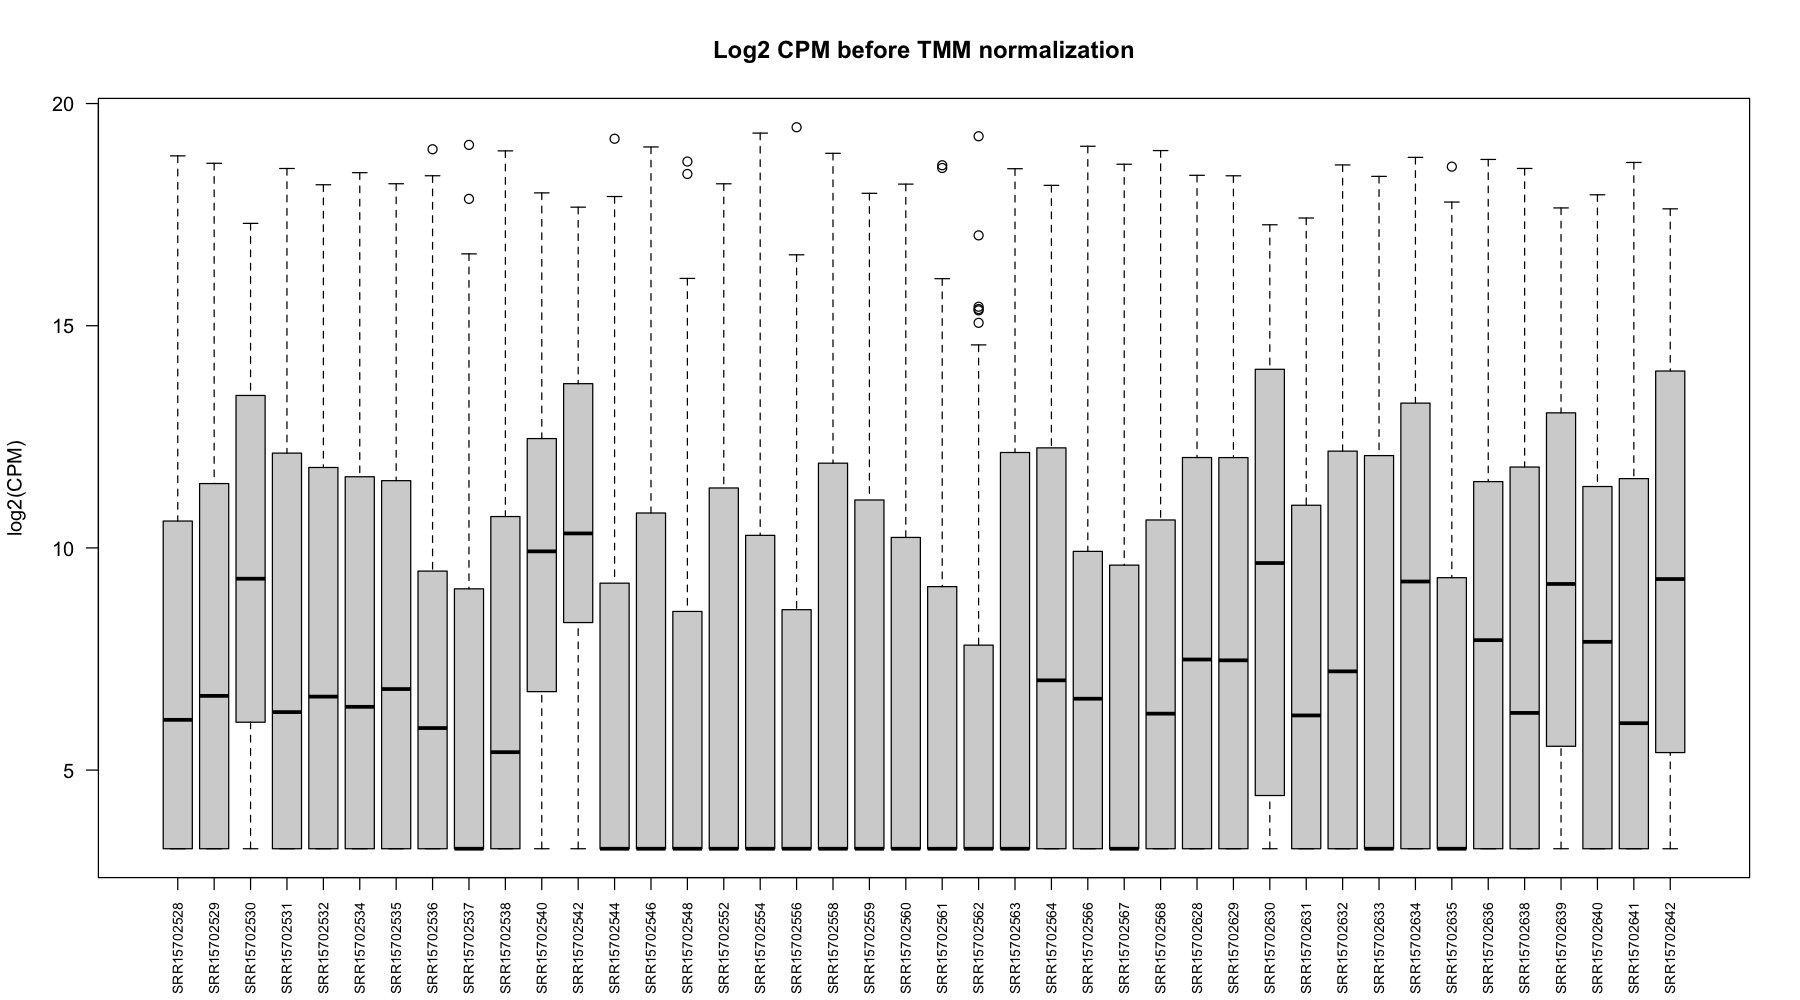
\includegraphics[width=1\linewidth,height=\textheight,keepaspectratio]{../results/plot/differential_abudance/log2_CPM_before_TMM.png}

}

\caption{\label{fig-tmm-before}Log2 counts-per-million before TMM
normalization.}

\end{figure}%

\begin{figure}[H]

\centering{

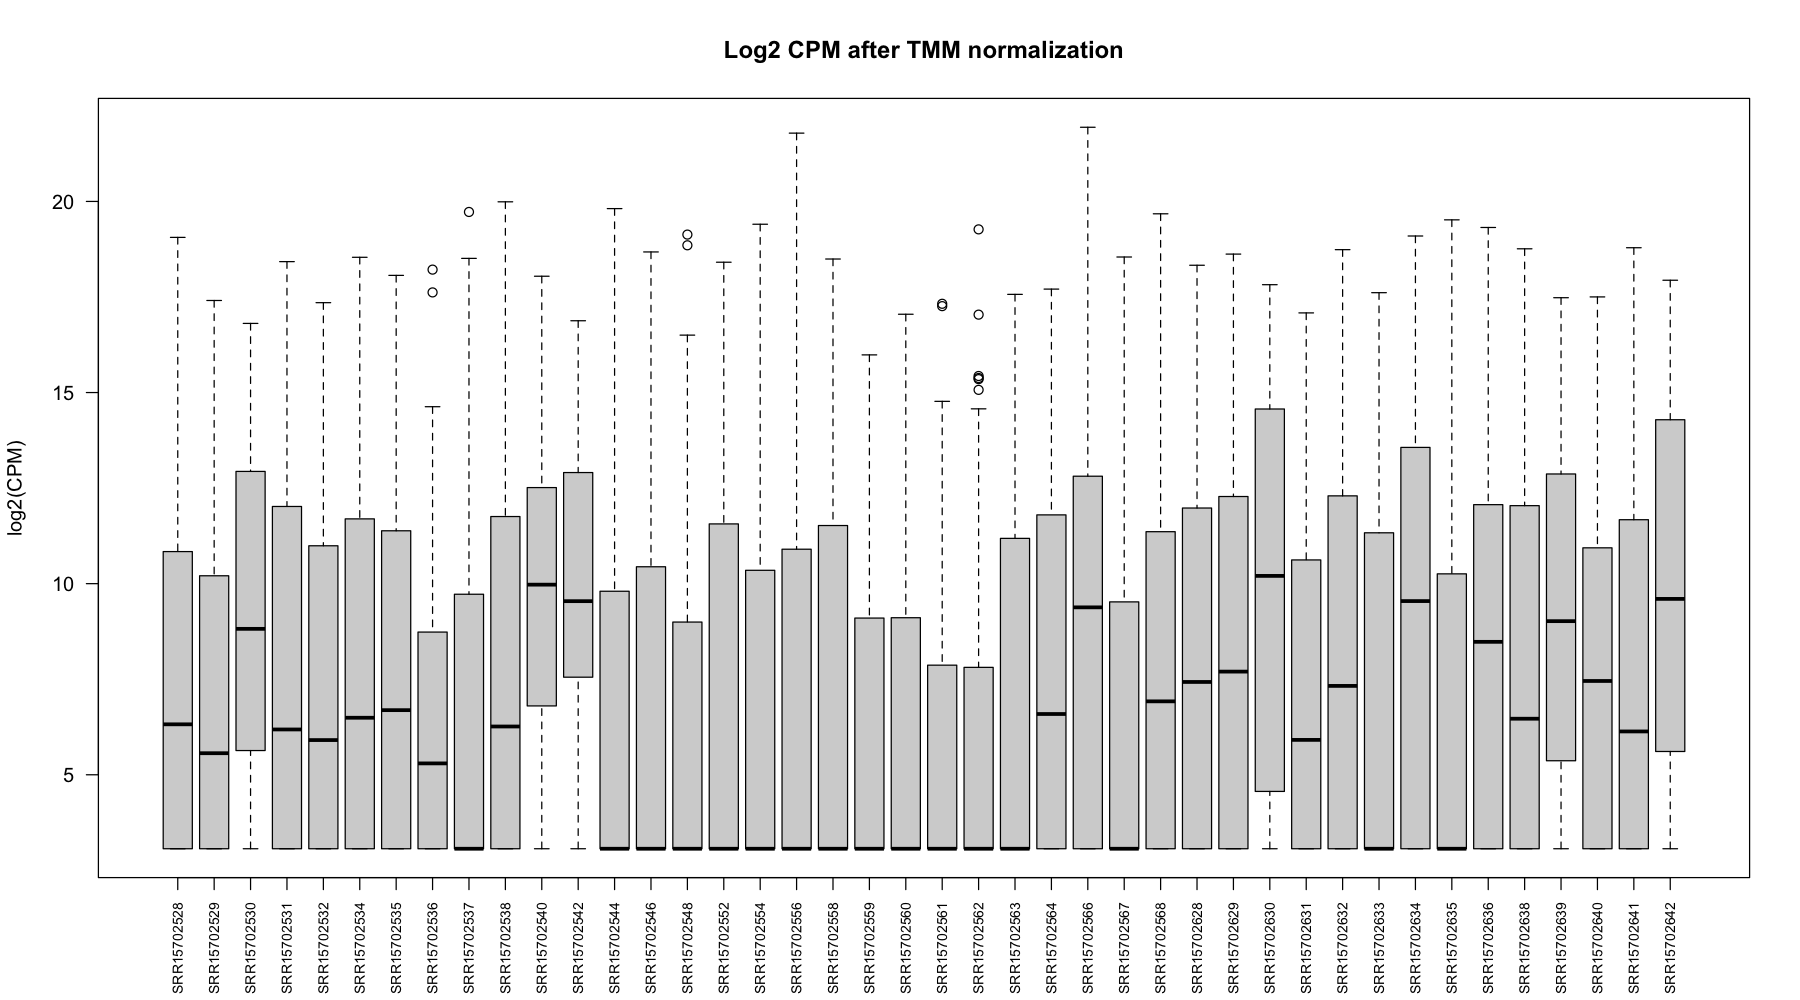
\includegraphics[width=1\linewidth,height=\textheight,keepaspectratio]{../results/plot/differential_abudance/log2_CPM_after_TMM.png}

}

\caption{\label{fig-tmm-after}Log2 counts-per-million after TMM
normalization.}

\end{figure}%

Exploratory ordinations of the normalized data (MDS and PCA; Appendix)
showed a partial separation between groups.

The exact test identified 28 taxa with BH-FDR \textless{} 0.25: 12
enriched and 16 depleted in UC (Figure~\ref{fig-volcano},
Table~\ref{tbl-da}, Figure~\ref{fig-heatmap}). Sixteen of them also
passed FDR \textless{} 0.05. The strongest signals included enrichment
of Enterobacteriaceae, Morganellaceae, Neisseriaceae, Porphyromonadaceae
and Fusobacteriaceae in UC, together with depletion of
Methanobacteriaceae, Barnesiellaceae and the {[}Eubacterium{]}
coprostanoligenes group.

\begin{figure}[H]

\centering{

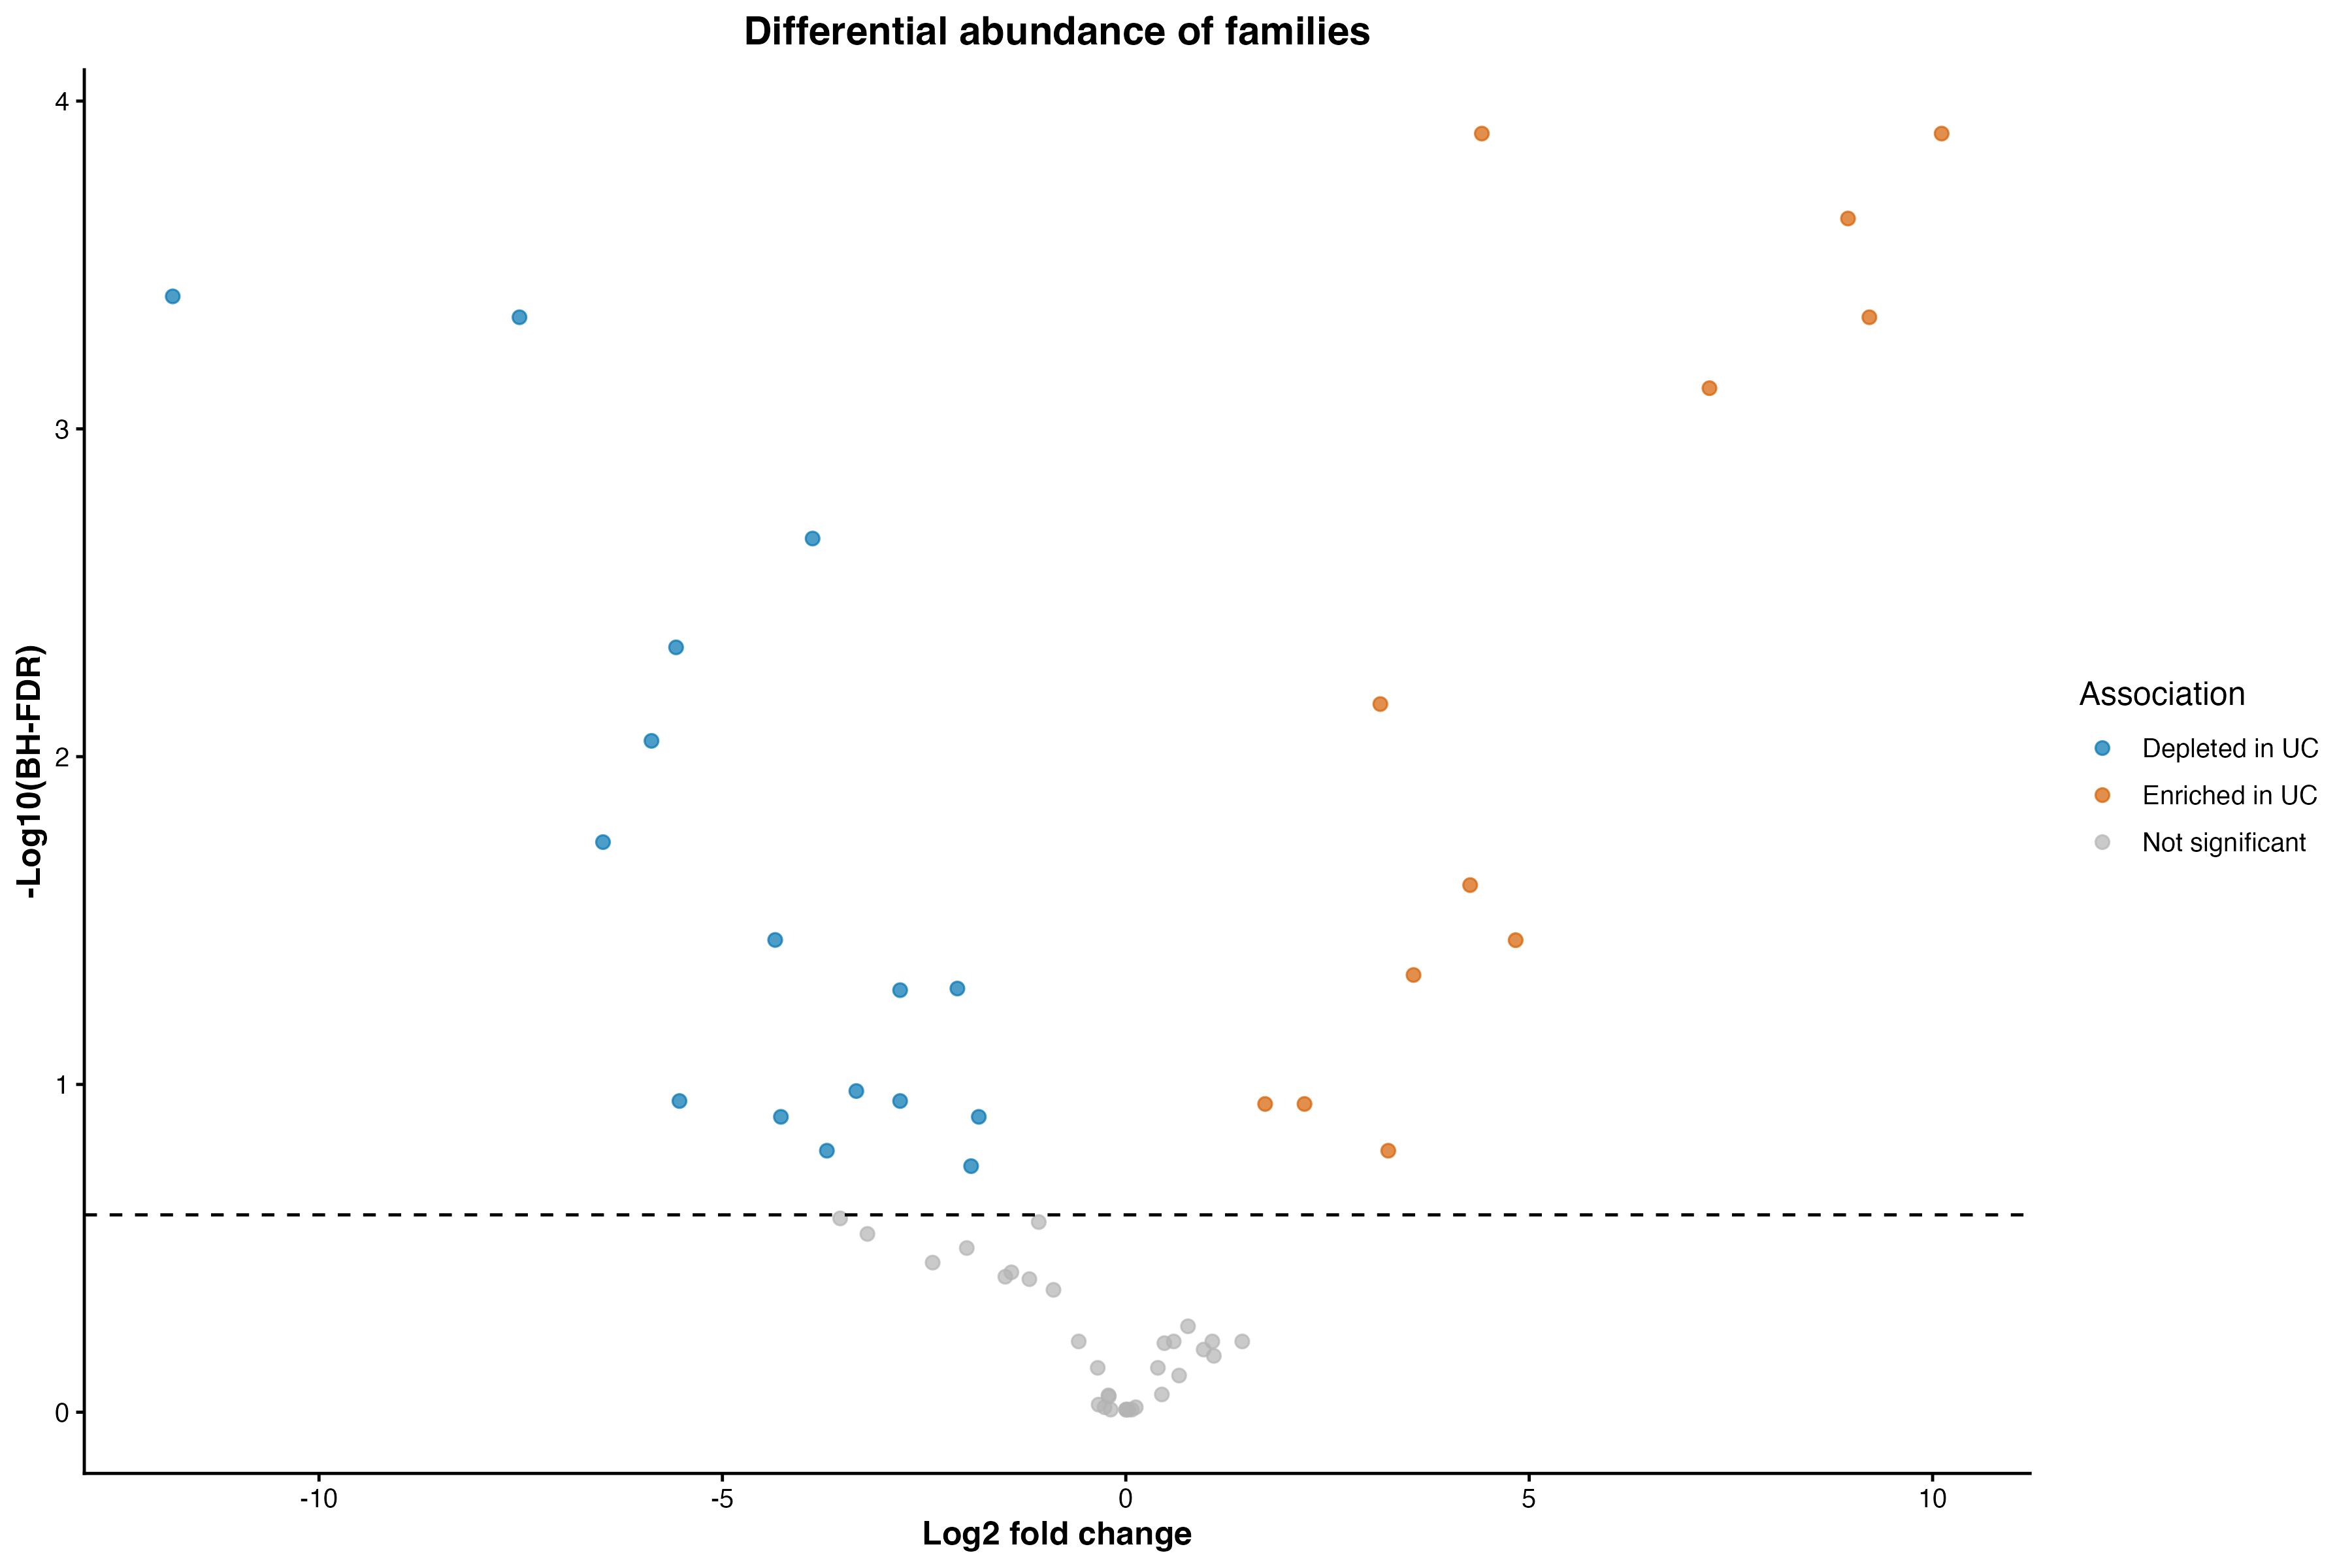
\includegraphics[width=1\linewidth,height=\textheight,keepaspectratio]{../results/plot/differential_abudance/differential_abundance_volcano.png}

}

\caption{\label{fig-volcano}Differential abundance of microbial
families, UC vs Healthy. Points above the dashed line have BH-FDR
\textless{} 0.25.}

\end{figure}%

\begin{longtable}[]{@{}
  >{\raggedright\arraybackslash}p{(\linewidth - 10\tabcolsep) * \real{0.3509}}
  >{\raggedleft\arraybackslash}p{(\linewidth - 10\tabcolsep) * \real{0.2105}}
  >{\raggedleft\arraybackslash}p{(\linewidth - 10\tabcolsep) * \real{0.1491}}
  >{\raggedleft\arraybackslash}p{(\linewidth - 10\tabcolsep) * \real{0.0789}}
  >{\raggedleft\arraybackslash}p{(\linewidth - 10\tabcolsep) * \real{0.0789}}
  >{\raggedright\arraybackslash}p{(\linewidth - 10\tabcolsep) * \real{0.1316}}@{}}

\caption{\label{tbl-da}Taxa differentially abundant between UC and
Healthy (BH-FDR \textless{} 0.25), ordered by FDR. Unclassified lineages
are labelled with their lowest assigned rank.}

\tabularnewline

\toprule\noalign{}
\begin{minipage}[b]{\linewidth}\raggedright
Taxon
\end{minipage} & \begin{minipage}[b]{\linewidth}\raggedleft
log2 FC (UC vs Healthy)
\end{minipage} & \begin{minipage}[b]{\linewidth}\raggedleft
Average log2 CPM
\end{minipage} & \begin{minipage}[b]{\linewidth}\raggedleft
p-value
\end{minipage} & \begin{minipage}[b]{\linewidth}\raggedleft
BH-FDR
\end{minipage} & \begin{minipage}[b]{\linewidth}\raggedright
Direction
\end{minipage} \\
\midrule\noalign{}
\endhead
\bottomrule\noalign{}
\endlastfoot
Enterobacteriaceae & 4.41 & 14.76 & 3.07e-06 & 0.000126 & Enriched in
UC \\
Morganellaceae & 10.11 & 9.05 & 4.26e-06 & 0.000126 & Enriched in UC \\
Neisseriaceae & 8.95 & 9.46 & 1.16e-05 & 0.000228 & Enriched in UC \\
Methanobacteriaceae & -11.81 & 11.02 & 2.67e-05 & 0.000394 & Depleted in
UC \\
Barnesiellaceae & -7.52 & 12.02 & 4.28e-05 & 0.000457 & Depleted in
UC \\
Porphyromonadaceae & 9.22 & 12.17 & 4.64e-05 & 0.000457 & Enriched in
UC \\
Fusobacteriaceae & 7.23 & 12.52 & 8.92e-05 & 0.000751 & Enriched in
UC \\
{[}Eubacterium{]} coprostanoligenes group & -3.88 & 11.98 & 0.000293 &
0.00216 & Depleted in UC \\
Unclassified (order Chloroplast) & -5.57 & 6.48 & 0.000708 & 0.00464 &
Depleted in UC \\
Pasteurellaceae & 3.15 & 13.07 & 0.00117 & 0.00691 & Enriched in UC \\
Moraxellaceae & -5.88 & 5.67 & 0.00167 & 0.00895 & Depleted in UC \\
Victivallaceae & -6.48 & 6.09 & 0.00371 & 0.0182 & Depleted in UC \\
Family XI & 4.27 & 10.18 & 0.00543 & 0.0247 & Enriched in UC \\
Unclassified (order Oscillospirales) & -4.35 & 6.82 & 0.0086 & 0.0362 &
Depleted in UC \\
Unclassified (order Bacteroidales) & 4.83 & 9.41 & 0.00923 & 0.0363 &
Enriched in UC \\
Campylobacteraceae & 3.57 & 6.48 & 0.0126 & 0.0464 & Enriched in UC \\
Eggerthellaceae & -2.09 & 11.80 & 0.0147 & 0.051 & Depleted in UC \\
Monoglobaceae & -2.80 & 11.53 & 0.0157 & 0.0516 & Depleted in UC \\
Akkermansiaceae & -3.34 & 14.07 & 0.0337 & 0.105 & Depleted in UC \\
Pseudomonadaceae & -2.80 & 6.62 & 0.0389 & 0.112 & Depleted in UC \\
Unclassified (order RF39) & -5.53 & 12.29 & 0.04 & 0.112 & Depleted in
UC \\
Bacteroidaceae & 1.73 & 18.56 & 0.0441 & 0.115 & Enriched in UC \\
Sutterellaceae & 2.21 & 14.25 & 0.0447 & 0.115 & Enriched in UC \\
Unclassified (order Clostridia UCG-014) & -4.27 & 13.19 & 0.0515 & 0.126
& Depleted in UC \\
Clostridiaceae & -1.82 & 13.69 & 0.0532 & 0.126 & Depleted in UC \\
UCG-010 & -3.70 & 9.53 & 0.0719 & 0.159 & Depleted in UC \\
Carnobacteriaceae & 3.25 & 8.81 & 0.0729 & 0.159 & Enriched in UC \\
Unclassified (class Clostridia) & -1.92 & 7.93 & 0.0842 & 0.178 &
Depleted in UC \\

\end{longtable}

Of the 28 taxa, 22 are named families and 6 are unclassified lineages
(one enriched, annotated at order Bacteroidales; five depleted,
annotated at order Chloroplast, Oscillospirales, RF39, Clostridia
UCG-014 and class Clostridia), which cannot be interpreted at family
level. Two further points call for caution. The order Chloroplast
comprises plant-derived organelle sequences, likely of dietary origin,
which were not removed before the analysis; and Methanobacteriaceae is
an archaeal family amplified by the same primers, so not all depleted
taxa are bacterial. Moreover, several of the strongest signals reflect
presence/absence patterns visible in the heatmap
(Figure~\ref{fig-heatmap}): Morganellaceae and Neisseriaceae are
detected mainly in a subset of UC samples, and Methanobacteriaceae only
in a subset of healthy samples. Log2 fold changes of this size (up to
about 10) derive from these patterns and should be interpreted with
caution.

\begin{figure}[H]

\centering{

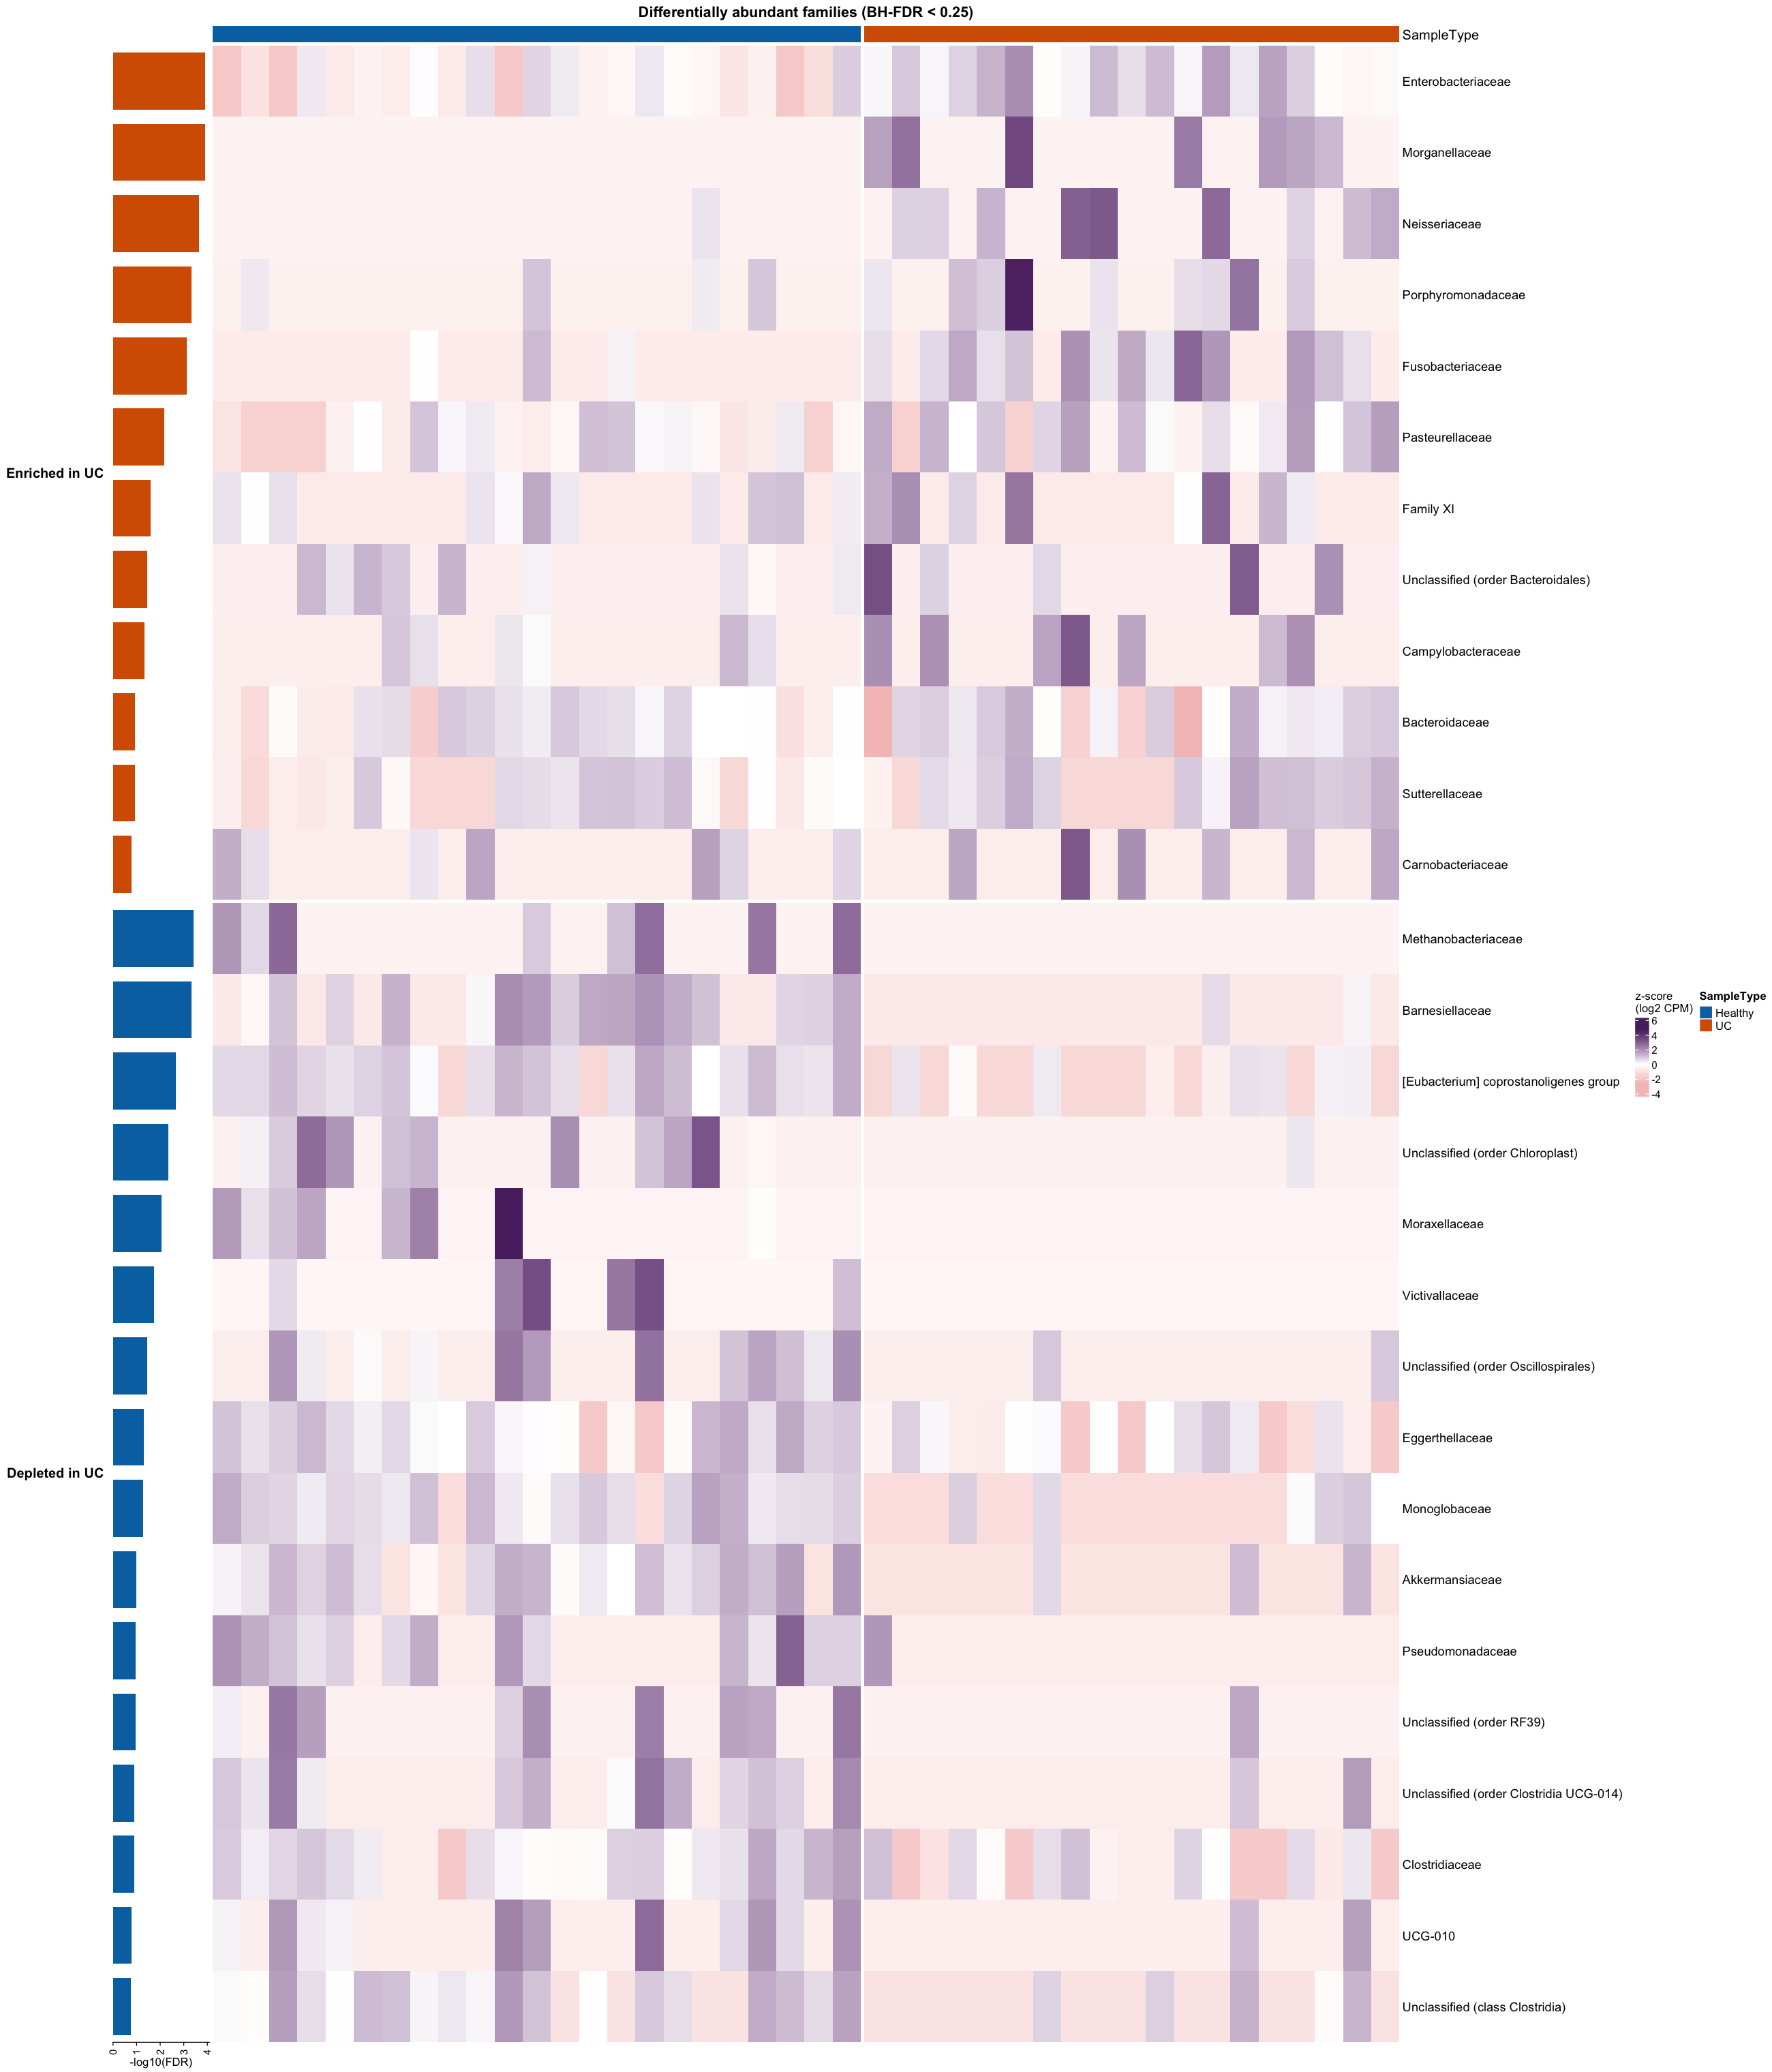
\includegraphics[width=1\linewidth,height=\textheight,keepaspectratio]{../results/plot/differential_abudance/differentially_abundant_families_heatmap.png}

}

\caption{\label{fig-heatmap}Row-scaled log2-CPM (z-score) of the 28
differentially abundant taxa (BH-FDR \textless{} 0.25). Rows are split
by direction of change and ordered by FDR within each block; bars show
-log10(BH-FDR). Unclassified lineages are labelled with their lowest
assigned rank.}

\end{figure}%

\section{Discussion}\label{discussion}

\subsection{Interpretation}\label{interpretation}

The present analysis indicates an alteration of the gut microbiome in
children with UC compared with healthy controls. Alpha diversity was
significantly lower in UC, with a median Shannon index of 2.44 compared
with 2.69 in healthy children (Wilcoxon p = 0.002). This difference
remained evident after adjustment for age and gender, with UC associated
with an approximately 20\% lower Shannon diversity (fold change 0.80,
95\% CI 0.71--0.90, p \textless{} 0.001). At the community-composition
level, disease status explained 9.7\% of the variation in genus-level
Bray--Curtis dissimilarities (PERMANOVA pseudo-F = 4.44, p = 0.001),
whereas age and gender did not reach conventional statistical
significance. Multivariate dispersion did not differ significantly
between groups (F = 0.94, p = 0.329), which suggests that the PERMANOVA
signal mainly reflects differences in community centroids, although the
power of the dispersion test is limited.

The taxonomic profiles were consistent with this broader shift in
community structure. Healthy samples were dominated by Bacillota and
Bacteroidota, whereas UC samples showed a lower relative abundance of
Bacillota and higher Bacteroidota and Pseudomonadota.
Differential-abundance analysis further identified 28 taxa at BH-FDR
\textless{} 0.25 (22 named families and 6 unclassified lineages),
including 12 enriched and 16 depleted in UC, with 16 passing the more
stringent FDR \textless{} 0.05 threshold. Among the strongest signals,
Enterobacteriaceae, Morganellaceae and Neisseriaceae were enriched in
UC, whereas Methanobacteriaceae, Barnesiellaceae and the
{[}Eubacterium{]} coprostanoligenes group were depleted. The expansion
of Enterobacteriaceae-related taxa is consistent with the well-described
association between intestinal inflammation and facultative anaerobic
Proteobacteria (Pseudomonadota), whereas depletion of taxa belonging to
anaerobic and potentially metabolically beneficial groups may reflect
disruption of the healthy intestinal microbial ecosystem. These
taxonomic changes should nevertheless be interpreted as associations
rather than evidence of causality.

Taken together, the alpha-diversity, beta-diversity and
differential-abundance results are consistent with UC-associated
microbiome dysbiosis. The lower Shannon diversity indicates reduced
within-sample community complexity, while PERMANOVA indicates that UC
status is also associated with a shift in overall community composition.
Differential-abundance analysis identifies specific taxonomic features
that accompany this separation, including expansion of
Enterobacteriaceae-related taxa and depletion of several anaerobic taxa.

\subsection{Comparison with the original
study}\label{comparison-with-the-original-study}

Zuo et al.~(2022) reported that pediatric UC was characterized by a
dysbiotic and less diverse gut microbial population, with some species
of the Christensenellaceae family depleted and some species of the
Enterobacteriaceae family enriched, and reported broadly similar
findings between 16S rRNA and shotgun metagenomic data for alpha
diversity, beta diversity and prediction accuracy. In the present
analysis, alpha diversity was concordant with these findings, with
significantly lower Shannon diversity in UC, and community composition
was also concordant, with disease status significantly associated with
genus-level Bray--Curtis community structure. Enterobacteriaceae were
among the differentially abundant families in the present analysis and
were strongly enriched in UC (log2 fold change = 4.41, BH-FDR = 1.26 ×
10⁻⁴). In contrast, Christensenellaceae were not differentially abundant
in the present analysis (P = 0.229, BH-FDR = 0.386), and therefore the
reported Christensenellaceae depletion could not be reproduced at the
family level in this analysis.

Differences between the studies are expected because the present
analysis tested differential abundance at the family level, whereas Zuo
et al.~also resolved taxonomic differences at the species level. In
addition, the analytical frameworks differed, including TMM
normalization and the edgeR exact test used here, as well as differences
in feature filtering and potentially in the reference taxonomy.
Consequently, absence of a significant Christensenellaceae signal in the
present family-level analysis does not necessarily contradict
species-level depletion reported by Zuo et al.; species-specific changes
can be obscured when taxa are aggregated to a higher taxonomic level.

\subsection{Limitations}\label{limitations}

\begin{itemize}
\tightlist
\item
  \textbf{Sample size.} With 42 children, power is limited, in
  particular for the family-level tests, where an FDR threshold of 0.25
  was used. Results should be considered exploratory and in need of
  validation.
\item
  \textbf{Cross-sectional design and confounding.} The data come from a
  single time point. Age and gender were accounted for in alpha and beta
  diversity, but not in the differential abundance test, which compares
  two groups only. Treatment-related variables available in the metadata
  (antibiotics, biologics, steroids, aminosalicylates, immunomodulators)
  were not modelled and may influence the UC microbiome.
\item
  \textbf{Compositionality.} 16S data are relative. Differences in the
  abundance of one family can reflect changes in other families; TMM
  normalization mitigates but does not remove this limitation, and
  results are interpreted as differences in observed relative abundance,
  not absolute abundance.
\item
  \textbf{Sparse signals.} Several differentially abundant taxa are
  detected in only a subset of samples of one group and absent in the
  other; the corresponding fold changes are large but statistically
  fragile.
\item
  \textbf{Non-bacterial and non-microbial sequences.} Plant organelle
  (chloroplast) sequences were not filtered out, and the primers also
  amplify archaea; one significant taxon belongs to each category.
\item
  \textbf{Resolution of the V4 region.} Taxonomic assignment is reliable
  mainly to genus level; species-level calls are exact matches and
  should be interpreted with caution.
\item
  \textbf{Taxonomic aggregation.} ASVs without annotation at the chosen
  rank are retained as separate unclassified units (6 of the 28
  significant taxa), and the unclassified fraction (32.21\% of ASVs at
  genus level) cannot be interpreted biologically.
\item
  \textbf{Distance choice.} Beta diversity was based on Bray-Curtis
  dissimilarities of relative abundances; phylogeny-based metrics
  (UniFrac) and compositional distances (Aitchison) were not used.
\end{itemize}

\subsection{Possible extensions}\label{possible-extensions}

\begin{itemize}
\tightlist
\item
  Removal of chloroplast and mitochondrial sequences, and separate
  handling of archaea, before the diversity and differential-abundance
  analyses.
\item
  Differential abundance with covariate adjustment (age, gender,
  treatment), for example an edgeR generalized linear model or a
  compositional method, as a sensitivity analysis.
\item
  Genus-level differential abundance for a more direct comparison with
  the original study.
\item
  Phylogenetic tree construction and UniFrac distances.
\item
  Integration with the shotgun metagenomic data of the same cohort.
\end{itemize}

\section{Conclusions}\label{conclusions}

\begin{itemize}
\tightlist
\item
  \textbf{Alpha diversity:} UC children showed significantly lower
  genus-level Shannon diversity than healthy children, with the
  difference remaining significant after adjustment for age, gender and
  sequencing depth, and at every rarefaction depth tested.
\item
  \textbf{Community composition:} UC was associated with a distinct
  genus-level community composition, explaining approximately 9.7\% of
  Bray--Curtis variation after accounting for age and gender; dispersion
  did not differ significantly between groups.
\item
  \textbf{Differential abundance:} family-level analysis identified 28
  differentially abundant taxa (22 named families and 6 unclassified
  lineages) at BH-FDR \textless{} 0.25, 12 enriched and 16 depleted in
  UC; 16 also met the more stringent FDR \textless{} 0.05 threshold.
  Enterobacteriaceae-related taxa were among the strongest UC-enriched
  signals, whereas Methanobacteriaceae and Barnesiellaceae were among
  the strongest depleted taxa.
\item
  \textbf{Overall microbiome profile:} taken together, the results
  support a less diverse and compositionally distinct gut microbiome in
  pediatric UC. The findings are exploratory and should be validated in
  larger, independent cohorts with more comprehensive adjustment for
  treatment and other clinical confounders.
\end{itemize}

\section{Reproducibility}\label{reproducibility}

The analysis is fully scripted and organized in six modules
(\texttt{download\_16S\_fastq.sh}, \texttt{qc.sh}, \texttt{01\_dada2.r},
\texttt{02\_phyloseq\_beta\_diversity.r},
\texttt{03\_phyloseq\_alpha\_diversity.r},
\texttt{04\_differential\_abundance\_analysis.r}). The R environment is
managed with \texttt{renv}, random seeds are fixed, and the session
information of each script is saved in the log directory. Instructions
to rerun the analysis are in the repository README.

\section{References}\label{references}

\begin{itemize}
\tightlist
\item
  Zuo W, Wang B, Bai X, et al.~(2022). 16S rRNA and metagenomic shotgun
  sequencing data revealed consistent patterns of gut microbiome
  signature in pediatric ulcerative colitis. \emph{Scientific Reports}.
  DOI: 10.1038/s41598-022-07995-7.
\item
  Callahan BJ, McMurdie PJ, Rosen MJ, et al.~(2016). DADA2:
  High-resolution sample inference from Illumina amplicon data.
  \emph{Nature Methods}, 13:581--583.
\item
  Quast C, Pruesse E, Yilmaz P, et al.~(2013). The SILVA ribosomal RNA
  gene database project. \emph{Nucleic Acids Research}, 41:D590--D596.
\item
  McMurdie PJ, Holmes S. (2013). phyloseq: An R package for reproducible
  interactive analysis and graphics of microbiome census data.
  \emph{PLoS ONE}, 8:e61217.
\item
  McMurdie PJ, Holmes S. (2014). Waste not, want not: why rarefying
  microbiome data is inadmissible. \emph{PLoS Computational Biology},
  10:e1003531.
\item
  Anderson MJ. (2001). A new method for non-parametric multivariate
  analysis of variance. \emph{Austral Ecology}, 26:32--46.
\item
  Lichstein JW. (2007). Multiple regression on distance matrices: a
  multivariate spatial analysis tool. \emph{Plant Ecology},
  188:117--131.
\item
  Robinson MD, McCarthy DJ, Smyth GK. (2010). edgeR: a Bioconductor
  package for differential expression analysis of digital gene
  expression data. \emph{Bioinformatics}, 26:139--140.
\item
  Robinson MD, Oshlack A. (2010). A scaling normalization method for
  differential expression analysis of RNA-seq data. \emph{Genome
  Biology}, 11:R25.
\item
  Gloor GB, Macklaim JM, Pawlowsky-Glahn V, Egozcue JJ. (2017).
  Microbiome datasets are compositional: and this is not optional.
  \emph{Frontiers in Microbiology}, 8:2224.
\end{itemize}

\section{Appendix}\label{appendix}

\subsection{Supplementary figures}\label{supplementary-figures}

\begin{figure}[H]

\centering{

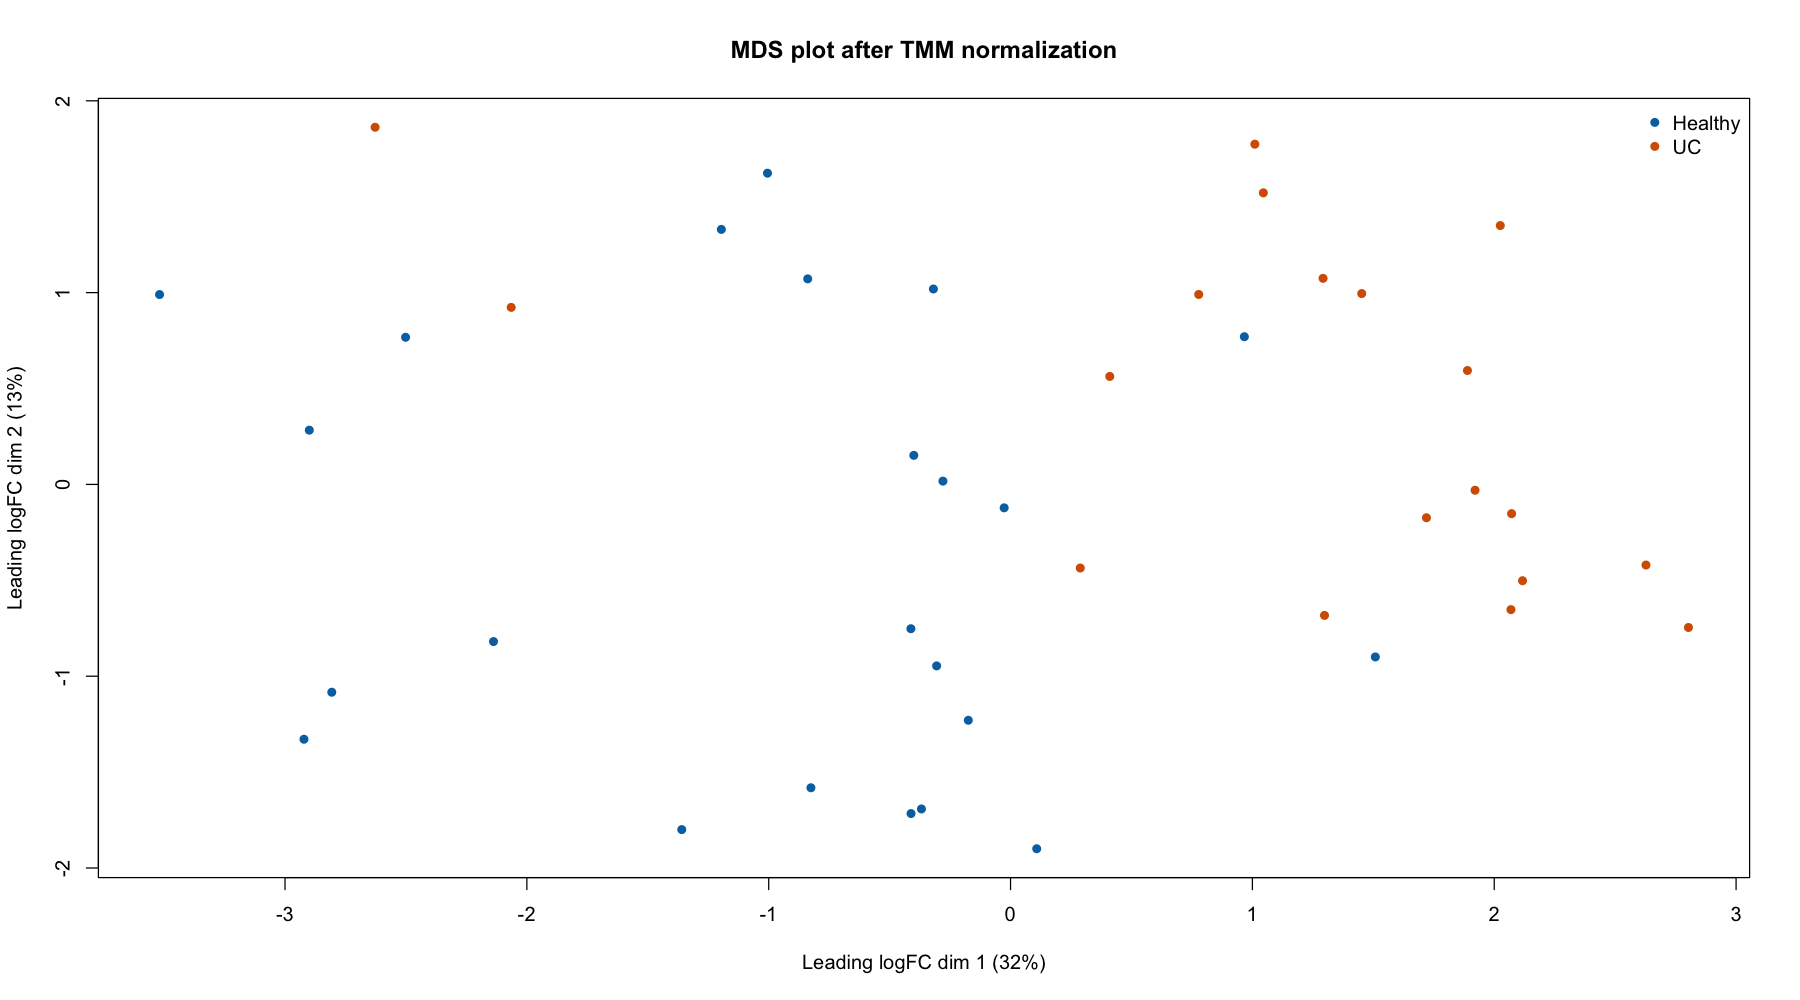
\includegraphics[width=1\linewidth,height=\textheight,keepaspectratio]{../results/plot/differential_abudance/MDS_plot_TMM.png}

}

\caption{\label{fig-mds}MDS of the TMM-normalized family-level data.}

\end{figure}%

\begin{figure}[H]

\centering{

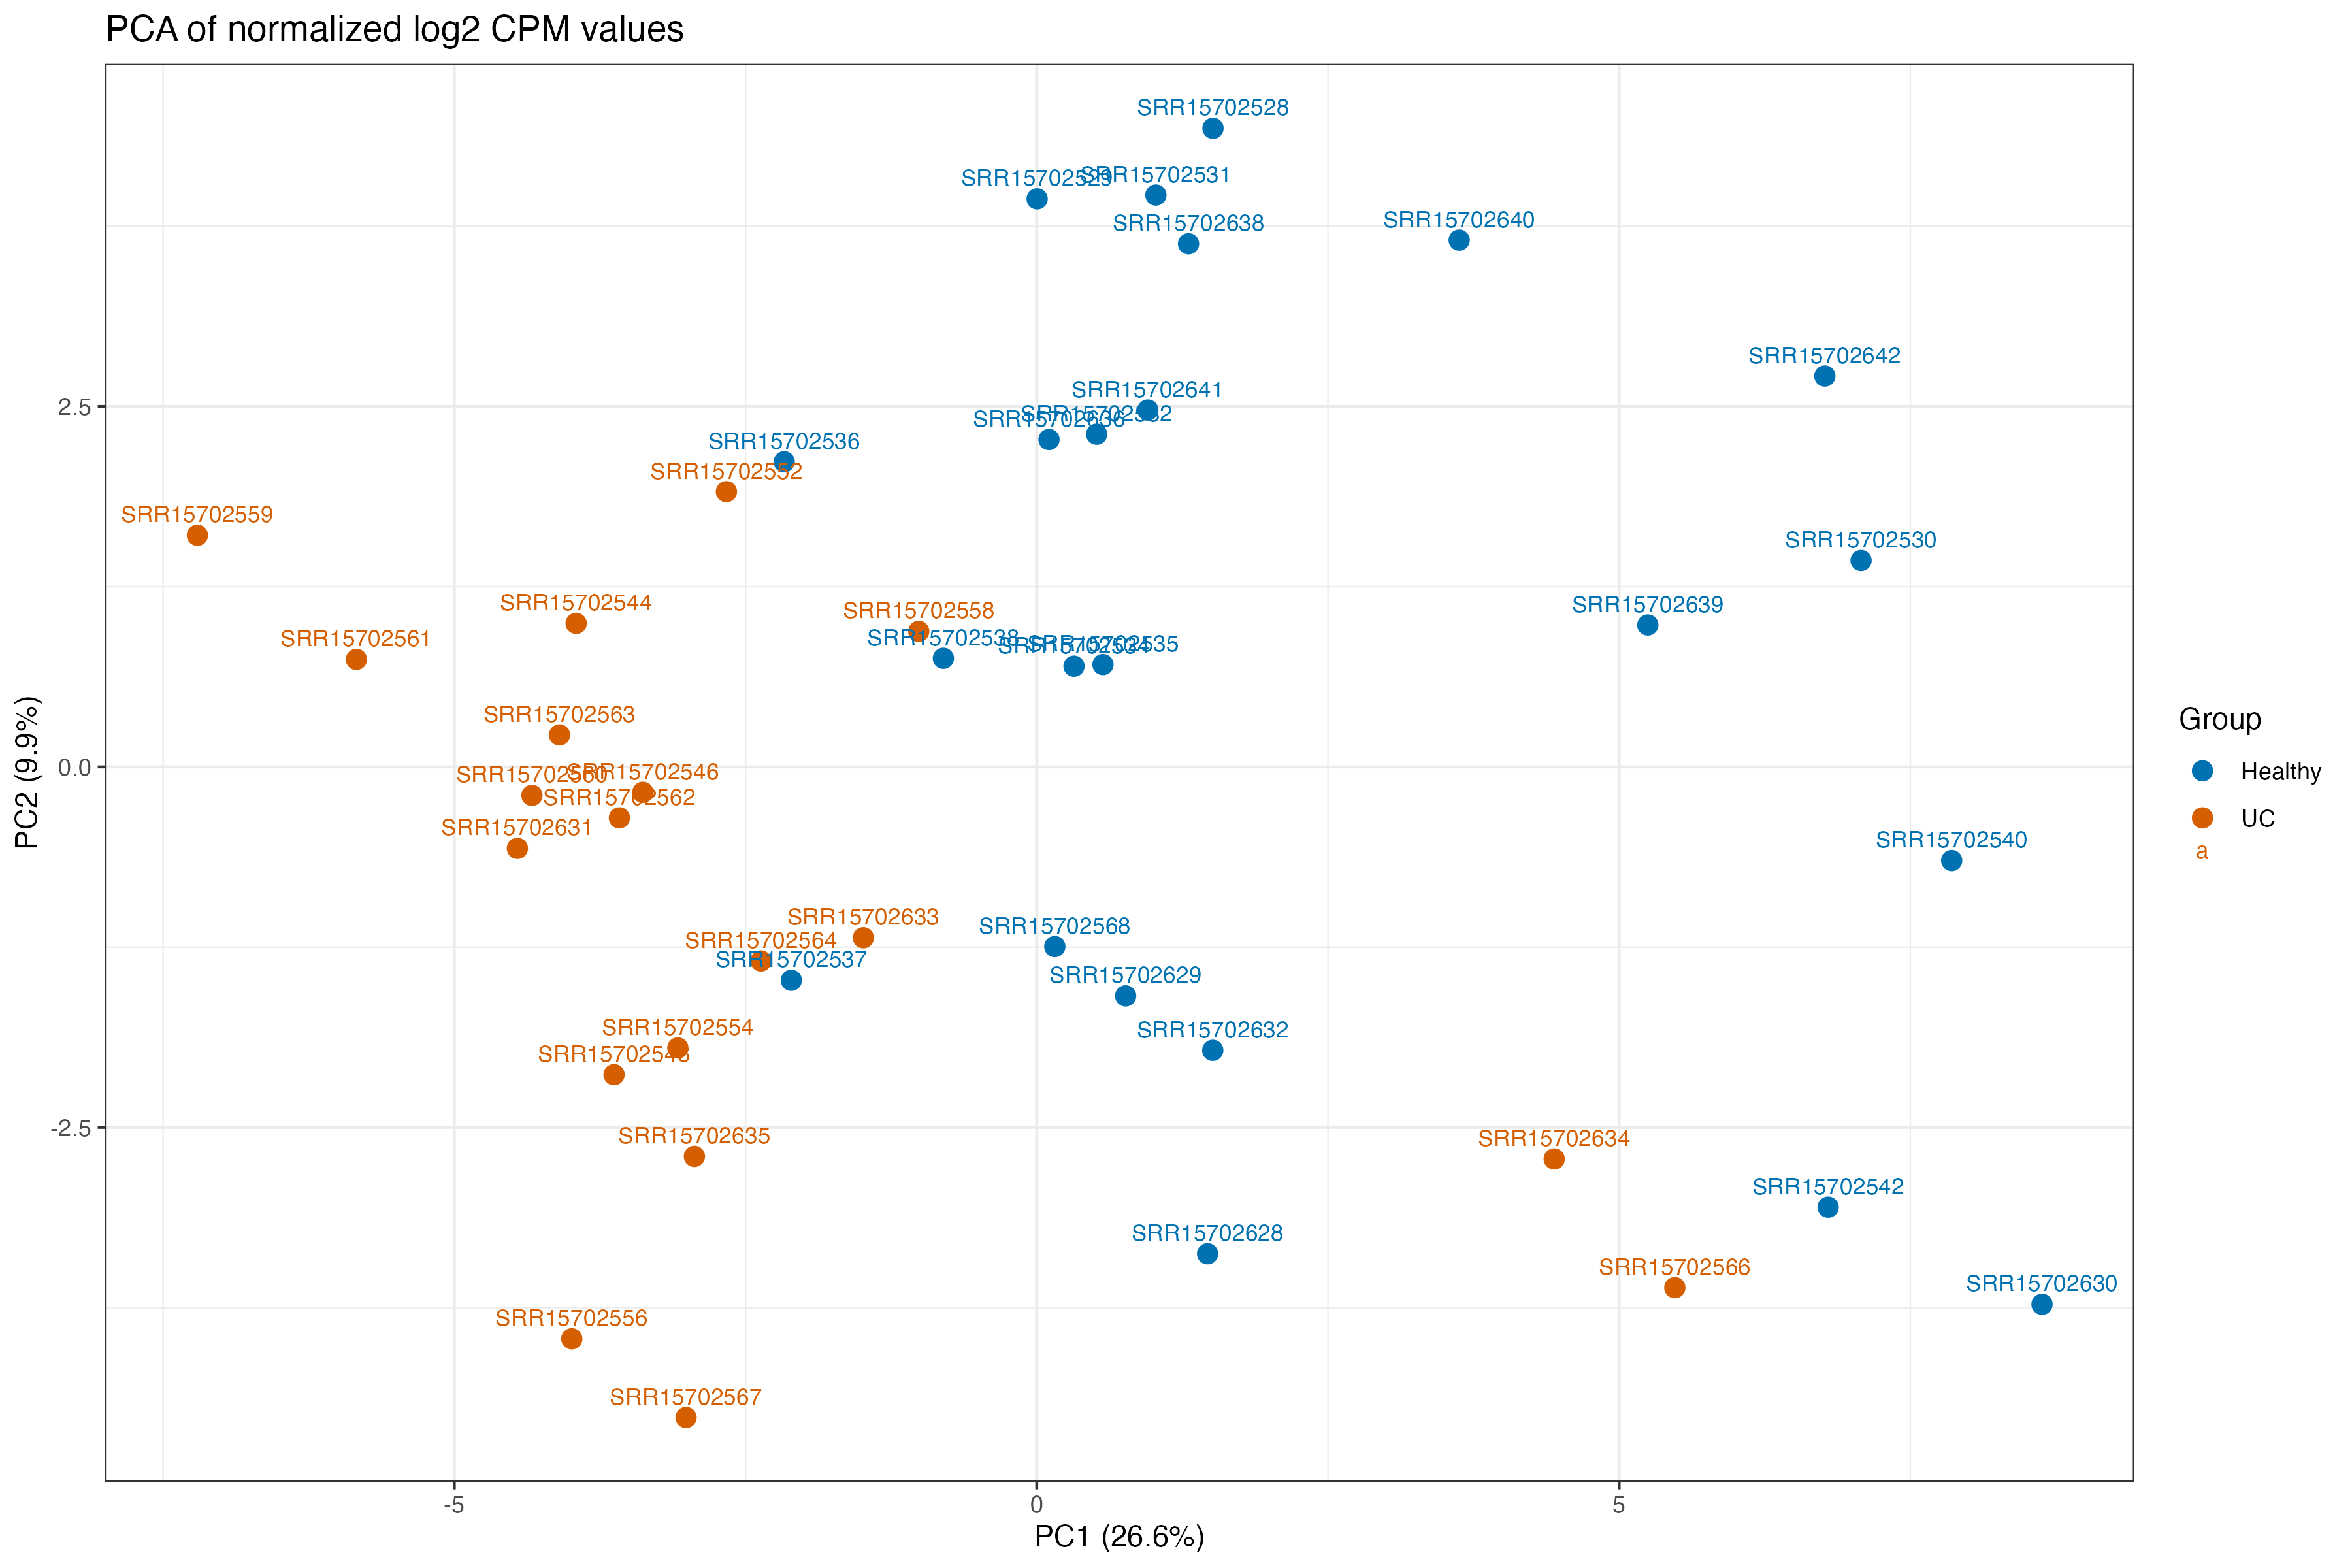
\includegraphics[width=1\linewidth,height=\textheight,keepaspectratio]{../results/plot/differential_abudance/PCA_normalized_log2CPM.png}

}

\caption{\label{fig-pca}PCA of the normalized log2-CPM values.}

\end{figure}%

\begin{figure}[H]

\centering{

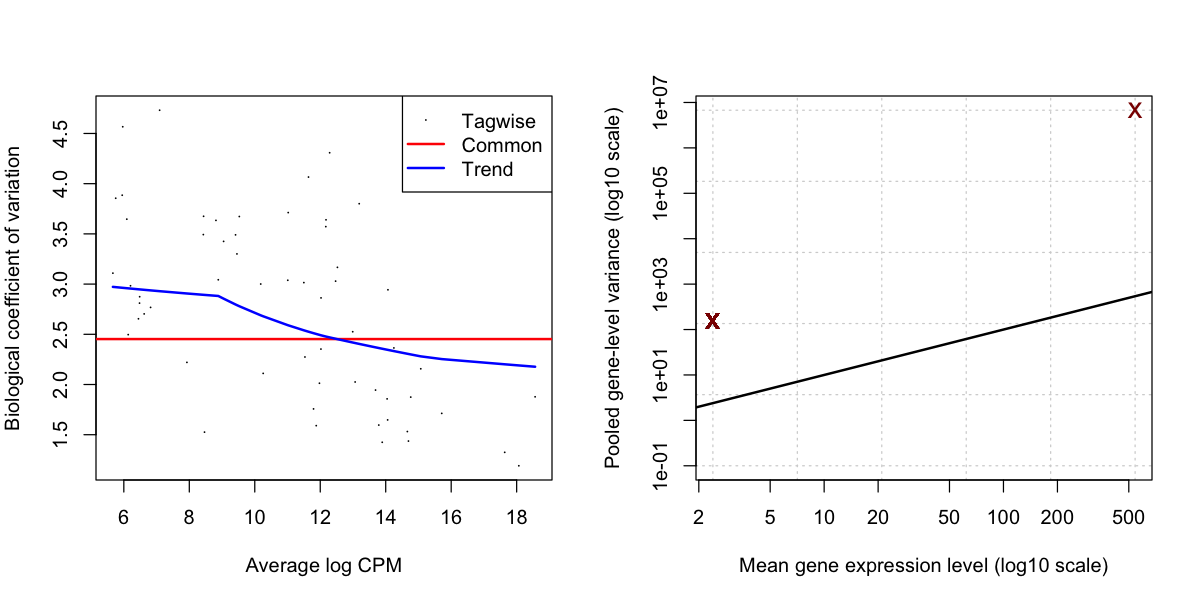
\includegraphics[width=1\linewidth,height=\textheight,keepaspectratio]{../results/plot/differential_abudance/BCV_and_meanVariance_plots.png}

}

\caption{\label{fig-bcv}Biological coefficient of variation (left) and
mean-variance relationship (right) from the edgeR dispersion estimates.}

\end{figure}%

\begin{figure}[H]

\centering{

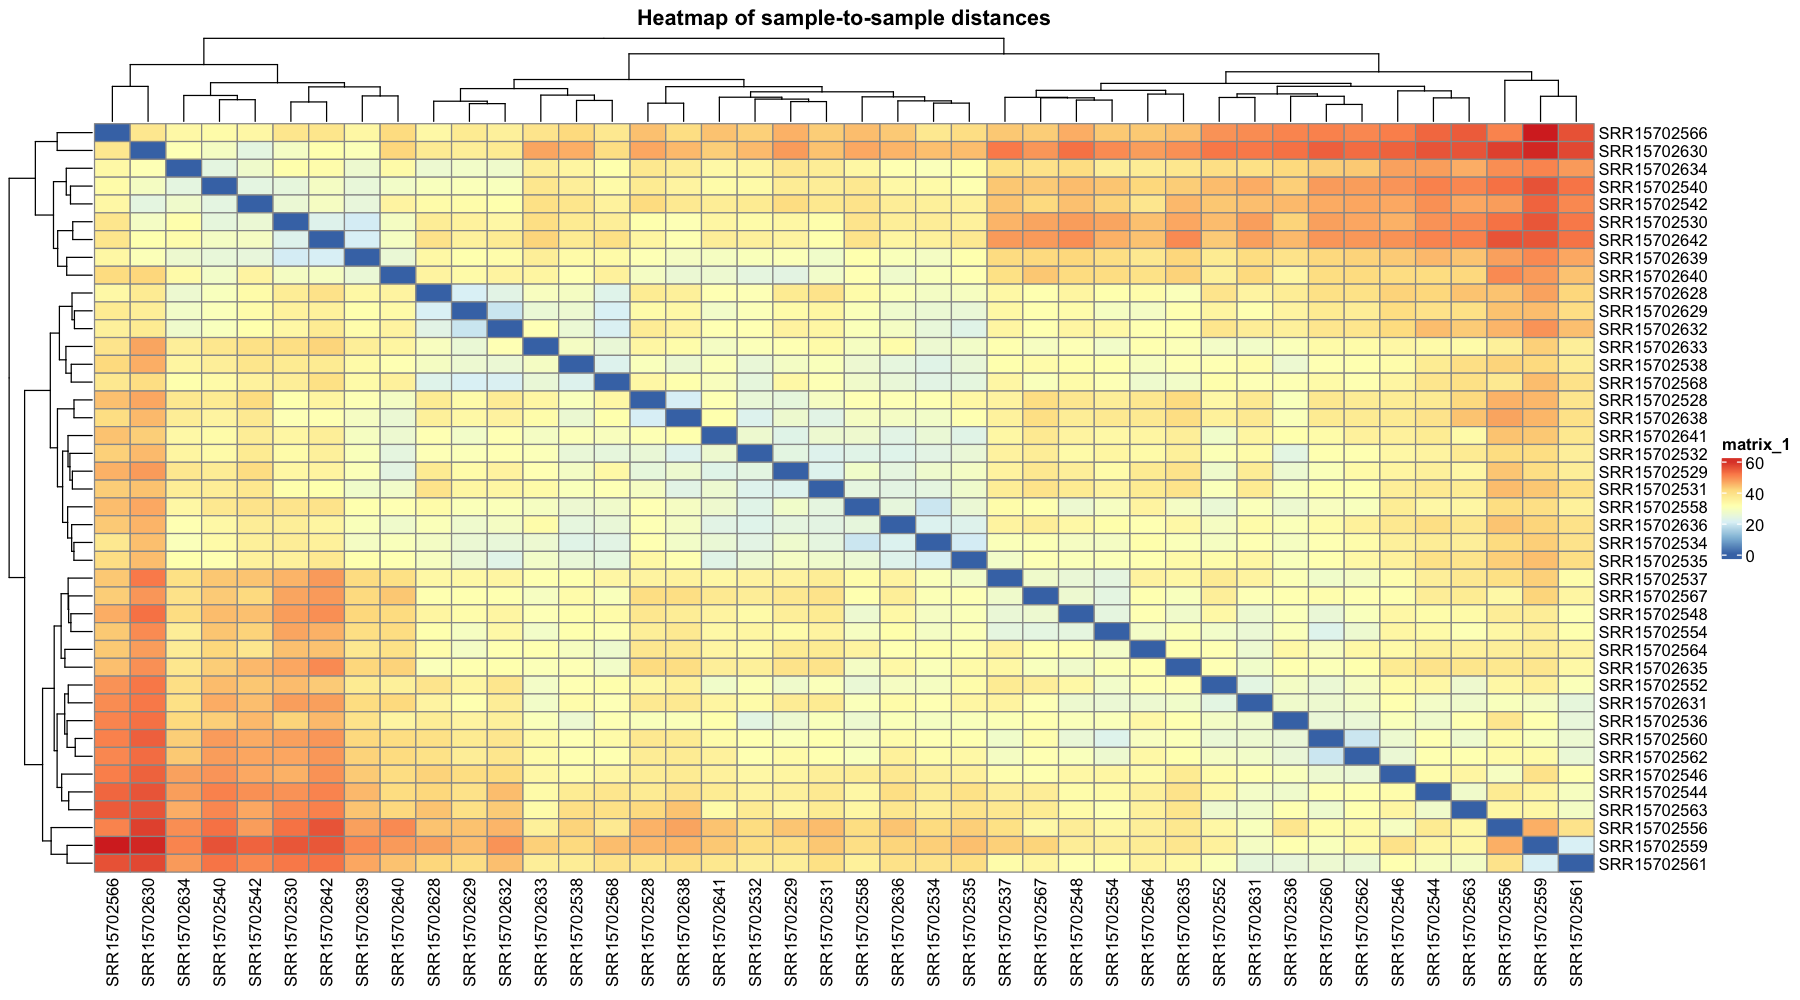
\includegraphics[width=1\linewidth,height=\textheight,keepaspectratio]{../results/plot/differential_abudance/sample_distance_heatmap.png}

}

\caption{\label{fig-sampledist}Sample-to-sample Euclidean distances on
normalized log2-CPM.}

\end{figure}%

\begin{figure}[H]

\centering{

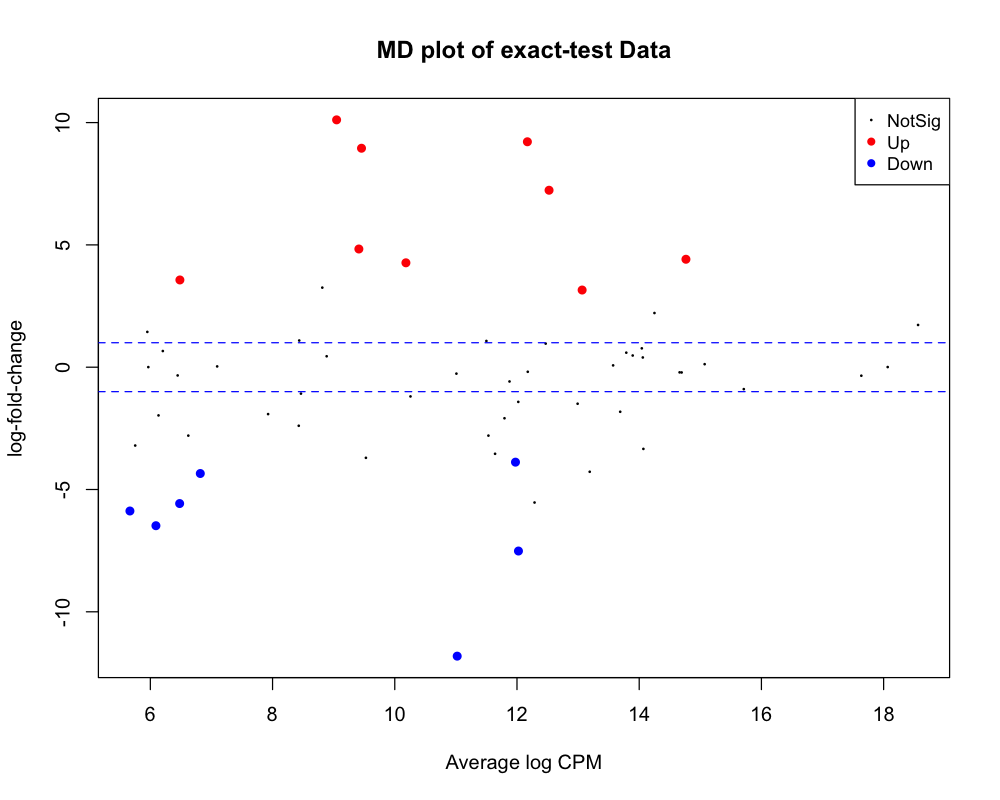
\includegraphics[width=1\linewidth,height=\textheight,keepaspectratio]{../results/plot/differential_abudance/MD_plot_exactTest.png}

}

\caption{\label{fig-md}Mean-difference (MD) plot of the exact test.}

\end{figure}%

\subsection{Main analysis parameters}\label{main-analysis-parameters}

\begin{longtable}[]{@{}
  >{\raggedright\arraybackslash}p{(\linewidth - 4\tabcolsep) * \real{0.2778}}
  >{\raggedright\arraybackslash}p{(\linewidth - 4\tabcolsep) * \real{0.3889}}
  >{\raggedright\arraybackslash}p{(\linewidth - 4\tabcolsep) * \real{0.3333}}@{}}
\caption{Main parameters used in the analysis.}\tabularnewline
\toprule\noalign{}
\begin{minipage}[b]{\linewidth}\raggedright
Step
\end{minipage} & \begin{minipage}[b]{\linewidth}\raggedright
Parameter
\end{minipage} & \begin{minipage}[b]{\linewidth}\raggedright
Value
\end{minipage} \\
\midrule\noalign{}
\endfirsthead
\toprule\noalign{}
\begin{minipage}[b]{\linewidth}\raggedright
Step
\end{minipage} & \begin{minipage}[b]{\linewidth}\raggedright
Parameter
\end{minipage} & \begin{minipage}[b]{\linewidth}\raggedright
Value
\end{minipage} \\
\midrule\noalign{}
\endhead
\bottomrule\noalign{}
\endlastfoot
Filtering & Truncation lengths (F/R) & 140 / 130 bp \\
Filtering & Maximum expected errors (F/R) & 2 / 2 \\
Filtering & Ambiguous bases & 0 \\
Chimera removal & Method & consensus \\
Taxonomy & Reference & SILVA 138.2 (nr99 training set + species file) \\
Alpha diversity & Index / level & Shannon / genus \\
Rarefaction & Depths, repetitions & 1K, 5K, 10K, 30K, 50K, 100K; 100 \\
Beta diversity & Distance / level & Bray-Curtis / genus \\
PERMANOVA, betadisper, MRM & Permutations, seed & 999, 1234 \\
Differential abundance & Level / normalization / test & family / TMM /
exact test \\
Differential abundance & Filters & zero counts \textless{} 90\% of
samples; variance ≥ 0.5 × median \\
Differential abundance & Significance & BH-FDR \textless{} 0.25 \\
\end{longtable}

\subsection{Software environment}\label{software-environment}

R v4.6.0. The exact versions of all R packages are recorded in
\texttt{renv.lock}, and the session information of each analysis script
is saved in the log directory of the repository.




\end{document}
